\documentclass[twoside]{book}

% Packages required by doxygen
\usepackage{fixltx2e}
\usepackage{calc}
\usepackage{doxygen}
\usepackage[export]{adjustbox} % also loads graphicx
\usepackage{graphicx}
\usepackage[utf8]{inputenc}
\usepackage{makeidx}
\usepackage{multicol}
\usepackage{multirow}
\PassOptionsToPackage{warn}{textcomp}
\usepackage{textcomp}
\usepackage[nointegrals]{wasysym}
\usepackage[table]{xcolor}

% Font selection
\usepackage[T1]{fontenc}
\usepackage[scaled=.90]{helvet}
\usepackage{courier}
\usepackage{amssymb}
\usepackage{sectsty}
\renewcommand{\familydefault}{\sfdefault}
\allsectionsfont{%
  \fontseries{bc}\selectfont%
  \color{darkgray}%
}
\renewcommand{\DoxyLabelFont}{%
  \fontseries{bc}\selectfont%
  \color{darkgray}%
}
\newcommand{\+}{\discretionary{\mbox{\scriptsize$\hookleftarrow$}}{}{}}

% Page & text layout
\usepackage{geometry}
\geometry{%
  a4paper,%
  top=2.5cm,%
  bottom=2.5cm,%
  left=2.5cm,%
  right=2.5cm%
}
\tolerance=750
\hfuzz=15pt
\hbadness=750
\setlength{\emergencystretch}{15pt}
\setlength{\parindent}{0cm}
\setlength{\parskip}{3ex plus 2ex minus 2ex}
\makeatletter
\renewcommand{\paragraph}{%
  \@startsection{paragraph}{4}{0ex}{-1.0ex}{1.0ex}{%
    \normalfont\normalsize\bfseries\SS@parafont%
  }%
}
\renewcommand{\subparagraph}{%
  \@startsection{subparagraph}{5}{0ex}{-1.0ex}{1.0ex}{%
    \normalfont\normalsize\bfseries\SS@subparafont%
  }%
}
\makeatother

% Headers & footers
\usepackage{fancyhdr}
\pagestyle{fancyplain}
\fancyhead[LE]{\fancyplain{}{\bfseries\thepage}}
\fancyhead[CE]{\fancyplain{}{}}
\fancyhead[RE]{\fancyplain{}{\bfseries\leftmark}}
\fancyhead[LO]{\fancyplain{}{\bfseries\rightmark}}
\fancyhead[CO]{\fancyplain{}{}}
\fancyhead[RO]{\fancyplain{}{\bfseries\thepage}}
\fancyfoot[LE]{\fancyplain{}{}}
\fancyfoot[CE]{\fancyplain{}{}}
\fancyfoot[RE]{\fancyplain{}{\bfseries\scriptsize Generated by Doxygen }}
\fancyfoot[LO]{\fancyplain{}{\bfseries\scriptsize Generated by Doxygen }}
\fancyfoot[CO]{\fancyplain{}{}}
\fancyfoot[RO]{\fancyplain{}{}}
\renewcommand{\footrulewidth}{0.4pt}
\renewcommand{\chaptermark}[1]{%
  \markboth{#1}{}%
}
\renewcommand{\sectionmark}[1]{%
  \markright{\thesection\ #1}%
}

% Indices & bibliography
\usepackage{natbib}
\usepackage[titles]{tocloft}
\setcounter{tocdepth}{3}
\setcounter{secnumdepth}{5}
\makeindex

% Hyperlinks (required, but should be loaded last)
\usepackage{ifpdf}
\ifpdf
  \usepackage[pdftex,pagebackref=true]{hyperref}
\else
  \usepackage[ps2pdf,pagebackref=true]{hyperref}
\fi
\hypersetup{%
  colorlinks=true,%
  linkcolor=blue,%
  citecolor=blue,%
  unicode%
}

% Custom commands
\newcommand{\clearemptydoublepage}{%
  \newpage{\pagestyle{empty}\cleardoublepage}%
}

\usepackage{caption}
\captionsetup{labelsep=space,justification=centering,font={bf},singlelinecheck=off,skip=4pt,position=top}

%===== C O N T E N T S =====

\begin{document}

% Titlepage & ToC
\hypersetup{pageanchor=false,
             bookmarksnumbered=true,
             pdfencoding=unicode
            }
\pagenumbering{alph}
\begin{titlepage}
\vspace*{7cm}
\begin{center}%
{\Large Drum Machine \\[1ex]\large 1.\+0 }\\
\vspace*{1cm}
{\large Generated by Doxygen 1.8.13}\\
\end{center}
\end{titlepage}
\clearemptydoublepage
\pagenumbering{roman}
\tableofcontents
\clearemptydoublepage
\pagenumbering{arabic}
\hypersetup{pageanchor=true}

%--- Begin generated contents ---
\chapter{Namespace Index}
\section{Namespace List}
Here is a list of all namespaces with brief descriptions\+:\begin{DoxyCompactList}
\item\contentsline{section}{\hyperlink{namespacebeat}{beat} }{\pageref{namespacebeat}}{}
\item\contentsline{section}{\hyperlink{namespaceinputs}{inputs} }{\pageref{namespaceinputs}}{}
\item\contentsline{section}{\hyperlink{namespaceoutputs}{outputs} }{\pageref{namespaceoutputs}}{}
\item\contentsline{section}{\hyperlink{namespacesample}{sample} }{\pageref{namespacesample}}{}
\item\contentsline{section}{\hyperlink{namespacestate}{state} }{\pageref{namespacestate}}{}
\end{DoxyCompactList}

\chapter{Hierarchical Index}
\section{Klassenhierarchie}
Die Liste der Ableitungen ist -\/mit Einschränkungen-\/ alphabetisch sortiert\+:\begin{DoxyCompactList}
\item \contentsline{section}{A\+Output\+Controller}{\pageref{class_a_output_controller}}{}
\begin{DoxyCompactList}
\item \contentsline{section}{Rasp\+Output\+Controller}{\pageref{class_rasp_output_controller}}{}
\end{DoxyCompactList}
\item \contentsline{section}{Display}{\pageref{class_display}}{}
\item \contentsline{section}{Drum\+Machine}{\pageref{class_drum_machine}}{}
\item \contentsline{section}{Input\+Listener}{\pageref{class_input_listener}}{}
\begin{DoxyCompactList}
\item \contentsline{section}{Drum\+Machine\+Input\+Listener}{\pageref{class_drum_machine_input_listener}}{}
\end{DoxyCompactList}
\item \contentsline{section}{Rasp\+Input\+Controller}{\pageref{class_rasp_input_controller}}{}
\item \contentsline{section}{Sample}{\pageref{class_sample}}{}
\item \contentsline{section}{Timer}{\pageref{class_timer}}{}
\end{DoxyCompactList}

\chapter{Class Index}
\section{Auflistung der Klassen}
Hier folgt die Aufzählung aller Klassen, Strukturen, Varianten und Schnittstellen mit einer Kurzbeschreibung\+:\begin{DoxyCompactList}
\item\contentsline{section}{\hyperlink{class_a_output_controller}{A\+Output\+Controller} }{\pageref{class_a_output_controller}}{}
\item\contentsline{section}{\hyperlink{class_display}{Display} }{\pageref{class_display}}{}
\item\contentsline{section}{\hyperlink{class_drum_machine}{Drum\+Machine} }{\pageref{class_drum_machine}}{}
\item\contentsline{section}{\hyperlink{class_drum_machine_input_listener}{Drum\+Machine\+Input\+Listener} }{\pageref{class_drum_machine_input_listener}}{}
\item\contentsline{section}{\hyperlink{class_input_listener}{Input\+Listener} }{\pageref{class_input_listener}}{}
\item\contentsline{section}{\hyperlink{class_rasp_input_controller}{Rasp\+Input\+Controller} }{\pageref{class_rasp_input_controller}}{}
\item\contentsline{section}{\hyperlink{class_rasp_output_controller}{Rasp\+Output\+Controller} }{\pageref{class_rasp_output_controller}}{}
\item\contentsline{section}{\hyperlink{class_sample}{Sample} \\*A class that holds and maintains information about a sample audio file, which can be played by the Drum Machine }{\pageref{class_sample}}{}
\item\contentsline{section}{\hyperlink{class_timer}{Timer} }{\pageref{class_timer}}{}
\end{DoxyCompactList}

\chapter{File Index}
\section{File List}
Here is a list of all files with brief descriptions\+:\begin{DoxyCompactList}
\item\contentsline{section}{\hyperlink{_a_output_controller_8h}{A\+Output\+Controller.\+h} }{\pageref{_a_output_controller_8h}}{}
\item\contentsline{section}{\hyperlink{_display_8cpp}{Display.\+cpp} }{\pageref{_display_8cpp}}{}
\item\contentsline{section}{\hyperlink{_display_8h}{Display.\+h} }{\pageref{_display_8h}}{}
\item\contentsline{section}{\hyperlink{_drum_machine_8cpp}{Drum\+Machine.\+cpp} }{\pageref{_drum_machine_8cpp}}{}
\item\contentsline{section}{\hyperlink{_drum_machine_8h}{Drum\+Machine.\+h} }{\pageref{_drum_machine_8h}}{}
\item\contentsline{section}{\hyperlink{_drum_machine_input_listener_8cpp}{Drum\+Machine\+Input\+Listener.\+cpp} }{\pageref{_drum_machine_input_listener_8cpp}}{}
\item\contentsline{section}{\hyperlink{_drum_machine_input_listener_8h}{Drum\+Machine\+Input\+Listener.\+h} }{\pageref{_drum_machine_input_listener_8h}}{}
\item\contentsline{section}{\hyperlink{_input_listener_8h}{Input\+Listener.\+h} }{\pageref{_input_listener_8h}}{}
\item\contentsline{section}{\hyperlink{main_8cpp}{main.\+cpp} }{\pageref{main_8cpp}}{}
\item\contentsline{section}{\hyperlink{_rasp_input_controller_8cpp}{Rasp\+Input\+Controller.\+cpp} }{\pageref{_rasp_input_controller_8cpp}}{}
\item\contentsline{section}{\hyperlink{_rasp_input_controller_8h}{Rasp\+Input\+Controller.\+h} }{\pageref{_rasp_input_controller_8h}}{}
\item\contentsline{section}{\hyperlink{_rasp_output_controller_8cpp}{Rasp\+Output\+Controller.\+cpp} }{\pageref{_rasp_output_controller_8cpp}}{}
\item\contentsline{section}{\hyperlink{_rasp_output_controller_8h}{Rasp\+Output\+Controller.\+h} }{\pageref{_rasp_output_controller_8h}}{}
\item\contentsline{section}{\hyperlink{_sample_8cpp}{Sample.\+cpp} }{\pageref{_sample_8cpp}}{}
\item\contentsline{section}{\hyperlink{_sample_8h}{Sample.\+h} }{\pageref{_sample_8h}}{}
\item\contentsline{section}{\hyperlink{_timer_8cpp}{Timer.\+cpp} }{\pageref{_timer_8cpp}}{}
\item\contentsline{section}{\hyperlink{_timer_8h}{Timer.\+h} }{\pageref{_timer_8h}}{}
\end{DoxyCompactList}

\chapter{Namespace Documentation}
\hypertarget{namespacebeat}{}\section{beat Namespace Reference}
\label{namespacebeat}\index{beat@{beat}}
\subsection*{Variables}
\begin{DoxyCompactItemize}
\item 
const unsigned short \hyperlink{namespacebeat_ae859561033de8f2140542a8bea7d5f02}{B\+E\+A\+T1} = 0
\item 
const unsigned short \hyperlink{namespacebeat_a219eb8f5f0218df3af3f4d4d9214327f}{B\+E\+A\+T2} = 1
\item 
const unsigned short \hyperlink{namespacebeat_a0ccf0d5bdc6dfdae1fd7b1667655a18f}{B\+E\+A\+T3} = 2
\item 
const unsigned short \hyperlink{namespacebeat_acb66407079f4f750c8edf7c1bd8519df}{B\+E\+A\+T4} = 3
\item 
const unsigned short \hyperlink{namespacebeat_a1707525607992183af84b75b13bdcf1c}{B\+E\+A\+T5} = 4
\item 
const unsigned short \hyperlink{namespacebeat_a38be39fd5d7424553131d77620a5fbfc}{B\+E\+A\+T6} = 5
\item 
const unsigned short \hyperlink{namespacebeat_af4ce75f48a22e0f3aacded8385030cad}{B\+E\+A\+T7} = 6
\item 
const unsigned short \hyperlink{namespacebeat_a564212b647573e2f3fce876049227d2c}{B\+E\+A\+T8} = 7
\item 
const unsigned short \hyperlink{namespacebeat_a6558138490436cdf9a77d90ffd07e092}{B\+E\+A\+T9} = 8
\item 
const unsigned short \hyperlink{namespacebeat_abd0eb0f3160a3579b574ffa8bf94282c}{B\+E\+A\+T10} = 9
\item 
const unsigned short \hyperlink{namespacebeat_a4ba76b47d18db4674af1ca28136614e2}{B\+E\+A\+T11} = 10
\item 
const unsigned short \hyperlink{namespacebeat_ae84780c2b37cac562b4f9e7676d7a715}{B\+E\+A\+T12} = 11
\item 
const unsigned short \hyperlink{namespacebeat_a0056cac49aa9cd40c0532068b40322fe}{B\+E\+A\+T13} = 12
\item 
const unsigned short \hyperlink{namespacebeat_aa25c9d3e796af023ea86fc1181ff4732}{B\+E\+A\+T14} = 13
\item 
const unsigned short \hyperlink{namespacebeat_a241a13409659dff75e5368358447fc73}{B\+E\+A\+T15} = 14
\item 
const unsigned short \hyperlink{namespacebeat_ad619f02c1a78c30570d7371411f1ef47}{B\+E\+A\+T16} = 15
\end{DoxyCompactItemize}


\subsection{Variable Documentation}
\mbox{\Hypertarget{namespacebeat_ae859561033de8f2140542a8bea7d5f02}\label{namespacebeat_ae859561033de8f2140542a8bea7d5f02}} 
\index{beat@{beat}!B\+E\+A\+T1@{B\+E\+A\+T1}}
\index{B\+E\+A\+T1@{B\+E\+A\+T1}!beat@{beat}}
\subsubsection{\texorpdfstring{B\+E\+A\+T1}{BEAT1}}
{\footnotesize\ttfamily const unsigned short beat\+::\+B\+E\+A\+T1 = 0}



Definition at line 21 of file Drum\+Machine.\+h.



Referenced by Drum\+Machine\+Input\+Listener\+::input\+Event().

\mbox{\Hypertarget{namespacebeat_abd0eb0f3160a3579b574ffa8bf94282c}\label{namespacebeat_abd0eb0f3160a3579b574ffa8bf94282c}} 
\index{beat@{beat}!B\+E\+A\+T10@{B\+E\+A\+T10}}
\index{B\+E\+A\+T10@{B\+E\+A\+T10}!beat@{beat}}
\subsubsection{\texorpdfstring{B\+E\+A\+T10}{BEAT10}}
{\footnotesize\ttfamily const unsigned short beat\+::\+B\+E\+A\+T10 = 9}



Definition at line 22 of file Drum\+Machine.\+h.



Referenced by Drum\+Machine\+Input\+Listener\+::input\+Event().

\mbox{\Hypertarget{namespacebeat_a4ba76b47d18db4674af1ca28136614e2}\label{namespacebeat_a4ba76b47d18db4674af1ca28136614e2}} 
\index{beat@{beat}!B\+E\+A\+T11@{B\+E\+A\+T11}}
\index{B\+E\+A\+T11@{B\+E\+A\+T11}!beat@{beat}}
\subsubsection{\texorpdfstring{B\+E\+A\+T11}{BEAT11}}
{\footnotesize\ttfamily const unsigned short beat\+::\+B\+E\+A\+T11 = 10}



Definition at line 22 of file Drum\+Machine.\+h.



Referenced by Drum\+Machine\+Input\+Listener\+::input\+Event().

\mbox{\Hypertarget{namespacebeat_ae84780c2b37cac562b4f9e7676d7a715}\label{namespacebeat_ae84780c2b37cac562b4f9e7676d7a715}} 
\index{beat@{beat}!B\+E\+A\+T12@{B\+E\+A\+T12}}
\index{B\+E\+A\+T12@{B\+E\+A\+T12}!beat@{beat}}
\subsubsection{\texorpdfstring{B\+E\+A\+T12}{BEAT12}}
{\footnotesize\ttfamily const unsigned short beat\+::\+B\+E\+A\+T12 = 11}



Definition at line 22 of file Drum\+Machine.\+h.



Referenced by Drum\+Machine\+Input\+Listener\+::input\+Event().

\mbox{\Hypertarget{namespacebeat_a0056cac49aa9cd40c0532068b40322fe}\label{namespacebeat_a0056cac49aa9cd40c0532068b40322fe}} 
\index{beat@{beat}!B\+E\+A\+T13@{B\+E\+A\+T13}}
\index{B\+E\+A\+T13@{B\+E\+A\+T13}!beat@{beat}}
\subsubsection{\texorpdfstring{B\+E\+A\+T13}{BEAT13}}
{\footnotesize\ttfamily const unsigned short beat\+::\+B\+E\+A\+T13 = 12}



Definition at line 22 of file Drum\+Machine.\+h.



Referenced by Drum\+Machine\+Input\+Listener\+::input\+Event().

\mbox{\Hypertarget{namespacebeat_aa25c9d3e796af023ea86fc1181ff4732}\label{namespacebeat_aa25c9d3e796af023ea86fc1181ff4732}} 
\index{beat@{beat}!B\+E\+A\+T14@{B\+E\+A\+T14}}
\index{B\+E\+A\+T14@{B\+E\+A\+T14}!beat@{beat}}
\subsubsection{\texorpdfstring{B\+E\+A\+T14}{BEAT14}}
{\footnotesize\ttfamily const unsigned short beat\+::\+B\+E\+A\+T14 = 13}



Definition at line 22 of file Drum\+Machine.\+h.



Referenced by Drum\+Machine\+Input\+Listener\+::input\+Event().

\mbox{\Hypertarget{namespacebeat_a241a13409659dff75e5368358447fc73}\label{namespacebeat_a241a13409659dff75e5368358447fc73}} 
\index{beat@{beat}!B\+E\+A\+T15@{B\+E\+A\+T15}}
\index{B\+E\+A\+T15@{B\+E\+A\+T15}!beat@{beat}}
\subsubsection{\texorpdfstring{B\+E\+A\+T15}{BEAT15}}
{\footnotesize\ttfamily const unsigned short beat\+::\+B\+E\+A\+T15 = 14}



Definition at line 22 of file Drum\+Machine.\+h.



Referenced by Drum\+Machine\+Input\+Listener\+::input\+Event().

\mbox{\Hypertarget{namespacebeat_ad619f02c1a78c30570d7371411f1ef47}\label{namespacebeat_ad619f02c1a78c30570d7371411f1ef47}} 
\index{beat@{beat}!B\+E\+A\+T16@{B\+E\+A\+T16}}
\index{B\+E\+A\+T16@{B\+E\+A\+T16}!beat@{beat}}
\subsubsection{\texorpdfstring{B\+E\+A\+T16}{BEAT16}}
{\footnotesize\ttfamily const unsigned short beat\+::\+B\+E\+A\+T16 = 15}



Definition at line 22 of file Drum\+Machine.\+h.



Referenced by Drum\+Machine\+Input\+Listener\+::input\+Event().

\mbox{\Hypertarget{namespacebeat_a219eb8f5f0218df3af3f4d4d9214327f}\label{namespacebeat_a219eb8f5f0218df3af3f4d4d9214327f}} 
\index{beat@{beat}!B\+E\+A\+T2@{B\+E\+A\+T2}}
\index{B\+E\+A\+T2@{B\+E\+A\+T2}!beat@{beat}}
\subsubsection{\texorpdfstring{B\+E\+A\+T2}{BEAT2}}
{\footnotesize\ttfamily const unsigned short beat\+::\+B\+E\+A\+T2 = 1}



Definition at line 21 of file Drum\+Machine.\+h.



Referenced by Drum\+Machine\+Input\+Listener\+::input\+Event().

\mbox{\Hypertarget{namespacebeat_a0ccf0d5bdc6dfdae1fd7b1667655a18f}\label{namespacebeat_a0ccf0d5bdc6dfdae1fd7b1667655a18f}} 
\index{beat@{beat}!B\+E\+A\+T3@{B\+E\+A\+T3}}
\index{B\+E\+A\+T3@{B\+E\+A\+T3}!beat@{beat}}
\subsubsection{\texorpdfstring{B\+E\+A\+T3}{BEAT3}}
{\footnotesize\ttfamily const unsigned short beat\+::\+B\+E\+A\+T3 = 2}



Definition at line 21 of file Drum\+Machine.\+h.



Referenced by Drum\+Machine\+Input\+Listener\+::input\+Event().

\mbox{\Hypertarget{namespacebeat_acb66407079f4f750c8edf7c1bd8519df}\label{namespacebeat_acb66407079f4f750c8edf7c1bd8519df}} 
\index{beat@{beat}!B\+E\+A\+T4@{B\+E\+A\+T4}}
\index{B\+E\+A\+T4@{B\+E\+A\+T4}!beat@{beat}}
\subsubsection{\texorpdfstring{B\+E\+A\+T4}{BEAT4}}
{\footnotesize\ttfamily const unsigned short beat\+::\+B\+E\+A\+T4 = 3}



Definition at line 21 of file Drum\+Machine.\+h.



Referenced by Drum\+Machine\+Input\+Listener\+::input\+Event().

\mbox{\Hypertarget{namespacebeat_a1707525607992183af84b75b13bdcf1c}\label{namespacebeat_a1707525607992183af84b75b13bdcf1c}} 
\index{beat@{beat}!B\+E\+A\+T5@{B\+E\+A\+T5}}
\index{B\+E\+A\+T5@{B\+E\+A\+T5}!beat@{beat}}
\subsubsection{\texorpdfstring{B\+E\+A\+T5}{BEAT5}}
{\footnotesize\ttfamily const unsigned short beat\+::\+B\+E\+A\+T5 = 4}



Definition at line 21 of file Drum\+Machine.\+h.



Referenced by Drum\+Machine\+Input\+Listener\+::input\+Event().

\mbox{\Hypertarget{namespacebeat_a38be39fd5d7424553131d77620a5fbfc}\label{namespacebeat_a38be39fd5d7424553131d77620a5fbfc}} 
\index{beat@{beat}!B\+E\+A\+T6@{B\+E\+A\+T6}}
\index{B\+E\+A\+T6@{B\+E\+A\+T6}!beat@{beat}}
\subsubsection{\texorpdfstring{B\+E\+A\+T6}{BEAT6}}
{\footnotesize\ttfamily const unsigned short beat\+::\+B\+E\+A\+T6 = 5}



Definition at line 21 of file Drum\+Machine.\+h.



Referenced by Drum\+Machine\+Input\+Listener\+::input\+Event().

\mbox{\Hypertarget{namespacebeat_af4ce75f48a22e0f3aacded8385030cad}\label{namespacebeat_af4ce75f48a22e0f3aacded8385030cad}} 
\index{beat@{beat}!B\+E\+A\+T7@{B\+E\+A\+T7}}
\index{B\+E\+A\+T7@{B\+E\+A\+T7}!beat@{beat}}
\subsubsection{\texorpdfstring{B\+E\+A\+T7}{BEAT7}}
{\footnotesize\ttfamily const unsigned short beat\+::\+B\+E\+A\+T7 = 6}



Definition at line 21 of file Drum\+Machine.\+h.



Referenced by Drum\+Machine\+Input\+Listener\+::input\+Event().

\mbox{\Hypertarget{namespacebeat_a564212b647573e2f3fce876049227d2c}\label{namespacebeat_a564212b647573e2f3fce876049227d2c}} 
\index{beat@{beat}!B\+E\+A\+T8@{B\+E\+A\+T8}}
\index{B\+E\+A\+T8@{B\+E\+A\+T8}!beat@{beat}}
\subsubsection{\texorpdfstring{B\+E\+A\+T8}{BEAT8}}
{\footnotesize\ttfamily const unsigned short beat\+::\+B\+E\+A\+T8 = 7}



Definition at line 21 of file Drum\+Machine.\+h.



Referenced by Drum\+Machine\+Input\+Listener\+::input\+Event().

\mbox{\Hypertarget{namespacebeat_a6558138490436cdf9a77d90ffd07e092}\label{namespacebeat_a6558138490436cdf9a77d90ffd07e092}} 
\index{beat@{beat}!B\+E\+A\+T9@{B\+E\+A\+T9}}
\index{B\+E\+A\+T9@{B\+E\+A\+T9}!beat@{beat}}
\subsubsection{\texorpdfstring{B\+E\+A\+T9}{BEAT9}}
{\footnotesize\ttfamily const unsigned short beat\+::\+B\+E\+A\+T9 = 8}



Definition at line 22 of file Drum\+Machine.\+h.



Referenced by Drum\+Machine\+Input\+Listener\+::input\+Event().


\hypertarget{namespaceinputs}{}\section{inputs-\/\+Namensbereichsreferenz}
\label{namespaceinputs}\index{inputs@{inputs}}
\subsection*{Variablen}
\begin{DoxyCompactItemize}
\item 
const unsigned short \hyperlink{namespaceinputs_ab1d58fe937ccabff6ec4011a74028bfb}{V\+O\+L\+U\+M\+E\+\_\+\+B\+P\+M\+\_\+\+U\+P\+\_\+\+B\+U\+T\+T\+ON} = 1
\item 
const unsigned short \hyperlink{namespaceinputs_af3cad6ab00b2670e1710698945d28c17}{V\+O\+L\+U\+M\+E\+\_\+\+B\+P\+M\+\_\+\+D\+O\+W\+N\+\_\+\+B\+U\+T\+T\+ON} = 2
\item 
const unsigned short \hyperlink{namespaceinputs_af0075a72395787966efcec2403306b43}{M\+U\+T\+E\+\_\+\+B\+U\+T\+T\+ON} = 5
\item 
const unsigned short \hyperlink{namespaceinputs_a39dbaf6935309e198c1a0bc6e3468c45}{S\+A\+M\+P\+L\+E1\+\_\+\+B\+U\+T\+T\+ON} = 6
\item 
const unsigned short \hyperlink{namespaceinputs_afcf2086c7f58f801e5654d8e573d928c}{S\+A\+M\+P\+L\+E2\+\_\+\+B\+U\+T\+T\+ON} = 7
\item 
const unsigned short \hyperlink{namespaceinputs_a17158d35ca30fb91c6f9f757ce0d7ccc}{S\+A\+M\+P\+L\+E3\+\_\+\+B\+U\+T\+T\+ON} = 8
\item 
const unsigned short \hyperlink{namespaceinputs_ac9ccac580f0955e454a367ddc6421d78}{S\+A\+M\+P\+L\+E4\+\_\+\+B\+U\+T\+T\+ON} = 9
\item 
const unsigned short \hyperlink{namespaceinputs_ad22ade847b4a38fd418dccda07814551}{S\+A\+M\+P\+L\+E5\+\_\+\+B\+U\+T\+T\+ON} = 10
\item 
const unsigned short \hyperlink{namespaceinputs_a88edcfa8b89df1abcca33bcec05974c4}{S\+A\+M\+P\+L\+E6\+\_\+\+B\+U\+T\+T\+ON} = 11
\item 
const unsigned short \hyperlink{namespaceinputs_a50972dcf524a7b7c420ca75b0ba72a29}{S\+A\+M\+P\+L\+E7\+\_\+\+B\+U\+T\+T\+ON} = 12
\item 
const unsigned short \hyperlink{namespaceinputs_a85f389284c616cd584390d04ad192ced}{S\+A\+M\+P\+L\+E8\+\_\+\+B\+U\+T\+T\+ON} = 13
\item 
const unsigned short \hyperlink{namespaceinputs_af62021422f469c370f42c78a72504a66}{B\+E\+A\+T1\+\_\+\+B\+U\+T\+T\+ON} = 14
\item 
const unsigned short \hyperlink{namespaceinputs_a8cdd33c9e53b617a2cf8bd32a5b74484}{B\+E\+A\+T2\+\_\+\+B\+U\+T\+T\+ON} = 15
\item 
const unsigned short \hyperlink{namespaceinputs_ab60a6fc2188a034f76d3fbe554efe314}{B\+E\+A\+T3\+\_\+\+B\+U\+T\+T\+ON} = 16
\item 
const unsigned short \hyperlink{namespaceinputs_af65f26f63a9572003a2bc49e7955e319}{B\+E\+A\+T4\+\_\+\+B\+U\+T\+T\+ON} = 17
\item 
const unsigned short \hyperlink{namespaceinputs_a8a027829529daa53a24ece7b8334164b}{B\+E\+A\+T5\+\_\+\+B\+U\+T\+T\+ON} = 18
\item 
const unsigned short \hyperlink{namespaceinputs_a6afdc23bce21454342081cf937e47ab9}{B\+E\+A\+T6\+\_\+\+B\+U\+T\+T\+ON} = 19
\item 
const unsigned short \hyperlink{namespaceinputs_ac74e302394a578b31f0cf44df8cbb1a9}{B\+E\+A\+T7\+\_\+\+B\+U\+T\+T\+ON} = 20
\item 
const unsigned short \hyperlink{namespaceinputs_abfcd4d28221c436391131a27402ea620}{B\+E\+A\+T8\+\_\+\+B\+U\+T\+T\+ON} = 21
\item 
const unsigned short \hyperlink{namespaceinputs_af628ea84bf7114a62249d4bb425ed06a}{B\+E\+A\+T9\+\_\+\+B\+U\+T\+T\+ON} = 22
\item 
const unsigned short \hyperlink{namespaceinputs_a9778bcf3a44a9d16ae156bac6d745a24}{B\+E\+A\+T10\+\_\+\+B\+U\+T\+T\+ON} = 23
\item 
const unsigned short \hyperlink{namespaceinputs_ad09e4010a8b08721988599b198645372}{B\+E\+A\+T11\+\_\+\+B\+U\+T\+T\+ON} = 24
\item 
const unsigned short \hyperlink{namespaceinputs_a7b6bb44b9241cac31ff9909c3fc88271}{B\+E\+A\+T12\+\_\+\+B\+U\+T\+T\+ON} = 25
\item 
const unsigned short \hyperlink{namespaceinputs_a8f9d547eaa8c52cebfa64221341f266a}{B\+E\+A\+T13\+\_\+\+B\+U\+T\+T\+ON} = 26
\item 
const unsigned short \hyperlink{namespaceinputs_a4dfd34a5656f72c71f1b2dd8efc963dc}{B\+E\+A\+T14\+\_\+\+B\+U\+T\+T\+ON} = 27
\item 
const unsigned short \hyperlink{namespaceinputs_a1952aa2d27b65c8d8899a1ae1cfb7bb9}{B\+E\+A\+T15\+\_\+\+B\+U\+T\+T\+ON} = 28
\item 
const unsigned short \hyperlink{namespaceinputs_af0f3099a06352ba4eb0808091b908178}{B\+E\+A\+T16\+\_\+\+B\+U\+T\+T\+ON} = 29
\item 
const unsigned short \hyperlink{namespaceinputs_ab1d04ae8b7a7f4d11849c110f20fae10}{S\+T\+A\+R\+T\+\_\+\+S\+T\+O\+P\+\_\+\+B\+U\+T\+T\+ON} = 30
\end{DoxyCompactItemize}


\subsection{Variablen-\/\+Dokumentation}
\mbox{\Hypertarget{namespaceinputs_a9778bcf3a44a9d16ae156bac6d745a24}\label{namespaceinputs_a9778bcf3a44a9d16ae156bac6d745a24}} 
\index{inputs@{inputs}!B\+E\+A\+T10\+\_\+\+B\+U\+T\+T\+ON@{B\+E\+A\+T10\+\_\+\+B\+U\+T\+T\+ON}}
\index{B\+E\+A\+T10\+\_\+\+B\+U\+T\+T\+ON@{B\+E\+A\+T10\+\_\+\+B\+U\+T\+T\+ON}!inputs@{inputs}}
\subsubsection{\texorpdfstring{B\+E\+A\+T10\+\_\+\+B\+U\+T\+T\+ON}{BEAT10\_BUTTON}}
{\footnotesize\ttfamily const unsigned short inputs\+::\+B\+E\+A\+T10\+\_\+\+B\+U\+T\+T\+ON = 23}



Definiert in Zeile 15 der Datei Rasp\+Input\+Controller.\+h.



Wird benutzt von Drum\+Machine\+Input\+Listener\+::input\+Event().

\mbox{\Hypertarget{namespaceinputs_ad09e4010a8b08721988599b198645372}\label{namespaceinputs_ad09e4010a8b08721988599b198645372}} 
\index{inputs@{inputs}!B\+E\+A\+T11\+\_\+\+B\+U\+T\+T\+ON@{B\+E\+A\+T11\+\_\+\+B\+U\+T\+T\+ON}}
\index{B\+E\+A\+T11\+\_\+\+B\+U\+T\+T\+ON@{B\+E\+A\+T11\+\_\+\+B\+U\+T\+T\+ON}!inputs@{inputs}}
\subsubsection{\texorpdfstring{B\+E\+A\+T11\+\_\+\+B\+U\+T\+T\+ON}{BEAT11\_BUTTON}}
{\footnotesize\ttfamily const unsigned short inputs\+::\+B\+E\+A\+T11\+\_\+\+B\+U\+T\+T\+ON = 24}



Definiert in Zeile 15 der Datei Rasp\+Input\+Controller.\+h.



Wird benutzt von Drum\+Machine\+Input\+Listener\+::input\+Event().

\mbox{\Hypertarget{namespaceinputs_a7b6bb44b9241cac31ff9909c3fc88271}\label{namespaceinputs_a7b6bb44b9241cac31ff9909c3fc88271}} 
\index{inputs@{inputs}!B\+E\+A\+T12\+\_\+\+B\+U\+T\+T\+ON@{B\+E\+A\+T12\+\_\+\+B\+U\+T\+T\+ON}}
\index{B\+E\+A\+T12\+\_\+\+B\+U\+T\+T\+ON@{B\+E\+A\+T12\+\_\+\+B\+U\+T\+T\+ON}!inputs@{inputs}}
\subsubsection{\texorpdfstring{B\+E\+A\+T12\+\_\+\+B\+U\+T\+T\+ON}{BEAT12\_BUTTON}}
{\footnotesize\ttfamily const unsigned short inputs\+::\+B\+E\+A\+T12\+\_\+\+B\+U\+T\+T\+ON = 25}



Definiert in Zeile 16 der Datei Rasp\+Input\+Controller.\+h.



Wird benutzt von Drum\+Machine\+Input\+Listener\+::input\+Event().

\mbox{\Hypertarget{namespaceinputs_a8f9d547eaa8c52cebfa64221341f266a}\label{namespaceinputs_a8f9d547eaa8c52cebfa64221341f266a}} 
\index{inputs@{inputs}!B\+E\+A\+T13\+\_\+\+B\+U\+T\+T\+ON@{B\+E\+A\+T13\+\_\+\+B\+U\+T\+T\+ON}}
\index{B\+E\+A\+T13\+\_\+\+B\+U\+T\+T\+ON@{B\+E\+A\+T13\+\_\+\+B\+U\+T\+T\+ON}!inputs@{inputs}}
\subsubsection{\texorpdfstring{B\+E\+A\+T13\+\_\+\+B\+U\+T\+T\+ON}{BEAT13\_BUTTON}}
{\footnotesize\ttfamily const unsigned short inputs\+::\+B\+E\+A\+T13\+\_\+\+B\+U\+T\+T\+ON = 26}



Definiert in Zeile 16 der Datei Rasp\+Input\+Controller.\+h.



Wird benutzt von Drum\+Machine\+Input\+Listener\+::input\+Event().

\mbox{\Hypertarget{namespaceinputs_a4dfd34a5656f72c71f1b2dd8efc963dc}\label{namespaceinputs_a4dfd34a5656f72c71f1b2dd8efc963dc}} 
\index{inputs@{inputs}!B\+E\+A\+T14\+\_\+\+B\+U\+T\+T\+ON@{B\+E\+A\+T14\+\_\+\+B\+U\+T\+T\+ON}}
\index{B\+E\+A\+T14\+\_\+\+B\+U\+T\+T\+ON@{B\+E\+A\+T14\+\_\+\+B\+U\+T\+T\+ON}!inputs@{inputs}}
\subsubsection{\texorpdfstring{B\+E\+A\+T14\+\_\+\+B\+U\+T\+T\+ON}{BEAT14\_BUTTON}}
{\footnotesize\ttfamily const unsigned short inputs\+::\+B\+E\+A\+T14\+\_\+\+B\+U\+T\+T\+ON = 27}



Definiert in Zeile 16 der Datei Rasp\+Input\+Controller.\+h.



Wird benutzt von Drum\+Machine\+Input\+Listener\+::input\+Event().

\mbox{\Hypertarget{namespaceinputs_a1952aa2d27b65c8d8899a1ae1cfb7bb9}\label{namespaceinputs_a1952aa2d27b65c8d8899a1ae1cfb7bb9}} 
\index{inputs@{inputs}!B\+E\+A\+T15\+\_\+\+B\+U\+T\+T\+ON@{B\+E\+A\+T15\+\_\+\+B\+U\+T\+T\+ON}}
\index{B\+E\+A\+T15\+\_\+\+B\+U\+T\+T\+ON@{B\+E\+A\+T15\+\_\+\+B\+U\+T\+T\+ON}!inputs@{inputs}}
\subsubsection{\texorpdfstring{B\+E\+A\+T15\+\_\+\+B\+U\+T\+T\+ON}{BEAT15\_BUTTON}}
{\footnotesize\ttfamily const unsigned short inputs\+::\+B\+E\+A\+T15\+\_\+\+B\+U\+T\+T\+ON = 28}



Definiert in Zeile 16 der Datei Rasp\+Input\+Controller.\+h.



Wird benutzt von Drum\+Machine\+Input\+Listener\+::input\+Event().

\mbox{\Hypertarget{namespaceinputs_af0f3099a06352ba4eb0808091b908178}\label{namespaceinputs_af0f3099a06352ba4eb0808091b908178}} 
\index{inputs@{inputs}!B\+E\+A\+T16\+\_\+\+B\+U\+T\+T\+ON@{B\+E\+A\+T16\+\_\+\+B\+U\+T\+T\+ON}}
\index{B\+E\+A\+T16\+\_\+\+B\+U\+T\+T\+ON@{B\+E\+A\+T16\+\_\+\+B\+U\+T\+T\+ON}!inputs@{inputs}}
\subsubsection{\texorpdfstring{B\+E\+A\+T16\+\_\+\+B\+U\+T\+T\+ON}{BEAT16\_BUTTON}}
{\footnotesize\ttfamily const unsigned short inputs\+::\+B\+E\+A\+T16\+\_\+\+B\+U\+T\+T\+ON = 29}



Definiert in Zeile 17 der Datei Rasp\+Input\+Controller.\+h.



Wird benutzt von Drum\+Machine\+Input\+Listener\+::input\+Event().

\mbox{\Hypertarget{namespaceinputs_af62021422f469c370f42c78a72504a66}\label{namespaceinputs_af62021422f469c370f42c78a72504a66}} 
\index{inputs@{inputs}!B\+E\+A\+T1\+\_\+\+B\+U\+T\+T\+ON@{B\+E\+A\+T1\+\_\+\+B\+U\+T\+T\+ON}}
\index{B\+E\+A\+T1\+\_\+\+B\+U\+T\+T\+ON@{B\+E\+A\+T1\+\_\+\+B\+U\+T\+T\+ON}!inputs@{inputs}}
\subsubsection{\texorpdfstring{B\+E\+A\+T1\+\_\+\+B\+U\+T\+T\+ON}{BEAT1\_BUTTON}}
{\footnotesize\ttfamily const unsigned short inputs\+::\+B\+E\+A\+T1\+\_\+\+B\+U\+T\+T\+ON = 14}



Definiert in Zeile 13 der Datei Rasp\+Input\+Controller.\+h.



Wird benutzt von Drum\+Machine\+Input\+Listener\+::input\+Event().

\mbox{\Hypertarget{namespaceinputs_a8cdd33c9e53b617a2cf8bd32a5b74484}\label{namespaceinputs_a8cdd33c9e53b617a2cf8bd32a5b74484}} 
\index{inputs@{inputs}!B\+E\+A\+T2\+\_\+\+B\+U\+T\+T\+ON@{B\+E\+A\+T2\+\_\+\+B\+U\+T\+T\+ON}}
\index{B\+E\+A\+T2\+\_\+\+B\+U\+T\+T\+ON@{B\+E\+A\+T2\+\_\+\+B\+U\+T\+T\+ON}!inputs@{inputs}}
\subsubsection{\texorpdfstring{B\+E\+A\+T2\+\_\+\+B\+U\+T\+T\+ON}{BEAT2\_BUTTON}}
{\footnotesize\ttfamily const unsigned short inputs\+::\+B\+E\+A\+T2\+\_\+\+B\+U\+T\+T\+ON = 15}



Definiert in Zeile 13 der Datei Rasp\+Input\+Controller.\+h.



Wird benutzt von Drum\+Machine\+Input\+Listener\+::input\+Event().

\mbox{\Hypertarget{namespaceinputs_ab60a6fc2188a034f76d3fbe554efe314}\label{namespaceinputs_ab60a6fc2188a034f76d3fbe554efe314}} 
\index{inputs@{inputs}!B\+E\+A\+T3\+\_\+\+B\+U\+T\+T\+ON@{B\+E\+A\+T3\+\_\+\+B\+U\+T\+T\+ON}}
\index{B\+E\+A\+T3\+\_\+\+B\+U\+T\+T\+ON@{B\+E\+A\+T3\+\_\+\+B\+U\+T\+T\+ON}!inputs@{inputs}}
\subsubsection{\texorpdfstring{B\+E\+A\+T3\+\_\+\+B\+U\+T\+T\+ON}{BEAT3\_BUTTON}}
{\footnotesize\ttfamily const unsigned short inputs\+::\+B\+E\+A\+T3\+\_\+\+B\+U\+T\+T\+ON = 16}



Definiert in Zeile 13 der Datei Rasp\+Input\+Controller.\+h.



Wird benutzt von Drum\+Machine\+Input\+Listener\+::input\+Event().

\mbox{\Hypertarget{namespaceinputs_af65f26f63a9572003a2bc49e7955e319}\label{namespaceinputs_af65f26f63a9572003a2bc49e7955e319}} 
\index{inputs@{inputs}!B\+E\+A\+T4\+\_\+\+B\+U\+T\+T\+ON@{B\+E\+A\+T4\+\_\+\+B\+U\+T\+T\+ON}}
\index{B\+E\+A\+T4\+\_\+\+B\+U\+T\+T\+ON@{B\+E\+A\+T4\+\_\+\+B\+U\+T\+T\+ON}!inputs@{inputs}}
\subsubsection{\texorpdfstring{B\+E\+A\+T4\+\_\+\+B\+U\+T\+T\+ON}{BEAT4\_BUTTON}}
{\footnotesize\ttfamily const unsigned short inputs\+::\+B\+E\+A\+T4\+\_\+\+B\+U\+T\+T\+ON = 17}



Definiert in Zeile 14 der Datei Rasp\+Input\+Controller.\+h.



Wird benutzt von Drum\+Machine\+Input\+Listener\+::input\+Event().

\mbox{\Hypertarget{namespaceinputs_a8a027829529daa53a24ece7b8334164b}\label{namespaceinputs_a8a027829529daa53a24ece7b8334164b}} 
\index{inputs@{inputs}!B\+E\+A\+T5\+\_\+\+B\+U\+T\+T\+ON@{B\+E\+A\+T5\+\_\+\+B\+U\+T\+T\+ON}}
\index{B\+E\+A\+T5\+\_\+\+B\+U\+T\+T\+ON@{B\+E\+A\+T5\+\_\+\+B\+U\+T\+T\+ON}!inputs@{inputs}}
\subsubsection{\texorpdfstring{B\+E\+A\+T5\+\_\+\+B\+U\+T\+T\+ON}{BEAT5\_BUTTON}}
{\footnotesize\ttfamily const unsigned short inputs\+::\+B\+E\+A\+T5\+\_\+\+B\+U\+T\+T\+ON = 18}



Definiert in Zeile 14 der Datei Rasp\+Input\+Controller.\+h.



Wird benutzt von Drum\+Machine\+Input\+Listener\+::input\+Event().

\mbox{\Hypertarget{namespaceinputs_a6afdc23bce21454342081cf937e47ab9}\label{namespaceinputs_a6afdc23bce21454342081cf937e47ab9}} 
\index{inputs@{inputs}!B\+E\+A\+T6\+\_\+\+B\+U\+T\+T\+ON@{B\+E\+A\+T6\+\_\+\+B\+U\+T\+T\+ON}}
\index{B\+E\+A\+T6\+\_\+\+B\+U\+T\+T\+ON@{B\+E\+A\+T6\+\_\+\+B\+U\+T\+T\+ON}!inputs@{inputs}}
\subsubsection{\texorpdfstring{B\+E\+A\+T6\+\_\+\+B\+U\+T\+T\+ON}{BEAT6\_BUTTON}}
{\footnotesize\ttfamily const unsigned short inputs\+::\+B\+E\+A\+T6\+\_\+\+B\+U\+T\+T\+ON = 19}



Definiert in Zeile 14 der Datei Rasp\+Input\+Controller.\+h.



Wird benutzt von Drum\+Machine\+Input\+Listener\+::input\+Event().

\mbox{\Hypertarget{namespaceinputs_ac74e302394a578b31f0cf44df8cbb1a9}\label{namespaceinputs_ac74e302394a578b31f0cf44df8cbb1a9}} 
\index{inputs@{inputs}!B\+E\+A\+T7\+\_\+\+B\+U\+T\+T\+ON@{B\+E\+A\+T7\+\_\+\+B\+U\+T\+T\+ON}}
\index{B\+E\+A\+T7\+\_\+\+B\+U\+T\+T\+ON@{B\+E\+A\+T7\+\_\+\+B\+U\+T\+T\+ON}!inputs@{inputs}}
\subsubsection{\texorpdfstring{B\+E\+A\+T7\+\_\+\+B\+U\+T\+T\+ON}{BEAT7\_BUTTON}}
{\footnotesize\ttfamily const unsigned short inputs\+::\+B\+E\+A\+T7\+\_\+\+B\+U\+T\+T\+ON = 20}



Definiert in Zeile 14 der Datei Rasp\+Input\+Controller.\+h.



Wird benutzt von Drum\+Machine\+Input\+Listener\+::input\+Event().

\mbox{\Hypertarget{namespaceinputs_abfcd4d28221c436391131a27402ea620}\label{namespaceinputs_abfcd4d28221c436391131a27402ea620}} 
\index{inputs@{inputs}!B\+E\+A\+T8\+\_\+\+B\+U\+T\+T\+ON@{B\+E\+A\+T8\+\_\+\+B\+U\+T\+T\+ON}}
\index{B\+E\+A\+T8\+\_\+\+B\+U\+T\+T\+ON@{B\+E\+A\+T8\+\_\+\+B\+U\+T\+T\+ON}!inputs@{inputs}}
\subsubsection{\texorpdfstring{B\+E\+A\+T8\+\_\+\+B\+U\+T\+T\+ON}{BEAT8\_BUTTON}}
{\footnotesize\ttfamily const unsigned short inputs\+::\+B\+E\+A\+T8\+\_\+\+B\+U\+T\+T\+ON = 21}



Definiert in Zeile 15 der Datei Rasp\+Input\+Controller.\+h.



Wird benutzt von Drum\+Machine\+Input\+Listener\+::input\+Event().

\mbox{\Hypertarget{namespaceinputs_af628ea84bf7114a62249d4bb425ed06a}\label{namespaceinputs_af628ea84bf7114a62249d4bb425ed06a}} 
\index{inputs@{inputs}!B\+E\+A\+T9\+\_\+\+B\+U\+T\+T\+ON@{B\+E\+A\+T9\+\_\+\+B\+U\+T\+T\+ON}}
\index{B\+E\+A\+T9\+\_\+\+B\+U\+T\+T\+ON@{B\+E\+A\+T9\+\_\+\+B\+U\+T\+T\+ON}!inputs@{inputs}}
\subsubsection{\texorpdfstring{B\+E\+A\+T9\+\_\+\+B\+U\+T\+T\+ON}{BEAT9\_BUTTON}}
{\footnotesize\ttfamily const unsigned short inputs\+::\+B\+E\+A\+T9\+\_\+\+B\+U\+T\+T\+ON = 22}



Definiert in Zeile 15 der Datei Rasp\+Input\+Controller.\+h.



Wird benutzt von Drum\+Machine\+Input\+Listener\+::input\+Event().

\mbox{\Hypertarget{namespaceinputs_af0075a72395787966efcec2403306b43}\label{namespaceinputs_af0075a72395787966efcec2403306b43}} 
\index{inputs@{inputs}!M\+U\+T\+E\+\_\+\+B\+U\+T\+T\+ON@{M\+U\+T\+E\+\_\+\+B\+U\+T\+T\+ON}}
\index{M\+U\+T\+E\+\_\+\+B\+U\+T\+T\+ON@{M\+U\+T\+E\+\_\+\+B\+U\+T\+T\+ON}!inputs@{inputs}}
\subsubsection{\texorpdfstring{M\+U\+T\+E\+\_\+\+B\+U\+T\+T\+ON}{MUTE\_BUTTON}}
{\footnotesize\ttfamily const unsigned short inputs\+::\+M\+U\+T\+E\+\_\+\+B\+U\+T\+T\+ON = 5}



Definiert in Zeile 11 der Datei Rasp\+Input\+Controller.\+h.

\mbox{\Hypertarget{namespaceinputs_a39dbaf6935309e198c1a0bc6e3468c45}\label{namespaceinputs_a39dbaf6935309e198c1a0bc6e3468c45}} 
\index{inputs@{inputs}!S\+A\+M\+P\+L\+E1\+\_\+\+B\+U\+T\+T\+ON@{S\+A\+M\+P\+L\+E1\+\_\+\+B\+U\+T\+T\+ON}}
\index{S\+A\+M\+P\+L\+E1\+\_\+\+B\+U\+T\+T\+ON@{S\+A\+M\+P\+L\+E1\+\_\+\+B\+U\+T\+T\+ON}!inputs@{inputs}}
\subsubsection{\texorpdfstring{S\+A\+M\+P\+L\+E1\+\_\+\+B\+U\+T\+T\+ON}{SAMPLE1\_BUTTON}}
{\footnotesize\ttfamily const unsigned short inputs\+::\+S\+A\+M\+P\+L\+E1\+\_\+\+B\+U\+T\+T\+ON = 6}



Definiert in Zeile 11 der Datei Rasp\+Input\+Controller.\+h.



Wird benutzt von Drum\+Machine\+Input\+Listener\+::input\+Event().

\mbox{\Hypertarget{namespaceinputs_afcf2086c7f58f801e5654d8e573d928c}\label{namespaceinputs_afcf2086c7f58f801e5654d8e573d928c}} 
\index{inputs@{inputs}!S\+A\+M\+P\+L\+E2\+\_\+\+B\+U\+T\+T\+ON@{S\+A\+M\+P\+L\+E2\+\_\+\+B\+U\+T\+T\+ON}}
\index{S\+A\+M\+P\+L\+E2\+\_\+\+B\+U\+T\+T\+ON@{S\+A\+M\+P\+L\+E2\+\_\+\+B\+U\+T\+T\+ON}!inputs@{inputs}}
\subsubsection{\texorpdfstring{S\+A\+M\+P\+L\+E2\+\_\+\+B\+U\+T\+T\+ON}{SAMPLE2\_BUTTON}}
{\footnotesize\ttfamily const unsigned short inputs\+::\+S\+A\+M\+P\+L\+E2\+\_\+\+B\+U\+T\+T\+ON = 7}



Definiert in Zeile 11 der Datei Rasp\+Input\+Controller.\+h.



Wird benutzt von Drum\+Machine\+Input\+Listener\+::input\+Event().

\mbox{\Hypertarget{namespaceinputs_a17158d35ca30fb91c6f9f757ce0d7ccc}\label{namespaceinputs_a17158d35ca30fb91c6f9f757ce0d7ccc}} 
\index{inputs@{inputs}!S\+A\+M\+P\+L\+E3\+\_\+\+B\+U\+T\+T\+ON@{S\+A\+M\+P\+L\+E3\+\_\+\+B\+U\+T\+T\+ON}}
\index{S\+A\+M\+P\+L\+E3\+\_\+\+B\+U\+T\+T\+ON@{S\+A\+M\+P\+L\+E3\+\_\+\+B\+U\+T\+T\+ON}!inputs@{inputs}}
\subsubsection{\texorpdfstring{S\+A\+M\+P\+L\+E3\+\_\+\+B\+U\+T\+T\+ON}{SAMPLE3\_BUTTON}}
{\footnotesize\ttfamily const unsigned short inputs\+::\+S\+A\+M\+P\+L\+E3\+\_\+\+B\+U\+T\+T\+ON = 8}



Definiert in Zeile 11 der Datei Rasp\+Input\+Controller.\+h.



Wird benutzt von Drum\+Machine\+Input\+Listener\+::input\+Event().

\mbox{\Hypertarget{namespaceinputs_ac9ccac580f0955e454a367ddc6421d78}\label{namespaceinputs_ac9ccac580f0955e454a367ddc6421d78}} 
\index{inputs@{inputs}!S\+A\+M\+P\+L\+E4\+\_\+\+B\+U\+T\+T\+ON@{S\+A\+M\+P\+L\+E4\+\_\+\+B\+U\+T\+T\+ON}}
\index{S\+A\+M\+P\+L\+E4\+\_\+\+B\+U\+T\+T\+ON@{S\+A\+M\+P\+L\+E4\+\_\+\+B\+U\+T\+T\+ON}!inputs@{inputs}}
\subsubsection{\texorpdfstring{S\+A\+M\+P\+L\+E4\+\_\+\+B\+U\+T\+T\+ON}{SAMPLE4\_BUTTON}}
{\footnotesize\ttfamily const unsigned short inputs\+::\+S\+A\+M\+P\+L\+E4\+\_\+\+B\+U\+T\+T\+ON = 9}



Definiert in Zeile 12 der Datei Rasp\+Input\+Controller.\+h.



Wird benutzt von Drum\+Machine\+Input\+Listener\+::input\+Event().

\mbox{\Hypertarget{namespaceinputs_ad22ade847b4a38fd418dccda07814551}\label{namespaceinputs_ad22ade847b4a38fd418dccda07814551}} 
\index{inputs@{inputs}!S\+A\+M\+P\+L\+E5\+\_\+\+B\+U\+T\+T\+ON@{S\+A\+M\+P\+L\+E5\+\_\+\+B\+U\+T\+T\+ON}}
\index{S\+A\+M\+P\+L\+E5\+\_\+\+B\+U\+T\+T\+ON@{S\+A\+M\+P\+L\+E5\+\_\+\+B\+U\+T\+T\+ON}!inputs@{inputs}}
\subsubsection{\texorpdfstring{S\+A\+M\+P\+L\+E5\+\_\+\+B\+U\+T\+T\+ON}{SAMPLE5\_BUTTON}}
{\footnotesize\ttfamily const unsigned short inputs\+::\+S\+A\+M\+P\+L\+E5\+\_\+\+B\+U\+T\+T\+ON = 10}



Definiert in Zeile 12 der Datei Rasp\+Input\+Controller.\+h.



Wird benutzt von Drum\+Machine\+Input\+Listener\+::input\+Event().

\mbox{\Hypertarget{namespaceinputs_a88edcfa8b89df1abcca33bcec05974c4}\label{namespaceinputs_a88edcfa8b89df1abcca33bcec05974c4}} 
\index{inputs@{inputs}!S\+A\+M\+P\+L\+E6\+\_\+\+B\+U\+T\+T\+ON@{S\+A\+M\+P\+L\+E6\+\_\+\+B\+U\+T\+T\+ON}}
\index{S\+A\+M\+P\+L\+E6\+\_\+\+B\+U\+T\+T\+ON@{S\+A\+M\+P\+L\+E6\+\_\+\+B\+U\+T\+T\+ON}!inputs@{inputs}}
\subsubsection{\texorpdfstring{S\+A\+M\+P\+L\+E6\+\_\+\+B\+U\+T\+T\+ON}{SAMPLE6\_BUTTON}}
{\footnotesize\ttfamily const unsigned short inputs\+::\+S\+A\+M\+P\+L\+E6\+\_\+\+B\+U\+T\+T\+ON = 11}



Definiert in Zeile 12 der Datei Rasp\+Input\+Controller.\+h.



Wird benutzt von Drum\+Machine\+Input\+Listener\+::input\+Event().

\mbox{\Hypertarget{namespaceinputs_a50972dcf524a7b7c420ca75b0ba72a29}\label{namespaceinputs_a50972dcf524a7b7c420ca75b0ba72a29}} 
\index{inputs@{inputs}!S\+A\+M\+P\+L\+E7\+\_\+\+B\+U\+T\+T\+ON@{S\+A\+M\+P\+L\+E7\+\_\+\+B\+U\+T\+T\+ON}}
\index{S\+A\+M\+P\+L\+E7\+\_\+\+B\+U\+T\+T\+ON@{S\+A\+M\+P\+L\+E7\+\_\+\+B\+U\+T\+T\+ON}!inputs@{inputs}}
\subsubsection{\texorpdfstring{S\+A\+M\+P\+L\+E7\+\_\+\+B\+U\+T\+T\+ON}{SAMPLE7\_BUTTON}}
{\footnotesize\ttfamily const unsigned short inputs\+::\+S\+A\+M\+P\+L\+E7\+\_\+\+B\+U\+T\+T\+ON = 12}



Definiert in Zeile 12 der Datei Rasp\+Input\+Controller.\+h.



Wird benutzt von Drum\+Machine\+Input\+Listener\+::input\+Event().

\mbox{\Hypertarget{namespaceinputs_a85f389284c616cd584390d04ad192ced}\label{namespaceinputs_a85f389284c616cd584390d04ad192ced}} 
\index{inputs@{inputs}!S\+A\+M\+P\+L\+E8\+\_\+\+B\+U\+T\+T\+ON@{S\+A\+M\+P\+L\+E8\+\_\+\+B\+U\+T\+T\+ON}}
\index{S\+A\+M\+P\+L\+E8\+\_\+\+B\+U\+T\+T\+ON@{S\+A\+M\+P\+L\+E8\+\_\+\+B\+U\+T\+T\+ON}!inputs@{inputs}}
\subsubsection{\texorpdfstring{S\+A\+M\+P\+L\+E8\+\_\+\+B\+U\+T\+T\+ON}{SAMPLE8\_BUTTON}}
{\footnotesize\ttfamily const unsigned short inputs\+::\+S\+A\+M\+P\+L\+E8\+\_\+\+B\+U\+T\+T\+ON = 13}



Definiert in Zeile 13 der Datei Rasp\+Input\+Controller.\+h.



Wird benutzt von Drum\+Machine\+Input\+Listener\+::input\+Event().

\mbox{\Hypertarget{namespaceinputs_ab1d04ae8b7a7f4d11849c110f20fae10}\label{namespaceinputs_ab1d04ae8b7a7f4d11849c110f20fae10}} 
\index{inputs@{inputs}!S\+T\+A\+R\+T\+\_\+\+S\+T\+O\+P\+\_\+\+B\+U\+T\+T\+ON@{S\+T\+A\+R\+T\+\_\+\+S\+T\+O\+P\+\_\+\+B\+U\+T\+T\+ON}}
\index{S\+T\+A\+R\+T\+\_\+\+S\+T\+O\+P\+\_\+\+B\+U\+T\+T\+ON@{S\+T\+A\+R\+T\+\_\+\+S\+T\+O\+P\+\_\+\+B\+U\+T\+T\+ON}!inputs@{inputs}}
\subsubsection{\texorpdfstring{S\+T\+A\+R\+T\+\_\+\+S\+T\+O\+P\+\_\+\+B\+U\+T\+T\+ON}{START\_STOP\_BUTTON}}
{\footnotesize\ttfamily const unsigned short inputs\+::\+S\+T\+A\+R\+T\+\_\+\+S\+T\+O\+P\+\_\+\+B\+U\+T\+T\+ON = 30}



Definiert in Zeile 17 der Datei Rasp\+Input\+Controller.\+h.



Wird benutzt von Drum\+Machine\+Input\+Listener\+::input\+Event().

\mbox{\Hypertarget{namespaceinputs_af3cad6ab00b2670e1710698945d28c17}\label{namespaceinputs_af3cad6ab00b2670e1710698945d28c17}} 
\index{inputs@{inputs}!V\+O\+L\+U\+M\+E\+\_\+\+B\+P\+M\+\_\+\+D\+O\+W\+N\+\_\+\+B\+U\+T\+T\+ON@{V\+O\+L\+U\+M\+E\+\_\+\+B\+P\+M\+\_\+\+D\+O\+W\+N\+\_\+\+B\+U\+T\+T\+ON}}
\index{V\+O\+L\+U\+M\+E\+\_\+\+B\+P\+M\+\_\+\+D\+O\+W\+N\+\_\+\+B\+U\+T\+T\+ON@{V\+O\+L\+U\+M\+E\+\_\+\+B\+P\+M\+\_\+\+D\+O\+W\+N\+\_\+\+B\+U\+T\+T\+ON}!inputs@{inputs}}
\subsubsection{\texorpdfstring{V\+O\+L\+U\+M\+E\+\_\+\+B\+P\+M\+\_\+\+D\+O\+W\+N\+\_\+\+B\+U\+T\+T\+ON}{VOLUME\_BPM\_DOWN\_BUTTON}}
{\footnotesize\ttfamily const unsigned short inputs\+::\+V\+O\+L\+U\+M\+E\+\_\+\+B\+P\+M\+\_\+\+D\+O\+W\+N\+\_\+\+B\+U\+T\+T\+ON = 2}



Definiert in Zeile 10 der Datei Rasp\+Input\+Controller.\+h.



Wird benutzt von Rasp\+Input\+Controller\+::get\+Input\+Events(), Drum\+Machine\+Input\+Listener\+::input\+Event() und Rasp\+Input\+Controller\+::start\+Polling().

\mbox{\Hypertarget{namespaceinputs_ab1d58fe937ccabff6ec4011a74028bfb}\label{namespaceinputs_ab1d58fe937ccabff6ec4011a74028bfb}} 
\index{inputs@{inputs}!V\+O\+L\+U\+M\+E\+\_\+\+B\+P\+M\+\_\+\+U\+P\+\_\+\+B\+U\+T\+T\+ON@{V\+O\+L\+U\+M\+E\+\_\+\+B\+P\+M\+\_\+\+U\+P\+\_\+\+B\+U\+T\+T\+ON}}
\index{V\+O\+L\+U\+M\+E\+\_\+\+B\+P\+M\+\_\+\+U\+P\+\_\+\+B\+U\+T\+T\+ON@{V\+O\+L\+U\+M\+E\+\_\+\+B\+P\+M\+\_\+\+U\+P\+\_\+\+B\+U\+T\+T\+ON}!inputs@{inputs}}
\subsubsection{\texorpdfstring{V\+O\+L\+U\+M\+E\+\_\+\+B\+P\+M\+\_\+\+U\+P\+\_\+\+B\+U\+T\+T\+ON}{VOLUME\_BPM\_UP\_BUTTON}}
{\footnotesize\ttfamily const unsigned short inputs\+::\+V\+O\+L\+U\+M\+E\+\_\+\+B\+P\+M\+\_\+\+U\+P\+\_\+\+B\+U\+T\+T\+ON = 1}



Definiert in Zeile 10 der Datei Rasp\+Input\+Controller.\+h.



Wird benutzt von Rasp\+Input\+Controller\+::get\+Input\+Events(), Drum\+Machine\+Input\+Listener\+::input\+Event() und Rasp\+Input\+Controller\+::start\+Polling().


\hypertarget{namespaceoutputs}{}\section{outputs Namespace Reference}
\label{namespaceoutputs}\index{outputs@{outputs}}
\subsection*{Variables}
\begin{DoxyCompactItemize}
\item 
const unsigned short \hyperlink{namespaceoutputs_ae1c055268c6bbfadcc272bc6028b1a59}{B\+E\+A\+T1\+\_\+\+R\+ED} = 1
\item 
const unsigned short \hyperlink{namespaceoutputs_ad934b2db0cff1421ca84b300dc257508}{B\+E\+A\+T1\+\_\+\+G\+R\+E\+EN} = 2
\item 
const unsigned short \hyperlink{namespaceoutputs_a7c39d2e5116c2502c2b90bf1e8be5520}{B\+E\+A\+T1\+\_\+\+B\+L\+UE} = 3
\item 
const unsigned short \hyperlink{namespaceoutputs_a7b5646e7b81bc49443f10f2b852384bb}{B\+E\+A\+T2\+\_\+\+R\+ED} = 4
\item 
const unsigned short \hyperlink{namespaceoutputs_ad2dc5e7bf8fd1c9ffa64cf8efdb0035a}{B\+E\+A\+T2\+\_\+\+G\+R\+E\+EN} = 5
\item 
const unsigned short \hyperlink{namespaceoutputs_ac6bffee9716f79b218c8fb366351032e}{B\+E\+A\+T2\+\_\+\+B\+L\+UE} = 6
\item 
const unsigned short \hyperlink{namespaceoutputs_a0c48c063f394a0735f24036e932bff2b}{B\+E\+A\+T3\+\_\+\+R\+ED} = 7
\item 
const unsigned short \hyperlink{namespaceoutputs_a95e392d21973d605abcc9efc19dce314}{B\+E\+A\+T3\+\_\+\+G\+R\+E\+EN} = 8
\item 
const unsigned short \hyperlink{namespaceoutputs_ae87166c20e497c5b092a92bc98da94c2}{B\+E\+A\+T3\+\_\+\+B\+L\+UE} = 9
\item 
const unsigned short \hyperlink{namespaceoutputs_a73a38f1135a723ebb294500daa641aec}{B\+E\+A\+T4\+\_\+\+R\+ED} = 10
\item 
const unsigned short \hyperlink{namespaceoutputs_afd9270436632213bade739dbc4f6c8f6}{B\+E\+A\+T4\+\_\+\+G\+R\+E\+EN} = 11
\item 
const unsigned short \hyperlink{namespaceoutputs_aa66f074e1960dc7dbf507acdf6cc5ae3}{B\+E\+A\+T4\+\_\+\+B\+L\+UE} = 12
\item 
const unsigned short \hyperlink{namespaceoutputs_a992a202d7fce79a524fe71498efb3709}{B\+E\+A\+T5\+\_\+\+R\+ED} = 13
\item 
const unsigned short \hyperlink{namespaceoutputs_a4b1e0d3ad2b80752a68cdec9a73f5ac6}{B\+E\+A\+T5\+\_\+\+G\+R\+E\+EN} = 14
\item 
const unsigned short \hyperlink{namespaceoutputs_a0fab71f89a857d67f1329fbd097046ae}{B\+E\+A\+T5\+\_\+\+B\+L\+UE} = 15
\item 
const unsigned short \hyperlink{namespaceoutputs_a44e21deb20acdd11aa47bd5c2358dd6c}{B\+E\+A\+T6\+\_\+\+R\+ED} = 16
\item 
const unsigned short \hyperlink{namespaceoutputs_a55c3bd8cf6cdffbd199abc9ae5a0e1ac}{B\+E\+A\+T6\+\_\+\+G\+R\+E\+EN} = 17
\item 
const unsigned short \hyperlink{namespaceoutputs_a1981eea86b118b5ff49c09ee50a75221}{B\+E\+A\+T6\+\_\+\+B\+L\+UE} = 18
\item 
const unsigned short \hyperlink{namespaceoutputs_a88730a5804ff8785e2fb07a1957a243c}{B\+E\+A\+T7\+\_\+\+R\+ED} = 19
\item 
const unsigned short \hyperlink{namespaceoutputs_a971ea0c6742c83be5634cbf533cfb050}{B\+E\+A\+T7\+\_\+\+G\+R\+E\+EN} = 20
\item 
const unsigned short \hyperlink{namespaceoutputs_a7051f5db20e6f0c0dc7dad8775d21b1f}{B\+E\+A\+T7\+\_\+\+B\+L\+UE} = 21
\item 
const unsigned short \hyperlink{namespaceoutputs_aeb7e7b9874ac290d2ff579a8b144fe13}{B\+E\+A\+T8\+\_\+\+R\+ED} = 22
\item 
const unsigned short \hyperlink{namespaceoutputs_a6fe56e04e6ce7835262e2a60df0506d6}{B\+E\+A\+T8\+\_\+\+G\+R\+E\+EN} = 23
\item 
const unsigned short \hyperlink{namespaceoutputs_a29cf0b90cc4df367e62aaaa86e7ed24e}{B\+E\+A\+T8\+\_\+\+B\+L\+UE} = 24
\item 
const unsigned short \hyperlink{namespaceoutputs_a57a4d2c831b8b263bc763032afddaa03}{B\+E\+A\+T9\+\_\+\+R\+ED} = 25
\item 
const unsigned short \hyperlink{namespaceoutputs_a0600b91e575643cfee3eb9e9e5b14839}{B\+E\+A\+T9\+\_\+\+G\+R\+E\+EN} = 26
\item 
const unsigned short \hyperlink{namespaceoutputs_a1f88716cbf83123bc10bd31b07f86b4c}{B\+E\+A\+T9\+\_\+\+B\+L\+UE} = 27
\item 
const unsigned short \hyperlink{namespaceoutputs_a3108e2ed7adaa0c15822673c1cf5341d}{B\+E\+A\+T10\+\_\+\+R\+ED} = 28
\item 
const unsigned short \hyperlink{namespaceoutputs_ab0b662f329ea65f6f5fc1acba70fbd07}{B\+E\+A\+T10\+\_\+\+G\+R\+E\+EN} = 29
\item 
const unsigned short \hyperlink{namespaceoutputs_a188668f7db5d9610361658c817b08574}{B\+E\+A\+T10\+\_\+\+B\+L\+UE} = 30
\item 
const unsigned short \hyperlink{namespaceoutputs_a3b55bd1a681764d7655dfee327930872}{B\+E\+A\+T11\+\_\+\+R\+ED} = 31
\item 
const unsigned short \hyperlink{namespaceoutputs_a38945c3c9766ee86e3c97a79e2be45c1}{B\+E\+A\+T11\+\_\+\+G\+R\+E\+EN} = 32
\item 
const unsigned short \hyperlink{namespaceoutputs_a31d60b8c00551d3dbeca8645eba200eb}{B\+E\+A\+T11\+\_\+\+B\+L\+UE} = 33
\item 
const unsigned short \hyperlink{namespaceoutputs_a3138968cd14e309f1e88228bd1259f3f}{B\+E\+A\+T12\+\_\+\+R\+ED} = 34
\item 
const unsigned short \hyperlink{namespaceoutputs_a863de14249bb5dd32b6fb2dd665f804e}{B\+E\+A\+T12\+\_\+\+G\+R\+E\+EN} = 35
\item 
const unsigned short \hyperlink{namespaceoutputs_ae7b144325945c1712151bf0d6a363c5f}{B\+E\+A\+T12\+\_\+\+B\+L\+UE} = 36
\item 
const unsigned short \hyperlink{namespaceoutputs_a34ead0f387c2557f9d74d57186f1578f}{B\+E\+A\+T13\+\_\+\+R\+ED} = 37
\item 
const unsigned short \hyperlink{namespaceoutputs_a3410f51b9ac465ad73e71e8bd54b3ab4}{B\+E\+A\+T13\+\_\+\+G\+R\+E\+EN} = 38
\item 
const unsigned short \hyperlink{namespaceoutputs_a38a0eba17cc5ed8eed42c37dca1feb3f}{B\+E\+A\+T13\+\_\+\+B\+L\+UE} = 39
\item 
const unsigned short \hyperlink{namespaceoutputs_ae72dd425b992846bc954f41227bdda1a}{B\+E\+A\+T14\+\_\+\+R\+ED} = 40
\item 
const unsigned short \hyperlink{namespaceoutputs_a181a1c13a2964de30df1c57bae8f8428}{B\+E\+A\+T14\+\_\+\+G\+R\+E\+EN} = 41
\item 
const unsigned short \hyperlink{namespaceoutputs_ab384095ae250cb117a95683710620188}{B\+E\+A\+T14\+\_\+\+B\+L\+UE} = 42
\item 
const unsigned short \hyperlink{namespaceoutputs_a6cdbcf8d70f85316af1ea2b96d9b72bd}{B\+E\+A\+T15\+\_\+\+R\+ED} = 43
\item 
const unsigned short \hyperlink{namespaceoutputs_afacd3fd74ab006d3ce548b672c3ab2f7}{B\+E\+A\+T15\+\_\+\+G\+R\+E\+EN} = 44
\item 
const unsigned short \hyperlink{namespaceoutputs_a6d12c95904da18827ed262896b9ebaa1}{B\+E\+A\+T15\+\_\+\+B\+L\+UE} = 45
\item 
const unsigned short \hyperlink{namespaceoutputs_a3dbc6b2fd920d581b752b72f86be3733}{B\+E\+A\+T16\+\_\+\+R\+ED} = 46
\item 
const unsigned short \hyperlink{namespaceoutputs_abb8efcc194a9934c26026a359edc8929}{B\+E\+A\+T16\+\_\+\+G\+R\+E\+EN} = 47
\item 
const unsigned short \hyperlink{namespaceoutputs_aaa4685feacdb3e8d2bb1c0435952e030}{B\+E\+A\+T16\+\_\+\+B\+L\+UE} = 48
\item 
const unsigned short \hyperlink{namespaceoutputs_a151156390f60151968f4092740d9d6b8}{S\+A\+M\+P\+L\+E1\+\_\+\+L\+ED} = 49
\item 
const unsigned short \hyperlink{namespaceoutputs_ae0776935fda36be3a645994d16591980}{S\+A\+M\+P\+L\+E2\+\_\+\+L\+ED} = 50
\item 
const unsigned short \hyperlink{namespaceoutputs_a8a0be2be0ae271cb8b57234a189b6689}{S\+A\+M\+P\+L\+E3\+\_\+\+L\+ED} = 51
\item 
const unsigned short \hyperlink{namespaceoutputs_a6fbee7a72f91577a7e1f072d00ad8d9f}{S\+A\+M\+P\+L\+E4\+\_\+\+L\+ED} = 52
\item 
const unsigned short \hyperlink{namespaceoutputs_a87e2d51fbeb2ac9fd23fc5d937b1c7c2}{S\+A\+M\+P\+L\+E5\+\_\+\+L\+ED} = 53
\item 
const unsigned short \hyperlink{namespaceoutputs_a7bdee2eb9fc676ac7edb9582334be15a}{S\+A\+M\+P\+L\+E6\+\_\+\+L\+ED} = 54
\item 
const unsigned short \hyperlink{namespaceoutputs_a3d438bc8ce91fb825bf2da7834ac639e}{S\+A\+M\+P\+L\+E7\+\_\+\+L\+ED} = 55
\item 
const unsigned short \hyperlink{namespaceoutputs_ac6e07c06d1d512716e6309db54648440}{S\+A\+M\+P\+L\+E8\+\_\+\+L\+ED} = 56
\end{DoxyCompactItemize}


\subsection{Variable Documentation}
\mbox{\Hypertarget{namespaceoutputs_a188668f7db5d9610361658c817b08574}\label{namespaceoutputs_a188668f7db5d9610361658c817b08574}} 
\index{outputs@{outputs}!B\+E\+A\+T10\+\_\+\+B\+L\+UE@{B\+E\+A\+T10\+\_\+\+B\+L\+UE}}
\index{B\+E\+A\+T10\+\_\+\+B\+L\+UE@{B\+E\+A\+T10\+\_\+\+B\+L\+UE}!outputs@{outputs}}
\subsubsection{\texorpdfstring{B\+E\+A\+T10\+\_\+\+B\+L\+UE}{BEAT10\_BLUE}}
{\footnotesize\ttfamily const unsigned short outputs\+::\+B\+E\+A\+T10\+\_\+\+B\+L\+UE = 30}



Definition at line 24 of file Rasp\+Output\+Controller.\+h.

\mbox{\Hypertarget{namespaceoutputs_ab0b662f329ea65f6f5fc1acba70fbd07}\label{namespaceoutputs_ab0b662f329ea65f6f5fc1acba70fbd07}} 
\index{outputs@{outputs}!B\+E\+A\+T10\+\_\+\+G\+R\+E\+EN@{B\+E\+A\+T10\+\_\+\+G\+R\+E\+EN}}
\index{B\+E\+A\+T10\+\_\+\+G\+R\+E\+EN@{B\+E\+A\+T10\+\_\+\+G\+R\+E\+EN}!outputs@{outputs}}
\subsubsection{\texorpdfstring{B\+E\+A\+T10\+\_\+\+G\+R\+E\+EN}{BEAT10\_GREEN}}
{\footnotesize\ttfamily const unsigned short outputs\+::\+B\+E\+A\+T10\+\_\+\+G\+R\+E\+EN = 29}



Definition at line 24 of file Rasp\+Output\+Controller.\+h.

\mbox{\Hypertarget{namespaceoutputs_a3108e2ed7adaa0c15822673c1cf5341d}\label{namespaceoutputs_a3108e2ed7adaa0c15822673c1cf5341d}} 
\index{outputs@{outputs}!B\+E\+A\+T10\+\_\+\+R\+ED@{B\+E\+A\+T10\+\_\+\+R\+ED}}
\index{B\+E\+A\+T10\+\_\+\+R\+ED@{B\+E\+A\+T10\+\_\+\+R\+ED}!outputs@{outputs}}
\subsubsection{\texorpdfstring{B\+E\+A\+T10\+\_\+\+R\+ED}{BEAT10\_RED}}
{\footnotesize\ttfamily const unsigned short outputs\+::\+B\+E\+A\+T10\+\_\+\+R\+ED = 28}



Definition at line 24 of file Rasp\+Output\+Controller.\+h.

\mbox{\Hypertarget{namespaceoutputs_a31d60b8c00551d3dbeca8645eba200eb}\label{namespaceoutputs_a31d60b8c00551d3dbeca8645eba200eb}} 
\index{outputs@{outputs}!B\+E\+A\+T11\+\_\+\+B\+L\+UE@{B\+E\+A\+T11\+\_\+\+B\+L\+UE}}
\index{B\+E\+A\+T11\+\_\+\+B\+L\+UE@{B\+E\+A\+T11\+\_\+\+B\+L\+UE}!outputs@{outputs}}
\subsubsection{\texorpdfstring{B\+E\+A\+T11\+\_\+\+B\+L\+UE}{BEAT11\_BLUE}}
{\footnotesize\ttfamily const unsigned short outputs\+::\+B\+E\+A\+T11\+\_\+\+B\+L\+UE = 33}



Definition at line 25 of file Rasp\+Output\+Controller.\+h.

\mbox{\Hypertarget{namespaceoutputs_a38945c3c9766ee86e3c97a79e2be45c1}\label{namespaceoutputs_a38945c3c9766ee86e3c97a79e2be45c1}} 
\index{outputs@{outputs}!B\+E\+A\+T11\+\_\+\+G\+R\+E\+EN@{B\+E\+A\+T11\+\_\+\+G\+R\+E\+EN}}
\index{B\+E\+A\+T11\+\_\+\+G\+R\+E\+EN@{B\+E\+A\+T11\+\_\+\+G\+R\+E\+EN}!outputs@{outputs}}
\subsubsection{\texorpdfstring{B\+E\+A\+T11\+\_\+\+G\+R\+E\+EN}{BEAT11\_GREEN}}
{\footnotesize\ttfamily const unsigned short outputs\+::\+B\+E\+A\+T11\+\_\+\+G\+R\+E\+EN = 32}



Definition at line 25 of file Rasp\+Output\+Controller.\+h.

\mbox{\Hypertarget{namespaceoutputs_a3b55bd1a681764d7655dfee327930872}\label{namespaceoutputs_a3b55bd1a681764d7655dfee327930872}} 
\index{outputs@{outputs}!B\+E\+A\+T11\+\_\+\+R\+ED@{B\+E\+A\+T11\+\_\+\+R\+ED}}
\index{B\+E\+A\+T11\+\_\+\+R\+ED@{B\+E\+A\+T11\+\_\+\+R\+ED}!outputs@{outputs}}
\subsubsection{\texorpdfstring{B\+E\+A\+T11\+\_\+\+R\+ED}{BEAT11\_RED}}
{\footnotesize\ttfamily const unsigned short outputs\+::\+B\+E\+A\+T11\+\_\+\+R\+ED = 31}



Definition at line 25 of file Rasp\+Output\+Controller.\+h.

\mbox{\Hypertarget{namespaceoutputs_ae7b144325945c1712151bf0d6a363c5f}\label{namespaceoutputs_ae7b144325945c1712151bf0d6a363c5f}} 
\index{outputs@{outputs}!B\+E\+A\+T12\+\_\+\+B\+L\+UE@{B\+E\+A\+T12\+\_\+\+B\+L\+UE}}
\index{B\+E\+A\+T12\+\_\+\+B\+L\+UE@{B\+E\+A\+T12\+\_\+\+B\+L\+UE}!outputs@{outputs}}
\subsubsection{\texorpdfstring{B\+E\+A\+T12\+\_\+\+B\+L\+UE}{BEAT12\_BLUE}}
{\footnotesize\ttfamily const unsigned short outputs\+::\+B\+E\+A\+T12\+\_\+\+B\+L\+UE = 36}



Definition at line 26 of file Rasp\+Output\+Controller.\+h.

\mbox{\Hypertarget{namespaceoutputs_a863de14249bb5dd32b6fb2dd665f804e}\label{namespaceoutputs_a863de14249bb5dd32b6fb2dd665f804e}} 
\index{outputs@{outputs}!B\+E\+A\+T12\+\_\+\+G\+R\+E\+EN@{B\+E\+A\+T12\+\_\+\+G\+R\+E\+EN}}
\index{B\+E\+A\+T12\+\_\+\+G\+R\+E\+EN@{B\+E\+A\+T12\+\_\+\+G\+R\+E\+EN}!outputs@{outputs}}
\subsubsection{\texorpdfstring{B\+E\+A\+T12\+\_\+\+G\+R\+E\+EN}{BEAT12\_GREEN}}
{\footnotesize\ttfamily const unsigned short outputs\+::\+B\+E\+A\+T12\+\_\+\+G\+R\+E\+EN = 35}



Definition at line 26 of file Rasp\+Output\+Controller.\+h.

\mbox{\Hypertarget{namespaceoutputs_a3138968cd14e309f1e88228bd1259f3f}\label{namespaceoutputs_a3138968cd14e309f1e88228bd1259f3f}} 
\index{outputs@{outputs}!B\+E\+A\+T12\+\_\+\+R\+ED@{B\+E\+A\+T12\+\_\+\+R\+ED}}
\index{B\+E\+A\+T12\+\_\+\+R\+ED@{B\+E\+A\+T12\+\_\+\+R\+ED}!outputs@{outputs}}
\subsubsection{\texorpdfstring{B\+E\+A\+T12\+\_\+\+R\+ED}{BEAT12\_RED}}
{\footnotesize\ttfamily const unsigned short outputs\+::\+B\+E\+A\+T12\+\_\+\+R\+ED = 34}



Definition at line 26 of file Rasp\+Output\+Controller.\+h.

\mbox{\Hypertarget{namespaceoutputs_a38a0eba17cc5ed8eed42c37dca1feb3f}\label{namespaceoutputs_a38a0eba17cc5ed8eed42c37dca1feb3f}} 
\index{outputs@{outputs}!B\+E\+A\+T13\+\_\+\+B\+L\+UE@{B\+E\+A\+T13\+\_\+\+B\+L\+UE}}
\index{B\+E\+A\+T13\+\_\+\+B\+L\+UE@{B\+E\+A\+T13\+\_\+\+B\+L\+UE}!outputs@{outputs}}
\subsubsection{\texorpdfstring{B\+E\+A\+T13\+\_\+\+B\+L\+UE}{BEAT13\_BLUE}}
{\footnotesize\ttfamily const unsigned short outputs\+::\+B\+E\+A\+T13\+\_\+\+B\+L\+UE = 39}



Definition at line 27 of file Rasp\+Output\+Controller.\+h.



Referenced by Rasp\+Output\+Controller\+::switch\+On\+First\+Beat\+Led().

\mbox{\Hypertarget{namespaceoutputs_a3410f51b9ac465ad73e71e8bd54b3ab4}\label{namespaceoutputs_a3410f51b9ac465ad73e71e8bd54b3ab4}} 
\index{outputs@{outputs}!B\+E\+A\+T13\+\_\+\+G\+R\+E\+EN@{B\+E\+A\+T13\+\_\+\+G\+R\+E\+EN}}
\index{B\+E\+A\+T13\+\_\+\+G\+R\+E\+EN@{B\+E\+A\+T13\+\_\+\+G\+R\+E\+EN}!outputs@{outputs}}
\subsubsection{\texorpdfstring{B\+E\+A\+T13\+\_\+\+G\+R\+E\+EN}{BEAT13\_GREEN}}
{\footnotesize\ttfamily const unsigned short outputs\+::\+B\+E\+A\+T13\+\_\+\+G\+R\+E\+EN = 38}



Definition at line 27 of file Rasp\+Output\+Controller.\+h.

\mbox{\Hypertarget{namespaceoutputs_a34ead0f387c2557f9d74d57186f1578f}\label{namespaceoutputs_a34ead0f387c2557f9d74d57186f1578f}} 
\index{outputs@{outputs}!B\+E\+A\+T13\+\_\+\+R\+ED@{B\+E\+A\+T13\+\_\+\+R\+ED}}
\index{B\+E\+A\+T13\+\_\+\+R\+ED@{B\+E\+A\+T13\+\_\+\+R\+ED}!outputs@{outputs}}
\subsubsection{\texorpdfstring{B\+E\+A\+T13\+\_\+\+R\+ED}{BEAT13\_RED}}
{\footnotesize\ttfamily const unsigned short outputs\+::\+B\+E\+A\+T13\+\_\+\+R\+ED = 37}



Definition at line 27 of file Rasp\+Output\+Controller.\+h.

\mbox{\Hypertarget{namespaceoutputs_ab384095ae250cb117a95683710620188}\label{namespaceoutputs_ab384095ae250cb117a95683710620188}} 
\index{outputs@{outputs}!B\+E\+A\+T14\+\_\+\+B\+L\+UE@{B\+E\+A\+T14\+\_\+\+B\+L\+UE}}
\index{B\+E\+A\+T14\+\_\+\+B\+L\+UE@{B\+E\+A\+T14\+\_\+\+B\+L\+UE}!outputs@{outputs}}
\subsubsection{\texorpdfstring{B\+E\+A\+T14\+\_\+\+B\+L\+UE}{BEAT14\_BLUE}}
{\footnotesize\ttfamily const unsigned short outputs\+::\+B\+E\+A\+T14\+\_\+\+B\+L\+UE = 42}



Definition at line 28 of file Rasp\+Output\+Controller.\+h.

\mbox{\Hypertarget{namespaceoutputs_a181a1c13a2964de30df1c57bae8f8428}\label{namespaceoutputs_a181a1c13a2964de30df1c57bae8f8428}} 
\index{outputs@{outputs}!B\+E\+A\+T14\+\_\+\+G\+R\+E\+EN@{B\+E\+A\+T14\+\_\+\+G\+R\+E\+EN}}
\index{B\+E\+A\+T14\+\_\+\+G\+R\+E\+EN@{B\+E\+A\+T14\+\_\+\+G\+R\+E\+EN}!outputs@{outputs}}
\subsubsection{\texorpdfstring{B\+E\+A\+T14\+\_\+\+G\+R\+E\+EN}{BEAT14\_GREEN}}
{\footnotesize\ttfamily const unsigned short outputs\+::\+B\+E\+A\+T14\+\_\+\+G\+R\+E\+EN = 41}



Definition at line 28 of file Rasp\+Output\+Controller.\+h.

\mbox{\Hypertarget{namespaceoutputs_ae72dd425b992846bc954f41227bdda1a}\label{namespaceoutputs_ae72dd425b992846bc954f41227bdda1a}} 
\index{outputs@{outputs}!B\+E\+A\+T14\+\_\+\+R\+ED@{B\+E\+A\+T14\+\_\+\+R\+ED}}
\index{B\+E\+A\+T14\+\_\+\+R\+ED@{B\+E\+A\+T14\+\_\+\+R\+ED}!outputs@{outputs}}
\subsubsection{\texorpdfstring{B\+E\+A\+T14\+\_\+\+R\+ED}{BEAT14\_RED}}
{\footnotesize\ttfamily const unsigned short outputs\+::\+B\+E\+A\+T14\+\_\+\+R\+ED = 40}



Definition at line 28 of file Rasp\+Output\+Controller.\+h.

\mbox{\Hypertarget{namespaceoutputs_a6d12c95904da18827ed262896b9ebaa1}\label{namespaceoutputs_a6d12c95904da18827ed262896b9ebaa1}} 
\index{outputs@{outputs}!B\+E\+A\+T15\+\_\+\+B\+L\+UE@{B\+E\+A\+T15\+\_\+\+B\+L\+UE}}
\index{B\+E\+A\+T15\+\_\+\+B\+L\+UE@{B\+E\+A\+T15\+\_\+\+B\+L\+UE}!outputs@{outputs}}
\subsubsection{\texorpdfstring{B\+E\+A\+T15\+\_\+\+B\+L\+UE}{BEAT15\_BLUE}}
{\footnotesize\ttfamily const unsigned short outputs\+::\+B\+E\+A\+T15\+\_\+\+B\+L\+UE = 45}



Definition at line 29 of file Rasp\+Output\+Controller.\+h.

\mbox{\Hypertarget{namespaceoutputs_afacd3fd74ab006d3ce548b672c3ab2f7}\label{namespaceoutputs_afacd3fd74ab006d3ce548b672c3ab2f7}} 
\index{outputs@{outputs}!B\+E\+A\+T15\+\_\+\+G\+R\+E\+EN@{B\+E\+A\+T15\+\_\+\+G\+R\+E\+EN}}
\index{B\+E\+A\+T15\+\_\+\+G\+R\+E\+EN@{B\+E\+A\+T15\+\_\+\+G\+R\+E\+EN}!outputs@{outputs}}
\subsubsection{\texorpdfstring{B\+E\+A\+T15\+\_\+\+G\+R\+E\+EN}{BEAT15\_GREEN}}
{\footnotesize\ttfamily const unsigned short outputs\+::\+B\+E\+A\+T15\+\_\+\+G\+R\+E\+EN = 44}



Definition at line 29 of file Rasp\+Output\+Controller.\+h.

\mbox{\Hypertarget{namespaceoutputs_a6cdbcf8d70f85316af1ea2b96d9b72bd}\label{namespaceoutputs_a6cdbcf8d70f85316af1ea2b96d9b72bd}} 
\index{outputs@{outputs}!B\+E\+A\+T15\+\_\+\+R\+ED@{B\+E\+A\+T15\+\_\+\+R\+ED}}
\index{B\+E\+A\+T15\+\_\+\+R\+ED@{B\+E\+A\+T15\+\_\+\+R\+ED}!outputs@{outputs}}
\subsubsection{\texorpdfstring{B\+E\+A\+T15\+\_\+\+R\+ED}{BEAT15\_RED}}
{\footnotesize\ttfamily const unsigned short outputs\+::\+B\+E\+A\+T15\+\_\+\+R\+ED = 43}



Definition at line 29 of file Rasp\+Output\+Controller.\+h.

\mbox{\Hypertarget{namespaceoutputs_aaa4685feacdb3e8d2bb1c0435952e030}\label{namespaceoutputs_aaa4685feacdb3e8d2bb1c0435952e030}} 
\index{outputs@{outputs}!B\+E\+A\+T16\+\_\+\+B\+L\+UE@{B\+E\+A\+T16\+\_\+\+B\+L\+UE}}
\index{B\+E\+A\+T16\+\_\+\+B\+L\+UE@{B\+E\+A\+T16\+\_\+\+B\+L\+UE}!outputs@{outputs}}
\subsubsection{\texorpdfstring{B\+E\+A\+T16\+\_\+\+B\+L\+UE}{BEAT16\_BLUE}}
{\footnotesize\ttfamily const unsigned short outputs\+::\+B\+E\+A\+T16\+\_\+\+B\+L\+UE = 48}



Definition at line 30 of file Rasp\+Output\+Controller.\+h.

\mbox{\Hypertarget{namespaceoutputs_abb8efcc194a9934c26026a359edc8929}\label{namespaceoutputs_abb8efcc194a9934c26026a359edc8929}} 
\index{outputs@{outputs}!B\+E\+A\+T16\+\_\+\+G\+R\+E\+EN@{B\+E\+A\+T16\+\_\+\+G\+R\+E\+EN}}
\index{B\+E\+A\+T16\+\_\+\+G\+R\+E\+EN@{B\+E\+A\+T16\+\_\+\+G\+R\+E\+EN}!outputs@{outputs}}
\subsubsection{\texorpdfstring{B\+E\+A\+T16\+\_\+\+G\+R\+E\+EN}{BEAT16\_GREEN}}
{\footnotesize\ttfamily const unsigned short outputs\+::\+B\+E\+A\+T16\+\_\+\+G\+R\+E\+EN = 47}



Definition at line 30 of file Rasp\+Output\+Controller.\+h.

\mbox{\Hypertarget{namespaceoutputs_a3dbc6b2fd920d581b752b72f86be3733}\label{namespaceoutputs_a3dbc6b2fd920d581b752b72f86be3733}} 
\index{outputs@{outputs}!B\+E\+A\+T16\+\_\+\+R\+ED@{B\+E\+A\+T16\+\_\+\+R\+ED}}
\index{B\+E\+A\+T16\+\_\+\+R\+ED@{B\+E\+A\+T16\+\_\+\+R\+ED}!outputs@{outputs}}
\subsubsection{\texorpdfstring{B\+E\+A\+T16\+\_\+\+R\+ED}{BEAT16\_RED}}
{\footnotesize\ttfamily const unsigned short outputs\+::\+B\+E\+A\+T16\+\_\+\+R\+ED = 46}



Definition at line 30 of file Rasp\+Output\+Controller.\+h.

\mbox{\Hypertarget{namespaceoutputs_a7c39d2e5116c2502c2b90bf1e8be5520}\label{namespaceoutputs_a7c39d2e5116c2502c2b90bf1e8be5520}} 
\index{outputs@{outputs}!B\+E\+A\+T1\+\_\+\+B\+L\+UE@{B\+E\+A\+T1\+\_\+\+B\+L\+UE}}
\index{B\+E\+A\+T1\+\_\+\+B\+L\+UE@{B\+E\+A\+T1\+\_\+\+B\+L\+UE}!outputs@{outputs}}
\subsubsection{\texorpdfstring{B\+E\+A\+T1\+\_\+\+B\+L\+UE}{BEAT1\_BLUE}}
{\footnotesize\ttfamily const unsigned short outputs\+::\+B\+E\+A\+T1\+\_\+\+B\+L\+UE = 3}



Definition at line 15 of file Rasp\+Output\+Controller.\+h.



Referenced by Rasp\+Output\+Controller\+::switch\+On\+First\+Beat\+Led().

\mbox{\Hypertarget{namespaceoutputs_ad934b2db0cff1421ca84b300dc257508}\label{namespaceoutputs_ad934b2db0cff1421ca84b300dc257508}} 
\index{outputs@{outputs}!B\+E\+A\+T1\+\_\+\+G\+R\+E\+EN@{B\+E\+A\+T1\+\_\+\+G\+R\+E\+EN}}
\index{B\+E\+A\+T1\+\_\+\+G\+R\+E\+EN@{B\+E\+A\+T1\+\_\+\+G\+R\+E\+EN}!outputs@{outputs}}
\subsubsection{\texorpdfstring{B\+E\+A\+T1\+\_\+\+G\+R\+E\+EN}{BEAT1\_GREEN}}
{\footnotesize\ttfamily const unsigned short outputs\+::\+B\+E\+A\+T1\+\_\+\+G\+R\+E\+EN = 2}



Definition at line 15 of file Rasp\+Output\+Controller.\+h.

\mbox{\Hypertarget{namespaceoutputs_ae1c055268c6bbfadcc272bc6028b1a59}\label{namespaceoutputs_ae1c055268c6bbfadcc272bc6028b1a59}} 
\index{outputs@{outputs}!B\+E\+A\+T1\+\_\+\+R\+ED@{B\+E\+A\+T1\+\_\+\+R\+ED}}
\index{B\+E\+A\+T1\+\_\+\+R\+ED@{B\+E\+A\+T1\+\_\+\+R\+ED}!outputs@{outputs}}
\subsubsection{\texorpdfstring{B\+E\+A\+T1\+\_\+\+R\+ED}{BEAT1\_RED}}
{\footnotesize\ttfamily const unsigned short outputs\+::\+B\+E\+A\+T1\+\_\+\+R\+ED = 1}



Definition at line 15 of file Rasp\+Output\+Controller.\+h.

\mbox{\Hypertarget{namespaceoutputs_ac6bffee9716f79b218c8fb366351032e}\label{namespaceoutputs_ac6bffee9716f79b218c8fb366351032e}} 
\index{outputs@{outputs}!B\+E\+A\+T2\+\_\+\+B\+L\+UE@{B\+E\+A\+T2\+\_\+\+B\+L\+UE}}
\index{B\+E\+A\+T2\+\_\+\+B\+L\+UE@{B\+E\+A\+T2\+\_\+\+B\+L\+UE}!outputs@{outputs}}
\subsubsection{\texorpdfstring{B\+E\+A\+T2\+\_\+\+B\+L\+UE}{BEAT2\_BLUE}}
{\footnotesize\ttfamily const unsigned short outputs\+::\+B\+E\+A\+T2\+\_\+\+B\+L\+UE = 6}



Definition at line 16 of file Rasp\+Output\+Controller.\+h.

\mbox{\Hypertarget{namespaceoutputs_ad2dc5e7bf8fd1c9ffa64cf8efdb0035a}\label{namespaceoutputs_ad2dc5e7bf8fd1c9ffa64cf8efdb0035a}} 
\index{outputs@{outputs}!B\+E\+A\+T2\+\_\+\+G\+R\+E\+EN@{B\+E\+A\+T2\+\_\+\+G\+R\+E\+EN}}
\index{B\+E\+A\+T2\+\_\+\+G\+R\+E\+EN@{B\+E\+A\+T2\+\_\+\+G\+R\+E\+EN}!outputs@{outputs}}
\subsubsection{\texorpdfstring{B\+E\+A\+T2\+\_\+\+G\+R\+E\+EN}{BEAT2\_GREEN}}
{\footnotesize\ttfamily const unsigned short outputs\+::\+B\+E\+A\+T2\+\_\+\+G\+R\+E\+EN = 5}



Definition at line 16 of file Rasp\+Output\+Controller.\+h.

\mbox{\Hypertarget{namespaceoutputs_a7b5646e7b81bc49443f10f2b852384bb}\label{namespaceoutputs_a7b5646e7b81bc49443f10f2b852384bb}} 
\index{outputs@{outputs}!B\+E\+A\+T2\+\_\+\+R\+ED@{B\+E\+A\+T2\+\_\+\+R\+ED}}
\index{B\+E\+A\+T2\+\_\+\+R\+ED@{B\+E\+A\+T2\+\_\+\+R\+ED}!outputs@{outputs}}
\subsubsection{\texorpdfstring{B\+E\+A\+T2\+\_\+\+R\+ED}{BEAT2\_RED}}
{\footnotesize\ttfamily const unsigned short outputs\+::\+B\+E\+A\+T2\+\_\+\+R\+ED = 4}



Definition at line 16 of file Rasp\+Output\+Controller.\+h.

\mbox{\Hypertarget{namespaceoutputs_ae87166c20e497c5b092a92bc98da94c2}\label{namespaceoutputs_ae87166c20e497c5b092a92bc98da94c2}} 
\index{outputs@{outputs}!B\+E\+A\+T3\+\_\+\+B\+L\+UE@{B\+E\+A\+T3\+\_\+\+B\+L\+UE}}
\index{B\+E\+A\+T3\+\_\+\+B\+L\+UE@{B\+E\+A\+T3\+\_\+\+B\+L\+UE}!outputs@{outputs}}
\subsubsection{\texorpdfstring{B\+E\+A\+T3\+\_\+\+B\+L\+UE}{BEAT3\_BLUE}}
{\footnotesize\ttfamily const unsigned short outputs\+::\+B\+E\+A\+T3\+\_\+\+B\+L\+UE = 9}



Definition at line 17 of file Rasp\+Output\+Controller.\+h.

\mbox{\Hypertarget{namespaceoutputs_a95e392d21973d605abcc9efc19dce314}\label{namespaceoutputs_a95e392d21973d605abcc9efc19dce314}} 
\index{outputs@{outputs}!B\+E\+A\+T3\+\_\+\+G\+R\+E\+EN@{B\+E\+A\+T3\+\_\+\+G\+R\+E\+EN}}
\index{B\+E\+A\+T3\+\_\+\+G\+R\+E\+EN@{B\+E\+A\+T3\+\_\+\+G\+R\+E\+EN}!outputs@{outputs}}
\subsubsection{\texorpdfstring{B\+E\+A\+T3\+\_\+\+G\+R\+E\+EN}{BEAT3\_GREEN}}
{\footnotesize\ttfamily const unsigned short outputs\+::\+B\+E\+A\+T3\+\_\+\+G\+R\+E\+EN = 8}



Definition at line 17 of file Rasp\+Output\+Controller.\+h.

\mbox{\Hypertarget{namespaceoutputs_a0c48c063f394a0735f24036e932bff2b}\label{namespaceoutputs_a0c48c063f394a0735f24036e932bff2b}} 
\index{outputs@{outputs}!B\+E\+A\+T3\+\_\+\+R\+ED@{B\+E\+A\+T3\+\_\+\+R\+ED}}
\index{B\+E\+A\+T3\+\_\+\+R\+ED@{B\+E\+A\+T3\+\_\+\+R\+ED}!outputs@{outputs}}
\subsubsection{\texorpdfstring{B\+E\+A\+T3\+\_\+\+R\+ED}{BEAT3\_RED}}
{\footnotesize\ttfamily const unsigned short outputs\+::\+B\+E\+A\+T3\+\_\+\+R\+ED = 7}



Definition at line 17 of file Rasp\+Output\+Controller.\+h.

\mbox{\Hypertarget{namespaceoutputs_aa66f074e1960dc7dbf507acdf6cc5ae3}\label{namespaceoutputs_aa66f074e1960dc7dbf507acdf6cc5ae3}} 
\index{outputs@{outputs}!B\+E\+A\+T4\+\_\+\+B\+L\+UE@{B\+E\+A\+T4\+\_\+\+B\+L\+UE}}
\index{B\+E\+A\+T4\+\_\+\+B\+L\+UE@{B\+E\+A\+T4\+\_\+\+B\+L\+UE}!outputs@{outputs}}
\subsubsection{\texorpdfstring{B\+E\+A\+T4\+\_\+\+B\+L\+UE}{BEAT4\_BLUE}}
{\footnotesize\ttfamily const unsigned short outputs\+::\+B\+E\+A\+T4\+\_\+\+B\+L\+UE = 12}



Definition at line 18 of file Rasp\+Output\+Controller.\+h.

\mbox{\Hypertarget{namespaceoutputs_afd9270436632213bade739dbc4f6c8f6}\label{namespaceoutputs_afd9270436632213bade739dbc4f6c8f6}} 
\index{outputs@{outputs}!B\+E\+A\+T4\+\_\+\+G\+R\+E\+EN@{B\+E\+A\+T4\+\_\+\+G\+R\+E\+EN}}
\index{B\+E\+A\+T4\+\_\+\+G\+R\+E\+EN@{B\+E\+A\+T4\+\_\+\+G\+R\+E\+EN}!outputs@{outputs}}
\subsubsection{\texorpdfstring{B\+E\+A\+T4\+\_\+\+G\+R\+E\+EN}{BEAT4\_GREEN}}
{\footnotesize\ttfamily const unsigned short outputs\+::\+B\+E\+A\+T4\+\_\+\+G\+R\+E\+EN = 11}



Definition at line 18 of file Rasp\+Output\+Controller.\+h.

\mbox{\Hypertarget{namespaceoutputs_a73a38f1135a723ebb294500daa641aec}\label{namespaceoutputs_a73a38f1135a723ebb294500daa641aec}} 
\index{outputs@{outputs}!B\+E\+A\+T4\+\_\+\+R\+ED@{B\+E\+A\+T4\+\_\+\+R\+ED}}
\index{B\+E\+A\+T4\+\_\+\+R\+ED@{B\+E\+A\+T4\+\_\+\+R\+ED}!outputs@{outputs}}
\subsubsection{\texorpdfstring{B\+E\+A\+T4\+\_\+\+R\+ED}{BEAT4\_RED}}
{\footnotesize\ttfamily const unsigned short outputs\+::\+B\+E\+A\+T4\+\_\+\+R\+ED = 10}



Definition at line 18 of file Rasp\+Output\+Controller.\+h.

\mbox{\Hypertarget{namespaceoutputs_a0fab71f89a857d67f1329fbd097046ae}\label{namespaceoutputs_a0fab71f89a857d67f1329fbd097046ae}} 
\index{outputs@{outputs}!B\+E\+A\+T5\+\_\+\+B\+L\+UE@{B\+E\+A\+T5\+\_\+\+B\+L\+UE}}
\index{B\+E\+A\+T5\+\_\+\+B\+L\+UE@{B\+E\+A\+T5\+\_\+\+B\+L\+UE}!outputs@{outputs}}
\subsubsection{\texorpdfstring{B\+E\+A\+T5\+\_\+\+B\+L\+UE}{BEAT5\_BLUE}}
{\footnotesize\ttfamily const unsigned short outputs\+::\+B\+E\+A\+T5\+\_\+\+B\+L\+UE = 15}



Definition at line 19 of file Rasp\+Output\+Controller.\+h.



Referenced by Rasp\+Output\+Controller\+::switch\+On\+First\+Beat\+Led().

\mbox{\Hypertarget{namespaceoutputs_a4b1e0d3ad2b80752a68cdec9a73f5ac6}\label{namespaceoutputs_a4b1e0d3ad2b80752a68cdec9a73f5ac6}} 
\index{outputs@{outputs}!B\+E\+A\+T5\+\_\+\+G\+R\+E\+EN@{B\+E\+A\+T5\+\_\+\+G\+R\+E\+EN}}
\index{B\+E\+A\+T5\+\_\+\+G\+R\+E\+EN@{B\+E\+A\+T5\+\_\+\+G\+R\+E\+EN}!outputs@{outputs}}
\subsubsection{\texorpdfstring{B\+E\+A\+T5\+\_\+\+G\+R\+E\+EN}{BEAT5\_GREEN}}
{\footnotesize\ttfamily const unsigned short outputs\+::\+B\+E\+A\+T5\+\_\+\+G\+R\+E\+EN = 14}



Definition at line 19 of file Rasp\+Output\+Controller.\+h.

\mbox{\Hypertarget{namespaceoutputs_a992a202d7fce79a524fe71498efb3709}\label{namespaceoutputs_a992a202d7fce79a524fe71498efb3709}} 
\index{outputs@{outputs}!B\+E\+A\+T5\+\_\+\+R\+ED@{B\+E\+A\+T5\+\_\+\+R\+ED}}
\index{B\+E\+A\+T5\+\_\+\+R\+ED@{B\+E\+A\+T5\+\_\+\+R\+ED}!outputs@{outputs}}
\subsubsection{\texorpdfstring{B\+E\+A\+T5\+\_\+\+R\+ED}{BEAT5\_RED}}
{\footnotesize\ttfamily const unsigned short outputs\+::\+B\+E\+A\+T5\+\_\+\+R\+ED = 13}



Definition at line 19 of file Rasp\+Output\+Controller.\+h.

\mbox{\Hypertarget{namespaceoutputs_a1981eea86b118b5ff49c09ee50a75221}\label{namespaceoutputs_a1981eea86b118b5ff49c09ee50a75221}} 
\index{outputs@{outputs}!B\+E\+A\+T6\+\_\+\+B\+L\+UE@{B\+E\+A\+T6\+\_\+\+B\+L\+UE}}
\index{B\+E\+A\+T6\+\_\+\+B\+L\+UE@{B\+E\+A\+T6\+\_\+\+B\+L\+UE}!outputs@{outputs}}
\subsubsection{\texorpdfstring{B\+E\+A\+T6\+\_\+\+B\+L\+UE}{BEAT6\_BLUE}}
{\footnotesize\ttfamily const unsigned short outputs\+::\+B\+E\+A\+T6\+\_\+\+B\+L\+UE = 18}



Definition at line 20 of file Rasp\+Output\+Controller.\+h.

\mbox{\Hypertarget{namespaceoutputs_a55c3bd8cf6cdffbd199abc9ae5a0e1ac}\label{namespaceoutputs_a55c3bd8cf6cdffbd199abc9ae5a0e1ac}} 
\index{outputs@{outputs}!B\+E\+A\+T6\+\_\+\+G\+R\+E\+EN@{B\+E\+A\+T6\+\_\+\+G\+R\+E\+EN}}
\index{B\+E\+A\+T6\+\_\+\+G\+R\+E\+EN@{B\+E\+A\+T6\+\_\+\+G\+R\+E\+EN}!outputs@{outputs}}
\subsubsection{\texorpdfstring{B\+E\+A\+T6\+\_\+\+G\+R\+E\+EN}{BEAT6\_GREEN}}
{\footnotesize\ttfamily const unsigned short outputs\+::\+B\+E\+A\+T6\+\_\+\+G\+R\+E\+EN = 17}



Definition at line 20 of file Rasp\+Output\+Controller.\+h.

\mbox{\Hypertarget{namespaceoutputs_a44e21deb20acdd11aa47bd5c2358dd6c}\label{namespaceoutputs_a44e21deb20acdd11aa47bd5c2358dd6c}} 
\index{outputs@{outputs}!B\+E\+A\+T6\+\_\+\+R\+ED@{B\+E\+A\+T6\+\_\+\+R\+ED}}
\index{B\+E\+A\+T6\+\_\+\+R\+ED@{B\+E\+A\+T6\+\_\+\+R\+ED}!outputs@{outputs}}
\subsubsection{\texorpdfstring{B\+E\+A\+T6\+\_\+\+R\+ED}{BEAT6\_RED}}
{\footnotesize\ttfamily const unsigned short outputs\+::\+B\+E\+A\+T6\+\_\+\+R\+ED = 16}



Definition at line 20 of file Rasp\+Output\+Controller.\+h.

\mbox{\Hypertarget{namespaceoutputs_a7051f5db20e6f0c0dc7dad8775d21b1f}\label{namespaceoutputs_a7051f5db20e6f0c0dc7dad8775d21b1f}} 
\index{outputs@{outputs}!B\+E\+A\+T7\+\_\+\+B\+L\+UE@{B\+E\+A\+T7\+\_\+\+B\+L\+UE}}
\index{B\+E\+A\+T7\+\_\+\+B\+L\+UE@{B\+E\+A\+T7\+\_\+\+B\+L\+UE}!outputs@{outputs}}
\subsubsection{\texorpdfstring{B\+E\+A\+T7\+\_\+\+B\+L\+UE}{BEAT7\_BLUE}}
{\footnotesize\ttfamily const unsigned short outputs\+::\+B\+E\+A\+T7\+\_\+\+B\+L\+UE = 21}



Definition at line 21 of file Rasp\+Output\+Controller.\+h.

\mbox{\Hypertarget{namespaceoutputs_a971ea0c6742c83be5634cbf533cfb050}\label{namespaceoutputs_a971ea0c6742c83be5634cbf533cfb050}} 
\index{outputs@{outputs}!B\+E\+A\+T7\+\_\+\+G\+R\+E\+EN@{B\+E\+A\+T7\+\_\+\+G\+R\+E\+EN}}
\index{B\+E\+A\+T7\+\_\+\+G\+R\+E\+EN@{B\+E\+A\+T7\+\_\+\+G\+R\+E\+EN}!outputs@{outputs}}
\subsubsection{\texorpdfstring{B\+E\+A\+T7\+\_\+\+G\+R\+E\+EN}{BEAT7\_GREEN}}
{\footnotesize\ttfamily const unsigned short outputs\+::\+B\+E\+A\+T7\+\_\+\+G\+R\+E\+EN = 20}



Definition at line 21 of file Rasp\+Output\+Controller.\+h.

\mbox{\Hypertarget{namespaceoutputs_a88730a5804ff8785e2fb07a1957a243c}\label{namespaceoutputs_a88730a5804ff8785e2fb07a1957a243c}} 
\index{outputs@{outputs}!B\+E\+A\+T7\+\_\+\+R\+ED@{B\+E\+A\+T7\+\_\+\+R\+ED}}
\index{B\+E\+A\+T7\+\_\+\+R\+ED@{B\+E\+A\+T7\+\_\+\+R\+ED}!outputs@{outputs}}
\subsubsection{\texorpdfstring{B\+E\+A\+T7\+\_\+\+R\+ED}{BEAT7\_RED}}
{\footnotesize\ttfamily const unsigned short outputs\+::\+B\+E\+A\+T7\+\_\+\+R\+ED = 19}



Definition at line 21 of file Rasp\+Output\+Controller.\+h.

\mbox{\Hypertarget{namespaceoutputs_a29cf0b90cc4df367e62aaaa86e7ed24e}\label{namespaceoutputs_a29cf0b90cc4df367e62aaaa86e7ed24e}} 
\index{outputs@{outputs}!B\+E\+A\+T8\+\_\+\+B\+L\+UE@{B\+E\+A\+T8\+\_\+\+B\+L\+UE}}
\index{B\+E\+A\+T8\+\_\+\+B\+L\+UE@{B\+E\+A\+T8\+\_\+\+B\+L\+UE}!outputs@{outputs}}
\subsubsection{\texorpdfstring{B\+E\+A\+T8\+\_\+\+B\+L\+UE}{BEAT8\_BLUE}}
{\footnotesize\ttfamily const unsigned short outputs\+::\+B\+E\+A\+T8\+\_\+\+B\+L\+UE = 24}



Definition at line 22 of file Rasp\+Output\+Controller.\+h.

\mbox{\Hypertarget{namespaceoutputs_a6fe56e04e6ce7835262e2a60df0506d6}\label{namespaceoutputs_a6fe56e04e6ce7835262e2a60df0506d6}} 
\index{outputs@{outputs}!B\+E\+A\+T8\+\_\+\+G\+R\+E\+EN@{B\+E\+A\+T8\+\_\+\+G\+R\+E\+EN}}
\index{B\+E\+A\+T8\+\_\+\+G\+R\+E\+EN@{B\+E\+A\+T8\+\_\+\+G\+R\+E\+EN}!outputs@{outputs}}
\subsubsection{\texorpdfstring{B\+E\+A\+T8\+\_\+\+G\+R\+E\+EN}{BEAT8\_GREEN}}
{\footnotesize\ttfamily const unsigned short outputs\+::\+B\+E\+A\+T8\+\_\+\+G\+R\+E\+EN = 23}



Definition at line 22 of file Rasp\+Output\+Controller.\+h.

\mbox{\Hypertarget{namespaceoutputs_aeb7e7b9874ac290d2ff579a8b144fe13}\label{namespaceoutputs_aeb7e7b9874ac290d2ff579a8b144fe13}} 
\index{outputs@{outputs}!B\+E\+A\+T8\+\_\+\+R\+ED@{B\+E\+A\+T8\+\_\+\+R\+ED}}
\index{B\+E\+A\+T8\+\_\+\+R\+ED@{B\+E\+A\+T8\+\_\+\+R\+ED}!outputs@{outputs}}
\subsubsection{\texorpdfstring{B\+E\+A\+T8\+\_\+\+R\+ED}{BEAT8\_RED}}
{\footnotesize\ttfamily const unsigned short outputs\+::\+B\+E\+A\+T8\+\_\+\+R\+ED = 22}



Definition at line 22 of file Rasp\+Output\+Controller.\+h.

\mbox{\Hypertarget{namespaceoutputs_a1f88716cbf83123bc10bd31b07f86b4c}\label{namespaceoutputs_a1f88716cbf83123bc10bd31b07f86b4c}} 
\index{outputs@{outputs}!B\+E\+A\+T9\+\_\+\+B\+L\+UE@{B\+E\+A\+T9\+\_\+\+B\+L\+UE}}
\index{B\+E\+A\+T9\+\_\+\+B\+L\+UE@{B\+E\+A\+T9\+\_\+\+B\+L\+UE}!outputs@{outputs}}
\subsubsection{\texorpdfstring{B\+E\+A\+T9\+\_\+\+B\+L\+UE}{BEAT9\_BLUE}}
{\footnotesize\ttfamily const unsigned short outputs\+::\+B\+E\+A\+T9\+\_\+\+B\+L\+UE = 27}



Definition at line 23 of file Rasp\+Output\+Controller.\+h.



Referenced by Rasp\+Output\+Controller\+::switch\+On\+First\+Beat\+Led().

\mbox{\Hypertarget{namespaceoutputs_a0600b91e575643cfee3eb9e9e5b14839}\label{namespaceoutputs_a0600b91e575643cfee3eb9e9e5b14839}} 
\index{outputs@{outputs}!B\+E\+A\+T9\+\_\+\+G\+R\+E\+EN@{B\+E\+A\+T9\+\_\+\+G\+R\+E\+EN}}
\index{B\+E\+A\+T9\+\_\+\+G\+R\+E\+EN@{B\+E\+A\+T9\+\_\+\+G\+R\+E\+EN}!outputs@{outputs}}
\subsubsection{\texorpdfstring{B\+E\+A\+T9\+\_\+\+G\+R\+E\+EN}{BEAT9\_GREEN}}
{\footnotesize\ttfamily const unsigned short outputs\+::\+B\+E\+A\+T9\+\_\+\+G\+R\+E\+EN = 26}



Definition at line 23 of file Rasp\+Output\+Controller.\+h.

\mbox{\Hypertarget{namespaceoutputs_a57a4d2c831b8b263bc763032afddaa03}\label{namespaceoutputs_a57a4d2c831b8b263bc763032afddaa03}} 
\index{outputs@{outputs}!B\+E\+A\+T9\+\_\+\+R\+ED@{B\+E\+A\+T9\+\_\+\+R\+ED}}
\index{B\+E\+A\+T9\+\_\+\+R\+ED@{B\+E\+A\+T9\+\_\+\+R\+ED}!outputs@{outputs}}
\subsubsection{\texorpdfstring{B\+E\+A\+T9\+\_\+\+R\+ED}{BEAT9\_RED}}
{\footnotesize\ttfamily const unsigned short outputs\+::\+B\+E\+A\+T9\+\_\+\+R\+ED = 25}



Definition at line 23 of file Rasp\+Output\+Controller.\+h.

\mbox{\Hypertarget{namespaceoutputs_a151156390f60151968f4092740d9d6b8}\label{namespaceoutputs_a151156390f60151968f4092740d9d6b8}} 
\index{outputs@{outputs}!S\+A\+M\+P\+L\+E1\+\_\+\+L\+ED@{S\+A\+M\+P\+L\+E1\+\_\+\+L\+ED}}
\index{S\+A\+M\+P\+L\+E1\+\_\+\+L\+ED@{S\+A\+M\+P\+L\+E1\+\_\+\+L\+ED}!outputs@{outputs}}
\subsubsection{\texorpdfstring{S\+A\+M\+P\+L\+E1\+\_\+\+L\+ED}{SAMPLE1\_LED}}
{\footnotesize\ttfamily const unsigned short outputs\+::\+S\+A\+M\+P\+L\+E1\+\_\+\+L\+ED = 49}



Definition at line 31 of file Rasp\+Output\+Controller.\+h.

\mbox{\Hypertarget{namespaceoutputs_ae0776935fda36be3a645994d16591980}\label{namespaceoutputs_ae0776935fda36be3a645994d16591980}} 
\index{outputs@{outputs}!S\+A\+M\+P\+L\+E2\+\_\+\+L\+ED@{S\+A\+M\+P\+L\+E2\+\_\+\+L\+ED}}
\index{S\+A\+M\+P\+L\+E2\+\_\+\+L\+ED@{S\+A\+M\+P\+L\+E2\+\_\+\+L\+ED}!outputs@{outputs}}
\subsubsection{\texorpdfstring{S\+A\+M\+P\+L\+E2\+\_\+\+L\+ED}{SAMPLE2\_LED}}
{\footnotesize\ttfamily const unsigned short outputs\+::\+S\+A\+M\+P\+L\+E2\+\_\+\+L\+ED = 50}



Definition at line 31 of file Rasp\+Output\+Controller.\+h.

\mbox{\Hypertarget{namespaceoutputs_a8a0be2be0ae271cb8b57234a189b6689}\label{namespaceoutputs_a8a0be2be0ae271cb8b57234a189b6689}} 
\index{outputs@{outputs}!S\+A\+M\+P\+L\+E3\+\_\+\+L\+ED@{S\+A\+M\+P\+L\+E3\+\_\+\+L\+ED}}
\index{S\+A\+M\+P\+L\+E3\+\_\+\+L\+ED@{S\+A\+M\+P\+L\+E3\+\_\+\+L\+ED}!outputs@{outputs}}
\subsubsection{\texorpdfstring{S\+A\+M\+P\+L\+E3\+\_\+\+L\+ED}{SAMPLE3\_LED}}
{\footnotesize\ttfamily const unsigned short outputs\+::\+S\+A\+M\+P\+L\+E3\+\_\+\+L\+ED = 51}



Definition at line 31 of file Rasp\+Output\+Controller.\+h.

\mbox{\Hypertarget{namespaceoutputs_a6fbee7a72f91577a7e1f072d00ad8d9f}\label{namespaceoutputs_a6fbee7a72f91577a7e1f072d00ad8d9f}} 
\index{outputs@{outputs}!S\+A\+M\+P\+L\+E4\+\_\+\+L\+ED@{S\+A\+M\+P\+L\+E4\+\_\+\+L\+ED}}
\index{S\+A\+M\+P\+L\+E4\+\_\+\+L\+ED@{S\+A\+M\+P\+L\+E4\+\_\+\+L\+ED}!outputs@{outputs}}
\subsubsection{\texorpdfstring{S\+A\+M\+P\+L\+E4\+\_\+\+L\+ED}{SAMPLE4\_LED}}
{\footnotesize\ttfamily const unsigned short outputs\+::\+S\+A\+M\+P\+L\+E4\+\_\+\+L\+ED = 52}



Definition at line 32 of file Rasp\+Output\+Controller.\+h.

\mbox{\Hypertarget{namespaceoutputs_a87e2d51fbeb2ac9fd23fc5d937b1c7c2}\label{namespaceoutputs_a87e2d51fbeb2ac9fd23fc5d937b1c7c2}} 
\index{outputs@{outputs}!S\+A\+M\+P\+L\+E5\+\_\+\+L\+ED@{S\+A\+M\+P\+L\+E5\+\_\+\+L\+ED}}
\index{S\+A\+M\+P\+L\+E5\+\_\+\+L\+ED@{S\+A\+M\+P\+L\+E5\+\_\+\+L\+ED}!outputs@{outputs}}
\subsubsection{\texorpdfstring{S\+A\+M\+P\+L\+E5\+\_\+\+L\+ED}{SAMPLE5\_LED}}
{\footnotesize\ttfamily const unsigned short outputs\+::\+S\+A\+M\+P\+L\+E5\+\_\+\+L\+ED = 53}



Definition at line 32 of file Rasp\+Output\+Controller.\+h.

\mbox{\Hypertarget{namespaceoutputs_a7bdee2eb9fc676ac7edb9582334be15a}\label{namespaceoutputs_a7bdee2eb9fc676ac7edb9582334be15a}} 
\index{outputs@{outputs}!S\+A\+M\+P\+L\+E6\+\_\+\+L\+ED@{S\+A\+M\+P\+L\+E6\+\_\+\+L\+ED}}
\index{S\+A\+M\+P\+L\+E6\+\_\+\+L\+ED@{S\+A\+M\+P\+L\+E6\+\_\+\+L\+ED}!outputs@{outputs}}
\subsubsection{\texorpdfstring{S\+A\+M\+P\+L\+E6\+\_\+\+L\+ED}{SAMPLE6\_LED}}
{\footnotesize\ttfamily const unsigned short outputs\+::\+S\+A\+M\+P\+L\+E6\+\_\+\+L\+ED = 54}



Definition at line 32 of file Rasp\+Output\+Controller.\+h.

\mbox{\Hypertarget{namespaceoutputs_a3d438bc8ce91fb825bf2da7834ac639e}\label{namespaceoutputs_a3d438bc8ce91fb825bf2da7834ac639e}} 
\index{outputs@{outputs}!S\+A\+M\+P\+L\+E7\+\_\+\+L\+ED@{S\+A\+M\+P\+L\+E7\+\_\+\+L\+ED}}
\index{S\+A\+M\+P\+L\+E7\+\_\+\+L\+ED@{S\+A\+M\+P\+L\+E7\+\_\+\+L\+ED}!outputs@{outputs}}
\subsubsection{\texorpdfstring{S\+A\+M\+P\+L\+E7\+\_\+\+L\+ED}{SAMPLE7\_LED}}
{\footnotesize\ttfamily const unsigned short outputs\+::\+S\+A\+M\+P\+L\+E7\+\_\+\+L\+ED = 55}



Definition at line 33 of file Rasp\+Output\+Controller.\+h.

\mbox{\Hypertarget{namespaceoutputs_ac6e07c06d1d512716e6309db54648440}\label{namespaceoutputs_ac6e07c06d1d512716e6309db54648440}} 
\index{outputs@{outputs}!S\+A\+M\+P\+L\+E8\+\_\+\+L\+ED@{S\+A\+M\+P\+L\+E8\+\_\+\+L\+ED}}
\index{S\+A\+M\+P\+L\+E8\+\_\+\+L\+ED@{S\+A\+M\+P\+L\+E8\+\_\+\+L\+ED}!outputs@{outputs}}
\subsubsection{\texorpdfstring{S\+A\+M\+P\+L\+E8\+\_\+\+L\+ED}{SAMPLE8\_LED}}
{\footnotesize\ttfamily const unsigned short outputs\+::\+S\+A\+M\+P\+L\+E8\+\_\+\+L\+ED = 56}



Definition at line 33 of file Rasp\+Output\+Controller.\+h.


\hypertarget{namespacesample}{}\section{sample Namespace Reference}
\label{namespacesample}\index{sample@{sample}}
\subsection*{Variables}
\begin{DoxyCompactItemize}
\item 
const unsigned short \hyperlink{namespacesample_a59478bc0929eb3127ff4ed573d5abab5}{S\+A\+M\+P\+L\+E1} = 0
\item 
const unsigned short \hyperlink{namespacesample_a74decdde1db22f406d0a0cc1857534f4}{S\+A\+M\+P\+L\+E2} = 1
\item 
const unsigned short \hyperlink{namespacesample_ac0aab16a33bfcdbd978ad2efd28cd85a}{S\+A\+M\+P\+L\+E3} = 2
\item 
const unsigned short \hyperlink{namespacesample_ac15354120ebb7dccc9ba3f548e996148}{S\+A\+M\+P\+L\+E4} = 3
\item 
const unsigned short \hyperlink{namespacesample_ae4dc2e0aefa868bda5be2fcdc695ef4e}{S\+A\+M\+P\+L\+E5} = 4
\item 
const unsigned short \hyperlink{namespacesample_af6cf4e0873f330ffdf8d341aca16d6cc}{S\+A\+M\+P\+L\+E6} = 5
\item 
const unsigned short \hyperlink{namespacesample_ad35669bc942fa6aa53d1d261f7257a3e}{S\+A\+M\+P\+L\+E7} = 6
\item 
const unsigned short \hyperlink{namespacesample_a941e99fc5405e8c43f53d75c486d0819}{S\+A\+M\+P\+L\+E8} = 7
\item 
const unsigned short \hyperlink{namespacesample_aa6106026bc40989292431c65c348a659}{N\+O\+\_\+\+S\+A\+M\+P\+LE} = 8
\end{DoxyCompactItemize}


\subsection{Variable Documentation}
\mbox{\Hypertarget{namespacesample_aa6106026bc40989292431c65c348a659}\label{namespacesample_aa6106026bc40989292431c65c348a659}} 
\index{sample@{sample}!N\+O\+\_\+\+S\+A\+M\+P\+LE@{N\+O\+\_\+\+S\+A\+M\+P\+LE}}
\index{N\+O\+\_\+\+S\+A\+M\+P\+LE@{N\+O\+\_\+\+S\+A\+M\+P\+LE}!sample@{sample}}
\subsubsection{\texorpdfstring{N\+O\+\_\+\+S\+A\+M\+P\+LE}{NO\_SAMPLE}}
{\footnotesize\ttfamily const unsigned short sample\+::\+N\+O\+\_\+\+S\+A\+M\+P\+LE = 8}



Definition at line 16 of file Drum\+Machine.\+h.



Referenced by Rasp\+Output\+Controller\+::active\+Sample\+Change(), Drum\+Machine\+Input\+Listener\+::input\+Event(), Drum\+Machine\+::set\+Active\+Sample(), and Drum\+Machine\+::toggle\+Sample\+At\+Beat().

\mbox{\Hypertarget{namespacesample_a59478bc0929eb3127ff4ed573d5abab5}\label{namespacesample_a59478bc0929eb3127ff4ed573d5abab5}} 
\index{sample@{sample}!S\+A\+M\+P\+L\+E1@{S\+A\+M\+P\+L\+E1}}
\index{S\+A\+M\+P\+L\+E1@{S\+A\+M\+P\+L\+E1}!sample@{sample}}
\subsubsection{\texorpdfstring{S\+A\+M\+P\+L\+E1}{SAMPLE1}}
{\footnotesize\ttfamily const unsigned short sample\+::\+S\+A\+M\+P\+L\+E1 = 0}



Definition at line 14 of file Drum\+Machine.\+h.



Referenced by Drum\+Machine\+Input\+Listener\+::input\+Event().

\mbox{\Hypertarget{namespacesample_a74decdde1db22f406d0a0cc1857534f4}\label{namespacesample_a74decdde1db22f406d0a0cc1857534f4}} 
\index{sample@{sample}!S\+A\+M\+P\+L\+E2@{S\+A\+M\+P\+L\+E2}}
\index{S\+A\+M\+P\+L\+E2@{S\+A\+M\+P\+L\+E2}!sample@{sample}}
\subsubsection{\texorpdfstring{S\+A\+M\+P\+L\+E2}{SAMPLE2}}
{\footnotesize\ttfamily const unsigned short sample\+::\+S\+A\+M\+P\+L\+E2 = 1}



Definition at line 14 of file Drum\+Machine.\+h.



Referenced by Drum\+Machine\+Input\+Listener\+::input\+Event().

\mbox{\Hypertarget{namespacesample_ac0aab16a33bfcdbd978ad2efd28cd85a}\label{namespacesample_ac0aab16a33bfcdbd978ad2efd28cd85a}} 
\index{sample@{sample}!S\+A\+M\+P\+L\+E3@{S\+A\+M\+P\+L\+E3}}
\index{S\+A\+M\+P\+L\+E3@{S\+A\+M\+P\+L\+E3}!sample@{sample}}
\subsubsection{\texorpdfstring{S\+A\+M\+P\+L\+E3}{SAMPLE3}}
{\footnotesize\ttfamily const unsigned short sample\+::\+S\+A\+M\+P\+L\+E3 = 2}



Definition at line 14 of file Drum\+Machine.\+h.



Referenced by Drum\+Machine\+Input\+Listener\+::input\+Event().

\mbox{\Hypertarget{namespacesample_ac15354120ebb7dccc9ba3f548e996148}\label{namespacesample_ac15354120ebb7dccc9ba3f548e996148}} 
\index{sample@{sample}!S\+A\+M\+P\+L\+E4@{S\+A\+M\+P\+L\+E4}}
\index{S\+A\+M\+P\+L\+E4@{S\+A\+M\+P\+L\+E4}!sample@{sample}}
\subsubsection{\texorpdfstring{S\+A\+M\+P\+L\+E4}{SAMPLE4}}
{\footnotesize\ttfamily const unsigned short sample\+::\+S\+A\+M\+P\+L\+E4 = 3}



Definition at line 14 of file Drum\+Machine.\+h.



Referenced by Drum\+Machine\+Input\+Listener\+::input\+Event().

\mbox{\Hypertarget{namespacesample_ae4dc2e0aefa868bda5be2fcdc695ef4e}\label{namespacesample_ae4dc2e0aefa868bda5be2fcdc695ef4e}} 
\index{sample@{sample}!S\+A\+M\+P\+L\+E5@{S\+A\+M\+P\+L\+E5}}
\index{S\+A\+M\+P\+L\+E5@{S\+A\+M\+P\+L\+E5}!sample@{sample}}
\subsubsection{\texorpdfstring{S\+A\+M\+P\+L\+E5}{SAMPLE5}}
{\footnotesize\ttfamily const unsigned short sample\+::\+S\+A\+M\+P\+L\+E5 = 4}



Definition at line 15 of file Drum\+Machine.\+h.



Referenced by Drum\+Machine\+Input\+Listener\+::input\+Event().

\mbox{\Hypertarget{namespacesample_af6cf4e0873f330ffdf8d341aca16d6cc}\label{namespacesample_af6cf4e0873f330ffdf8d341aca16d6cc}} 
\index{sample@{sample}!S\+A\+M\+P\+L\+E6@{S\+A\+M\+P\+L\+E6}}
\index{S\+A\+M\+P\+L\+E6@{S\+A\+M\+P\+L\+E6}!sample@{sample}}
\subsubsection{\texorpdfstring{S\+A\+M\+P\+L\+E6}{SAMPLE6}}
{\footnotesize\ttfamily const unsigned short sample\+::\+S\+A\+M\+P\+L\+E6 = 5}



Definition at line 15 of file Drum\+Machine.\+h.



Referenced by Drum\+Machine\+Input\+Listener\+::input\+Event().

\mbox{\Hypertarget{namespacesample_ad35669bc942fa6aa53d1d261f7257a3e}\label{namespacesample_ad35669bc942fa6aa53d1d261f7257a3e}} 
\index{sample@{sample}!S\+A\+M\+P\+L\+E7@{S\+A\+M\+P\+L\+E7}}
\index{S\+A\+M\+P\+L\+E7@{S\+A\+M\+P\+L\+E7}!sample@{sample}}
\subsubsection{\texorpdfstring{S\+A\+M\+P\+L\+E7}{SAMPLE7}}
{\footnotesize\ttfamily const unsigned short sample\+::\+S\+A\+M\+P\+L\+E7 = 6}



Definition at line 15 of file Drum\+Machine.\+h.



Referenced by Drum\+Machine\+Input\+Listener\+::input\+Event().

\mbox{\Hypertarget{namespacesample_a941e99fc5405e8c43f53d75c486d0819}\label{namespacesample_a941e99fc5405e8c43f53d75c486d0819}} 
\index{sample@{sample}!S\+A\+M\+P\+L\+E8@{S\+A\+M\+P\+L\+E8}}
\index{S\+A\+M\+P\+L\+E8@{S\+A\+M\+P\+L\+E8}!sample@{sample}}
\subsubsection{\texorpdfstring{S\+A\+M\+P\+L\+E8}{SAMPLE8}}
{\footnotesize\ttfamily const unsigned short sample\+::\+S\+A\+M\+P\+L\+E8 = 7}



Definition at line 15 of file Drum\+Machine.\+h.



Referenced by Drum\+Machine\+Input\+Listener\+::input\+Event().


\hypertarget{namespacestate}{}\section{state-\/\+Namensbereichsreferenz}
\label{namespacestate}\index{state@{state}}
\subsection*{Variablen}
\begin{DoxyCompactItemize}
\item 
const unsigned short \hyperlink{namespacestate_afea5348759175ad498402b0148f8b6b2}{P\+L\+AY} = 1
\item 
const unsigned short \hyperlink{namespacestate_a925633150a5fb17786e9c8d9aaa69c9d}{M\+U\+TE} = 0
\end{DoxyCompactItemize}


\subsection{Variablen-\/\+Dokumentation}
\mbox{\Hypertarget{namespacestate_a925633150a5fb17786e9c8d9aaa69c9d}\label{namespacestate_a925633150a5fb17786e9c8d9aaa69c9d}} 
\index{state@{state}!M\+U\+TE@{M\+U\+TE}}
\index{M\+U\+TE@{M\+U\+TE}!state@{state}}
\subsubsection{\texorpdfstring{M\+U\+TE}{MUTE}}
{\footnotesize\ttfamily const unsigned short state\+::\+M\+U\+TE = 0}



Definiert in Zeile 23 der Datei Sample.\+h.



Wird benutzt von Rasp\+Output\+Controller\+::play\+Position\+Change() und Sample\+::toggle\+Play\+At\+Beat().

\mbox{\Hypertarget{namespacestate_afea5348759175ad498402b0148f8b6b2}\label{namespacestate_afea5348759175ad498402b0148f8b6b2}} 
\index{state@{state}!P\+L\+AY@{P\+L\+AY}}
\index{P\+L\+AY@{P\+L\+AY}!state@{state}}
\subsubsection{\texorpdfstring{P\+L\+AY}{PLAY}}
{\footnotesize\ttfamily const unsigned short state\+::\+P\+L\+AY = 1}



Definiert in Zeile 23 der Datei Sample.\+h.



Wird benutzt von Rasp\+Output\+Controller\+::play\+Position\+Change() und Sample\+::toggle\+Play\+At\+Beat().


\chapter{Class Documentation}
\hypertarget{class_a_output_controller}{}\section{A\+Output\+Controller Klassenreferenz}
\label{class_a_output_controller}\index{A\+Output\+Controller@{A\+Output\+Controller}}


{\ttfamily \#include $<$A\+Output\+Controller.\+h$>$}

Klassendiagramm für A\+Output\+Controller\+:\begin{figure}[H]
\begin{center}
\leavevmode
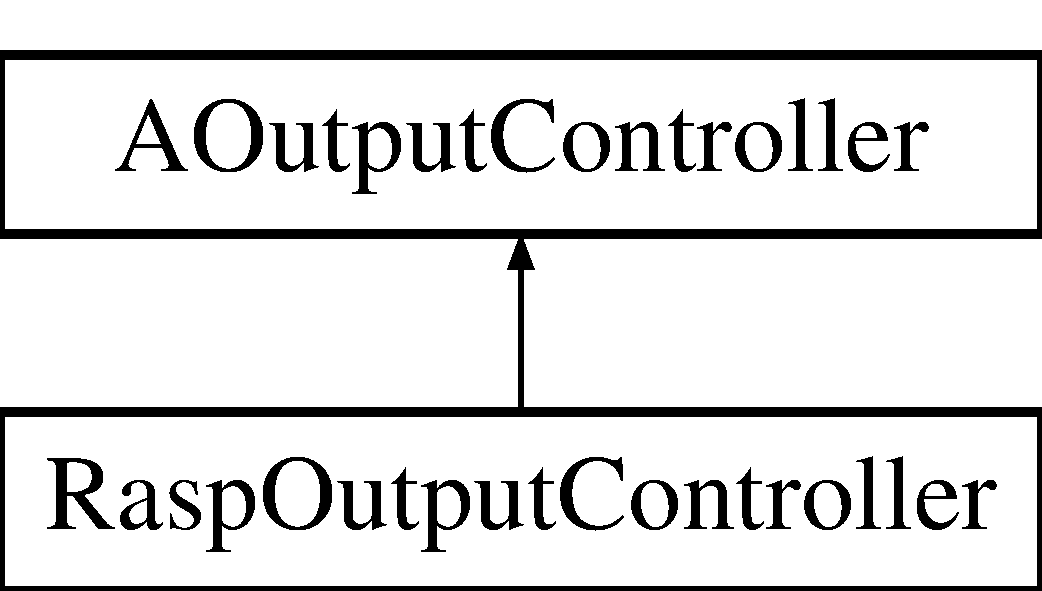
\includegraphics[height=2.000000cm]{class_a_output_controller}
\end{center}
\end{figure}
\subsection*{Öffentliche Methoden}
\begin{DoxyCompactItemize}
\item 
virtual void \hyperlink{class_a_output_controller_a5a818a40e2911411d378032b8b2fb6c8}{position\+Change} (unsigned short new\+Position)=0
\item 
virtual void \hyperlink{class_a_output_controller_ac2b87aa6291c38cc65185bf6a37ae300}{active\+Sample\+Change} (unsigned short new\+Active\+Sample, unsigned short old\+Active\+Sample)=0
\item 
virtual void \hyperlink{class_a_output_controller_a7bad658dfc3eb1223ace0c0454130818}{play\+Position\+Change} (vector$<$ unsigned short $>$ \&new\+Play\+Array)=0
\item 
virtual void \hyperlink{class_a_output_controller_a15c1300df5606bf7d4838b41a45c31e3}{play\+Position\+Change} (unsigned short, unsigned short)=0
\item 
virtual void \hyperlink{class_a_output_controller_ac685432fc57d2441ecb548386554d2c9}{set\+Beat\+Duration} (unsigned int beat\+Duration)=0
\item 
virtual void \hyperlink{class_a_output_controller_ace7df9de71110b3615156b9bd06a9349}{show\+Main\+Screen} (unsigned int bpm)=0
\item 
virtual void \hyperlink{class_a_output_controller_aab53d12a6aa6f38d0e4ead69e85ed4fe}{show\+Sample\+Screen} (unsigned int bpm, float volume)=0
\end{DoxyCompactItemize}


\subsection{Ausführliche Beschreibung}


Definiert in Zeile 8 der Datei A\+Output\+Controller.\+h.



\subsection{Dokumentation der Elementfunktionen}
\mbox{\Hypertarget{class_a_output_controller_ac2b87aa6291c38cc65185bf6a37ae300}\label{class_a_output_controller_ac2b87aa6291c38cc65185bf6a37ae300}} 
\index{A\+Output\+Controller@{A\+Output\+Controller}!active\+Sample\+Change@{active\+Sample\+Change}}
\index{active\+Sample\+Change@{active\+Sample\+Change}!A\+Output\+Controller@{A\+Output\+Controller}}
\subsubsection{\texorpdfstring{active\+Sample\+Change()}{activeSampleChange()}}
{\footnotesize\ttfamily virtual void A\+Output\+Controller\+::active\+Sample\+Change (\begin{DoxyParamCaption}\item[{unsigned short}]{new\+Active\+Sample,  }\item[{unsigned short}]{old\+Active\+Sample }\end{DoxyParamCaption})\hspace{0.3cm}{\ttfamily [pure virtual]}}



Implementiert in \hyperlink{class_rasp_output_controller_a92954cf26d4dd5f7d8835d1d508302c0}{Rasp\+Output\+Controller}.



Wird benutzt von Drum\+Machine\+::set\+Active\+Sample().

\mbox{\Hypertarget{class_a_output_controller_a7bad658dfc3eb1223ace0c0454130818}\label{class_a_output_controller_a7bad658dfc3eb1223ace0c0454130818}} 
\index{A\+Output\+Controller@{A\+Output\+Controller}!play\+Position\+Change@{play\+Position\+Change}}
\index{play\+Position\+Change@{play\+Position\+Change}!A\+Output\+Controller@{A\+Output\+Controller}}
\subsubsection{\texorpdfstring{play\+Position\+Change()}{playPositionChange()}\hspace{0.1cm}{\footnotesize\ttfamily [1/2]}}
{\footnotesize\ttfamily virtual void A\+Output\+Controller\+::play\+Position\+Change (\begin{DoxyParamCaption}\item[{vector$<$ unsigned short $>$ \&}]{new\+Play\+Array }\end{DoxyParamCaption})\hspace{0.3cm}{\ttfamily [pure virtual]}}



Implementiert in \hyperlink{class_rasp_output_controller_af0304196681872f9c1f6d6f2e2db14a6}{Rasp\+Output\+Controller}.



Wird benutzt von Drum\+Machine\+::set\+Active\+Sample() und Drum\+Machine\+::toggle\+Sample\+At\+Beat().

\mbox{\Hypertarget{class_a_output_controller_a15c1300df5606bf7d4838b41a45c31e3}\label{class_a_output_controller_a15c1300df5606bf7d4838b41a45c31e3}} 
\index{A\+Output\+Controller@{A\+Output\+Controller}!play\+Position\+Change@{play\+Position\+Change}}
\index{play\+Position\+Change@{play\+Position\+Change}!A\+Output\+Controller@{A\+Output\+Controller}}
\subsubsection{\texorpdfstring{play\+Position\+Change()}{playPositionChange()}\hspace{0.1cm}{\footnotesize\ttfamily [2/2]}}
{\footnotesize\ttfamily virtual void A\+Output\+Controller\+::play\+Position\+Change (\begin{DoxyParamCaption}\item[{unsigned}]{short,  }\item[{unsigned}]{short }\end{DoxyParamCaption})\hspace{0.3cm}{\ttfamily [pure virtual]}}



Implementiert in \hyperlink{class_rasp_output_controller_a0778395ee8ec044d04fbfcb2f3b2eb04}{Rasp\+Output\+Controller}.

\mbox{\Hypertarget{class_a_output_controller_a5a818a40e2911411d378032b8b2fb6c8}\label{class_a_output_controller_a5a818a40e2911411d378032b8b2fb6c8}} 
\index{A\+Output\+Controller@{A\+Output\+Controller}!position\+Change@{position\+Change}}
\index{position\+Change@{position\+Change}!A\+Output\+Controller@{A\+Output\+Controller}}
\subsubsection{\texorpdfstring{position\+Change()}{positionChange()}}
{\footnotesize\ttfamily virtual void A\+Output\+Controller\+::position\+Change (\begin{DoxyParamCaption}\item[{unsigned short}]{new\+Position }\end{DoxyParamCaption})\hspace{0.3cm}{\ttfamily [pure virtual]}}



Implementiert in \hyperlink{class_rasp_output_controller_afce87d510c0564567e4250b22639d5e0}{Rasp\+Output\+Controller}.



Wird benutzt von Drum\+Machine\+::start\+Loop().

\mbox{\Hypertarget{class_a_output_controller_ac685432fc57d2441ecb548386554d2c9}\label{class_a_output_controller_ac685432fc57d2441ecb548386554d2c9}} 
\index{A\+Output\+Controller@{A\+Output\+Controller}!set\+Beat\+Duration@{set\+Beat\+Duration}}
\index{set\+Beat\+Duration@{set\+Beat\+Duration}!A\+Output\+Controller@{A\+Output\+Controller}}
\subsubsection{\texorpdfstring{set\+Beat\+Duration()}{setBeatDuration()}}
{\footnotesize\ttfamily virtual void A\+Output\+Controller\+::set\+Beat\+Duration (\begin{DoxyParamCaption}\item[{unsigned int}]{beat\+Duration }\end{DoxyParamCaption})\hspace{0.3cm}{\ttfamily [pure virtual]}}



Implementiert in \hyperlink{class_rasp_output_controller_a5fd551f1aba056356befd71e5bff23f1}{Rasp\+Output\+Controller}.



Wird benutzt von Drum\+Machine\+::set\+B\+P\+M().

\mbox{\Hypertarget{class_a_output_controller_ace7df9de71110b3615156b9bd06a9349}\label{class_a_output_controller_ace7df9de71110b3615156b9bd06a9349}} 
\index{A\+Output\+Controller@{A\+Output\+Controller}!show\+Main\+Screen@{show\+Main\+Screen}}
\index{show\+Main\+Screen@{show\+Main\+Screen}!A\+Output\+Controller@{A\+Output\+Controller}}
\subsubsection{\texorpdfstring{show\+Main\+Screen()}{showMainScreen()}}
{\footnotesize\ttfamily virtual void A\+Output\+Controller\+::show\+Main\+Screen (\begin{DoxyParamCaption}\item[{unsigned int}]{bpm }\end{DoxyParamCaption})\hspace{0.3cm}{\ttfamily [pure virtual]}}



Implementiert in \hyperlink{class_rasp_output_controller_ad195a3d664b7c7e5680cd8949203c1fc}{Rasp\+Output\+Controller}.



Wird benutzt von Drum\+Machine\+::set\+Active\+Sample() und Drum\+Machine\+::set\+B\+P\+M().

\mbox{\Hypertarget{class_a_output_controller_aab53d12a6aa6f38d0e4ead69e85ed4fe}\label{class_a_output_controller_aab53d12a6aa6f38d0e4ead69e85ed4fe}} 
\index{A\+Output\+Controller@{A\+Output\+Controller}!show\+Sample\+Screen@{show\+Sample\+Screen}}
\index{show\+Sample\+Screen@{show\+Sample\+Screen}!A\+Output\+Controller@{A\+Output\+Controller}}
\subsubsection{\texorpdfstring{show\+Sample\+Screen()}{showSampleScreen()}}
{\footnotesize\ttfamily virtual void A\+Output\+Controller\+::show\+Sample\+Screen (\begin{DoxyParamCaption}\item[{unsigned int}]{bpm,  }\item[{float}]{volume }\end{DoxyParamCaption})\hspace{0.3cm}{\ttfamily [pure virtual]}}



Implementiert in \hyperlink{class_rasp_output_controller_a613d3a1d1ceb31875be95e4a4b733fba}{Rasp\+Output\+Controller}.



Wird benutzt von Drum\+Machine\+::increase\+Active\+Sample\+Volume() und Drum\+Machine\+::set\+Active\+Sample().



Die Dokumentation für diese Klasse wurde erzeugt aufgrund der Datei\+:\begin{DoxyCompactItemize}
\item 
\hyperlink{_a_output_controller_8h}{A\+Output\+Controller.\+h}\end{DoxyCompactItemize}

\hypertarget{class_display}{}\section{Display Klassenreferenz}
\label{class_display}\index{Display@{Display}}


{\ttfamily \#include $<$Display.\+h$>$}

\subsection*{Öffentliche Methoden}
\begin{DoxyCompactItemize}
\item 
\hyperlink{class_display_ae972fffea6f7ca1d627ef48c3d841bb3}{Display} ()
\item 
void \hyperlink{class_display_aae248dcbc4c44b911c35918feacaf31a}{show\+Main\+Screen} (unsigned short bpm)
\item 
void \hyperlink{class_display_ae00838dd994556524fb8d86d7e855770}{show\+Sample\+Screen} (unsigned short bpm, float volume)
\end{DoxyCompactItemize}
\subsection*{Private Attribute}
\begin{DoxyCompactItemize}
\item 
Adafruit\+\_\+\+S\+S\+D1306 \hyperlink{class_display_ad8b8ca65d118eb16461932c6630463a1}{display}
\end{DoxyCompactItemize}


\subsection{Ausführliche Beschreibung}
A class that holds information an maintains the functionalaty of an Adafruit S\+S\+D1306 \hyperlink{class_display}{Display} 

Definiert in Zeile 12 der Datei Display.\+h.



\subsection{Beschreibung der Konstruktoren und Destruktoren}
\mbox{\Hypertarget{class_display_ae972fffea6f7ca1d627ef48c3d841bb3}\label{class_display_ae972fffea6f7ca1d627ef48c3d841bb3}} 
\index{Display@{Display}!Display@{Display}}
\index{Display@{Display}!Display@{Display}}
\subsubsection{\texorpdfstring{Display()}{Display()}}
{\footnotesize\ttfamily Display\+::\+Display (\begin{DoxyParamCaption}{ }\end{DoxyParamCaption})}

Constructor 

Definiert in Zeile 3 der Datei Display.\+cpp.



Benutzt display.



\subsection{Dokumentation der Elementfunktionen}
\mbox{\Hypertarget{class_display_aae248dcbc4c44b911c35918feacaf31a}\label{class_display_aae248dcbc4c44b911c35918feacaf31a}} 
\index{Display@{Display}!show\+Main\+Screen@{show\+Main\+Screen}}
\index{show\+Main\+Screen@{show\+Main\+Screen}!Display@{Display}}
\subsubsection{\texorpdfstring{show\+Main\+Screen()}{showMainScreen()}}
{\footnotesize\ttfamily void Display\+::show\+Main\+Screen (\begin{DoxyParamCaption}\item[{unsigned short}]{bpm }\end{DoxyParamCaption})}

Activates the main screen 
\begin{DoxyParams}{Parameter}
{\em bpm} & the speed of the loop, is shown in the display \\
\hline
\end{DoxyParams}


Definiert in Zeile 8 der Datei Display.\+cpp.



Benutzt display.



Wird benutzt von Rasp\+Output\+Controller\+::show\+Main\+Screen().

\mbox{\Hypertarget{class_display_ae00838dd994556524fb8d86d7e855770}\label{class_display_ae00838dd994556524fb8d86d7e855770}} 
\index{Display@{Display}!show\+Sample\+Screen@{show\+Sample\+Screen}}
\index{show\+Sample\+Screen@{show\+Sample\+Screen}!Display@{Display}}
\subsubsection{\texorpdfstring{show\+Sample\+Screen()}{showSampleScreen()}}
{\footnotesize\ttfamily void Display\+::show\+Sample\+Screen (\begin{DoxyParamCaption}\item[{unsigned short}]{bpm,  }\item[{float}]{volume }\end{DoxyParamCaption})}

Activates the sample screen 
\begin{DoxyParams}{Parameter}
{\em bpm} & the speed of the loop, is shown in the display \\
\hline
{\em volume} & the volume of the active sample \\
\hline
\end{DoxyParams}


Definiert in Zeile 18 der Datei Display.\+cpp.



Benutzt display.



Wird benutzt von Rasp\+Output\+Controller\+::show\+Sample\+Screen().



\subsection{Dokumentation der Datenelemente}
\mbox{\Hypertarget{class_display_ad8b8ca65d118eb16461932c6630463a1}\label{class_display_ad8b8ca65d118eb16461932c6630463a1}} 
\index{Display@{Display}!display@{display}}
\index{display@{display}!Display@{Display}}
\subsubsection{\texorpdfstring{display}{display}}
{\footnotesize\ttfamily Adafruit\+\_\+\+S\+S\+D1306 Display\+::display\hspace{0.3cm}{\ttfamily [private]}}



Definiert in Zeile 33 der Datei Display.\+h.



Wird benutzt von Display(), show\+Main\+Screen() und show\+Sample\+Screen().



Die Dokumentation für diese Klasse wurde erzeugt aufgrund der Dateien\+:\begin{DoxyCompactItemize}
\item 
\hyperlink{_display_8h}{Display.\+h}\item 
\hyperlink{_display_8cpp}{Display.\+cpp}\end{DoxyCompactItemize}

\hypertarget{class_drum_machine}{}\section{Drum\+Machine Klassenreferenz}
\label{class_drum_machine}\index{Drum\+Machine@{Drum\+Machine}}


Handles the beat loop and samples including correct timing for the give B\+PM, playing them at the correct beat steps and increasing and decreasing the volume.  




{\ttfamily \#include $<$Drum\+Machine.\+h$>$}

\subsection*{Öffentliche Methoden}
\begin{DoxyCompactItemize}
\item 
\hyperlink{class_drum_machine_acacd501a2615a2f0215c04873860ce98}{Drum\+Machine} (\hyperlink{class_a_output_controller}{A\+Output\+Controller} \&\hyperlink{class_drum_machine_a4a5b4d6cc6e4a3ce2c2893e52fd0e951}{output\+Controller})
\item 
void \hyperlink{class_drum_machine_ac42508031bbf331d41c8004ed663c1c1}{start\+Loop} ()
\item 
void \hyperlink{class_drum_machine_af1564a42f1c2717534a61437617070b3}{stop\+Loop} ()
\item 
void \hyperlink{class_drum_machine_a530ac2c3529492c62a01619786fb3765}{add\+Sample} (\hyperlink{class_sample}{Sample})
\item 
void \hyperlink{class_drum_machine_ab823055aa6c1fa1dd91b1e45f3e66f0f}{increase\+Volume} (float value)
\item 
void \hyperlink{class_drum_machine_a2316557d08fecdaa8936be2562749e95}{increase\+Active\+Sample\+Volume} (float value)
\item 
void \hyperlink{class_drum_machine_adbaa7d80f7aa34f1ca190e163515e3e6}{increase\+Bpm} (unsigned short value)
\item 
void \hyperlink{class_drum_machine_ac34e64779cd419a75628630f71a3041b}{toggle\+Sample\+At\+Beat} (unsigned short beat)
\item 
bool \hyperlink{class_drum_machine_aaa0c2e00a5009b239aac709c37602c7d}{is\+Loop\+Running} ()
\item 
void \hyperlink{class_drum_machine_aac554a614388d11543698f407b0e11e6}{set\+B\+PM} (unsigned short \hyperlink{class_drum_machine_afaa80be4a66f759ab590a5f67f327b67}{bpm})
\item 
unsigned short \hyperlink{class_drum_machine_a9a7a34dca1803071fec5b6687cb98343}{get\+B\+PM} ()
\item 
void \hyperlink{class_drum_machine_a19af9f5fbe3242cee5685f1ede574a26}{set\+Master\+Volume} (float \hyperlink{class_drum_machine_af1401c2a8e1d016ec32c662968e581fd}{volume})
\item 
float \hyperlink{class_drum_machine_a3590f99d021aad35cca24fdcb0f8a246}{get\+Master\+Volume} ()
\item 
void \hyperlink{class_drum_machine_a1b6ff2afd815b9981e8a008c857c1847}{set\+Active\+Sample} (unsigned short new\+Active\+Sample)
\item 
unsigned short \hyperlink{class_drum_machine_ac8ef152a82bbce61bc1e2715c3e476b9}{get\+Active\+Sample} ()
\end{DoxyCompactItemize}
\subsection*{Private Methoden}
\begin{DoxyCompactItemize}
\item 
void \hyperlink{class_drum_machine_a5a42497c3a1f390537b6c12fddab1619}{allocate\+Channels} ()
\begin{DoxyCompactList}\small\item\em Helper function which allocates the audio channels. \end{DoxyCompactList}\item 
void \hyperlink{class_drum_machine_afd65a07ff84b6c7854ddd9ee3a529382}{open\+Audio} ()
\begin{DoxyCompactList}\small\item\em Initializes the audio. \end{DoxyCompactList}\end{DoxyCompactItemize}
\subsection*{Private Attribute}
\begin{DoxyCompactItemize}
\item 
const unsigned short \hyperlink{class_drum_machine_a221c0cd8b5cf3f2342f57ad539d3628a}{M\+I\+N\+\_\+\+B\+PM} = 20
\begin{DoxyCompactList}\small\item\em The lowest value the bpm can be. \end{DoxyCompactList}\item 
const unsigned short \hyperlink{class_drum_machine_a0b64f2e265bb9fc06729090b7e05c005}{M\+A\+X\+\_\+\+B\+PM} = 220
\begin{DoxyCompactList}\small\item\em The highest value the bpm can be. \end{DoxyCompactList}\item 
const unsigned short \hyperlink{class_drum_machine_a54e06658e13970dc7679051e8194f546}{W\+H\+O\+L\+E\+\_\+\+B\+E\+A\+TS} = 4
\begin{DoxyCompactList}\small\item\em The number of whole beats the loop has. \end{DoxyCompactList}\item 
const unsigned short \hyperlink{class_drum_machine_ab4d2056f29b6eb959aa379afcc6b70f0}{B\+E\+A\+T\+S\+\_\+\+P\+E\+R\+\_\+\+W\+H\+O\+L\+E\+\_\+\+B\+E\+AT} = 4
\begin{DoxyCompactList}\small\item\em The number of beats one whole beat has. \end{DoxyCompactList}\item 
const unsigned short \hyperlink{class_drum_machine_a25ff7c6556614ab787a626a5c6ec1683}{T\+O\+T\+A\+L\+\_\+\+B\+E\+A\+TS} = \hyperlink{class_drum_machine_a54e06658e13970dc7679051e8194f546}{W\+H\+O\+L\+E\+\_\+\+B\+E\+A\+TS} $\ast$ \hyperlink{class_drum_machine_ab4d2056f29b6eb959aa379afcc6b70f0}{B\+E\+A\+T\+S\+\_\+\+P\+E\+R\+\_\+\+W\+H\+O\+L\+E\+\_\+\+B\+E\+AT}
\begin{DoxyCompactList}\small\item\em The resulting total beats the loop has. \end{DoxyCompactList}\item 
const unsigned long \hyperlink{class_drum_machine_a847e09081c90dbb33c602506d5adb743}{L\+O\+O\+P\+\_\+\+P\+R\+E\+C\+I\+S\+I\+O\+N\+\_\+\+N\+A\+N\+OS} = 10000
\begin{DoxyCompactList}\small\item\em The precision with which the loop timer runs. \end{DoxyCompactList}\item 
unsigned short \hyperlink{class_drum_machine_afaa80be4a66f759ab590a5f67f327b67}{bpm}
\begin{DoxyCompactList}\small\item\em B\+PM at which the loop runs. \end{DoxyCompactList}\item 
unsigned short \hyperlink{class_drum_machine_a46f20be98c71d1429a473e03bf092df3}{current\+Beat}
\begin{DoxyCompactList}\small\item\em The number of the current beat. \end{DoxyCompactList}\item 
unsigned short \hyperlink{class_drum_machine_a9e12916e5724251791689e6f14c8513a}{active\+Sample}
\begin{DoxyCompactList}\small\item\em The index of the active sample. \end{DoxyCompactList}\item 
unsigned int \hyperlink{class_drum_machine_a91179ac48de4159d04052291ad25fa02}{beat\+Millis}
\begin{DoxyCompactList}\small\item\em Milliseconds that one beat lasts. \end{DoxyCompactList}\item 
bool \hyperlink{class_drum_machine_a4ac5a8c113e5a32a557f069e8d93cca8}{loop\+Running}
\begin{DoxyCompactList}\small\item\em Stores whether the loop is running or not. \end{DoxyCompactList}\item 
float \hyperlink{class_drum_machine_af1401c2a8e1d016ec32c662968e581fd}{volume}
\begin{DoxyCompactList}\small\item\em The current master volume. \end{DoxyCompactList}\item 
\hyperlink{class_a_output_controller}{A\+Output\+Controller} \& \hyperlink{class_drum_machine_a4a5b4d6cc6e4a3ce2c2893e52fd0e951}{output\+Controller}
\begin{DoxyCompactList}\small\item\em Reference to the regsitered Output\+Controller. \end{DoxyCompactList}\item 
\hyperlink{class_timer}{Timer} \hyperlink{class_drum_machine_ab190b1b114840e3fb41fff54d0099e93}{loop}
\begin{DoxyCompactList}\small\item\em The loop timer. \end{DoxyCompactList}\item 
vector$<$ \hyperlink{class_sample}{Sample} $>$ \hyperlink{class_drum_machine_acf215ead70c41e760556497281aa562e}{samples}
\begin{DoxyCompactList}\small\item\em A List of all added samples. \end{DoxyCompactList}\end{DoxyCompactItemize}


\subsection{Ausführliche Beschreibung}
Handles the beat loop and samples including correct timing for the give B\+PM, playing them at the correct beat steps and increasing and decreasing the volume. 

Definiert in Zeile 29 der Datei Drum\+Machine.\+h.



\subsection{Beschreibung der Konstruktoren und Destruktoren}
\mbox{\Hypertarget{class_drum_machine_acacd501a2615a2f0215c04873860ce98}\label{class_drum_machine_acacd501a2615a2f0215c04873860ce98}} 
\index{Drum\+Machine@{Drum\+Machine}!Drum\+Machine@{Drum\+Machine}}
\index{Drum\+Machine@{Drum\+Machine}!Drum\+Machine@{Drum\+Machine}}
\subsubsection{\texorpdfstring{Drum\+Machine()}{DrumMachine()}}
{\footnotesize\ttfamily Drum\+Machine\+::\+Drum\+Machine (\begin{DoxyParamCaption}\item[{\hyperlink{class_a_output_controller}{A\+Output\+Controller} \&}]{output\+Controller }\end{DoxyParamCaption})\hspace{0.3cm}{\ttfamily [explicit]}}

Constructor 
\begin{DoxyParams}{Parameter}
{\em output\+Controller} & the output\+Controller the drum machine passes events to \\
\hline
\end{DoxyParams}


Definiert in Zeile 10 der Datei Drum\+Machine.\+cpp.



Benutzt allocate\+Channels() und open\+Audio().



\subsection{Dokumentation der Elementfunktionen}
\mbox{\Hypertarget{class_drum_machine_a530ac2c3529492c62a01619786fb3765}\label{class_drum_machine_a530ac2c3529492c62a01619786fb3765}} 
\index{Drum\+Machine@{Drum\+Machine}!add\+Sample@{add\+Sample}}
\index{add\+Sample@{add\+Sample}!Drum\+Machine@{Drum\+Machine}}
\subsubsection{\texorpdfstring{add\+Sample()}{addSample()}}
{\footnotesize\ttfamily void Drum\+Machine\+::add\+Sample (\begin{DoxyParamCaption}\item[{\hyperlink{class_sample}{Sample}}]{sample }\end{DoxyParamCaption})}

Add a sample to be available for use in the drum machine. The order of adding samples determines the buttons they are mapped to 

Definiert in Zeile 122 der Datei Drum\+Machine.\+cpp.



Benutzt samples, Sample\+::set\+Master\+Volume() und volume.



Wird benutzt von setup().

\mbox{\Hypertarget{class_drum_machine_a5a42497c3a1f390537b6c12fddab1619}\label{class_drum_machine_a5a42497c3a1f390537b6c12fddab1619}} 
\index{Drum\+Machine@{Drum\+Machine}!allocate\+Channels@{allocate\+Channels}}
\index{allocate\+Channels@{allocate\+Channels}!Drum\+Machine@{Drum\+Machine}}
\subsubsection{\texorpdfstring{allocate\+Channels()}{allocateChannels()}}
{\footnotesize\ttfamily void Drum\+Machine\+::allocate\+Channels (\begin{DoxyParamCaption}{ }\end{DoxyParamCaption})\hspace{0.3cm}{\ttfamily [private]}}



Helper function which allocates the audio channels. 



Definiert in Zeile 29 der Datei Drum\+Machine.\+cpp.



Wird benutzt von Drum\+Machine().

\mbox{\Hypertarget{class_drum_machine_ac8ef152a82bbce61bc1e2715c3e476b9}\label{class_drum_machine_ac8ef152a82bbce61bc1e2715c3e476b9}} 
\index{Drum\+Machine@{Drum\+Machine}!get\+Active\+Sample@{get\+Active\+Sample}}
\index{get\+Active\+Sample@{get\+Active\+Sample}!Drum\+Machine@{Drum\+Machine}}
\subsubsection{\texorpdfstring{get\+Active\+Sample()}{getActiveSample()}}
{\footnotesize\ttfamily unsigned short Drum\+Machine\+::get\+Active\+Sample (\begin{DoxyParamCaption}{ }\end{DoxyParamCaption})}

\begin{DoxyReturn}{Rückgabe}
The number of the currently active sample 
\end{DoxyReturn}


Definiert in Zeile 166 der Datei Drum\+Machine.\+cpp.



Benutzt active\+Sample.



Wird benutzt von Drum\+Machine\+Input\+Listener\+::input\+Event().

\mbox{\Hypertarget{class_drum_machine_a9a7a34dca1803071fec5b6687cb98343}\label{class_drum_machine_a9a7a34dca1803071fec5b6687cb98343}} 
\index{Drum\+Machine@{Drum\+Machine}!get\+B\+PM@{get\+B\+PM}}
\index{get\+B\+PM@{get\+B\+PM}!Drum\+Machine@{Drum\+Machine}}
\subsubsection{\texorpdfstring{get\+B\+P\+M()}{getBPM()}}
{\footnotesize\ttfamily unsigned short Drum\+Machine\+::get\+B\+PM (\begin{DoxyParamCaption}{ }\end{DoxyParamCaption})}

\begin{DoxyReturn}{Rückgabe}
the current B\+PM 
\end{DoxyReturn}


Definiert in Zeile 101 der Datei Drum\+Machine.\+cpp.



Benutzt bpm.



Wird benutzt von increase\+Active\+Sample\+Volume(), increase\+Bpm(), Drum\+Machine\+Input\+Listener\+::input\+Event() und set\+Active\+Sample().

\mbox{\Hypertarget{class_drum_machine_a3590f99d021aad35cca24fdcb0f8a246}\label{class_drum_machine_a3590f99d021aad35cca24fdcb0f8a246}} 
\index{Drum\+Machine@{Drum\+Machine}!get\+Master\+Volume@{get\+Master\+Volume}}
\index{get\+Master\+Volume@{get\+Master\+Volume}!Drum\+Machine@{Drum\+Machine}}
\subsubsection{\texorpdfstring{get\+Master\+Volume()}{getMasterVolume()}}
{\footnotesize\ttfamily float Drum\+Machine\+::get\+Master\+Volume (\begin{DoxyParamCaption}{ }\end{DoxyParamCaption})}

\begin{DoxyReturn}{Rückgabe}
the current master volume 
\end{DoxyReturn}


Definiert in Zeile 118 der Datei Drum\+Machine.\+cpp.



Benutzt volume.



Wird benutzt von Drum\+Machine\+Input\+Listener\+::input\+Event().

\mbox{\Hypertarget{class_drum_machine_a2316557d08fecdaa8936be2562749e95}\label{class_drum_machine_a2316557d08fecdaa8936be2562749e95}} 
\index{Drum\+Machine@{Drum\+Machine}!increase\+Active\+Sample\+Volume@{increase\+Active\+Sample\+Volume}}
\index{increase\+Active\+Sample\+Volume@{increase\+Active\+Sample\+Volume}!Drum\+Machine@{Drum\+Machine}}
\subsubsection{\texorpdfstring{increase\+Active\+Sample\+Volume()}{increaseActiveSampleVolume()}}
{\footnotesize\ttfamily void Drum\+Machine\+::increase\+Active\+Sample\+Volume (\begin{DoxyParamCaption}\item[{float}]{value }\end{DoxyParamCaption})}

Increases the volume of the currently active sample by a given value. 
\begin{DoxyParams}{Parameter}
{\em value} & value to increase the active sample volume by \\
\hline
\end{DoxyParams}


Definiert in Zeile 77 der Datei Drum\+Machine.\+cpp.



Benutzt active\+Sample, get\+B\+P\+M(), output\+Controller, samples und A\+Output\+Controller\+::show\+Sample\+Screen().



Wird benutzt von Drum\+Machine\+Input\+Listener\+::input\+Event().

\mbox{\Hypertarget{class_drum_machine_adbaa7d80f7aa34f1ca190e163515e3e6}\label{class_drum_machine_adbaa7d80f7aa34f1ca190e163515e3e6}} 
\index{Drum\+Machine@{Drum\+Machine}!increase\+Bpm@{increase\+Bpm}}
\index{increase\+Bpm@{increase\+Bpm}!Drum\+Machine@{Drum\+Machine}}
\subsubsection{\texorpdfstring{increase\+Bpm()}{increaseBpm()}}
{\footnotesize\ttfamily void Drum\+Machine\+::increase\+Bpm (\begin{DoxyParamCaption}\item[{unsigned short}]{value }\end{DoxyParamCaption})}

Increases the B\+PM by a given value. 
\begin{DoxyParams}{Parameter}
{\em value} & value to increase the bpm by \\
\hline
\end{DoxyParams}


Definiert in Zeile 170 der Datei Drum\+Machine.\+cpp.



Benutzt get\+B\+P\+M() und set\+B\+P\+M().



Wird benutzt von Drum\+Machine\+Input\+Listener\+::input\+Event().

\mbox{\Hypertarget{class_drum_machine_ab823055aa6c1fa1dd91b1e45f3e66f0f}\label{class_drum_machine_ab823055aa6c1fa1dd91b1e45f3e66f0f}} 
\index{Drum\+Machine@{Drum\+Machine}!increase\+Volume@{increase\+Volume}}
\index{increase\+Volume@{increase\+Volume}!Drum\+Machine@{Drum\+Machine}}
\subsubsection{\texorpdfstring{increase\+Volume()}{increaseVolume()}}
{\footnotesize\ttfamily void Drum\+Machine\+::increase\+Volume (\begin{DoxyParamCaption}\item[{float}]{value }\end{DoxyParamCaption})}

Increases the volume by a given value. 
\begin{DoxyParams}{Parameter}
{\em value} & value to increase the master volume by \\
\hline
\end{DoxyParams}


Definiert in Zeile 67 der Datei Drum\+Machine.\+cpp.



Benutzt set\+Master\+Volume() und volume.

\mbox{\Hypertarget{class_drum_machine_aaa0c2e00a5009b239aac709c37602c7d}\label{class_drum_machine_aaa0c2e00a5009b239aac709c37602c7d}} 
\index{Drum\+Machine@{Drum\+Machine}!is\+Loop\+Running@{is\+Loop\+Running}}
\index{is\+Loop\+Running@{is\+Loop\+Running}!Drum\+Machine@{Drum\+Machine}}
\subsubsection{\texorpdfstring{is\+Loop\+Running()}{isLoopRunning()}}
{\footnotesize\ttfamily bool Drum\+Machine\+::is\+Loop\+Running (\begin{DoxyParamCaption}{ }\end{DoxyParamCaption})}

\begin{DoxyReturn}{Rückgabe}
whether the loop is currently running 
\end{DoxyReturn}


Definiert in Zeile 127 der Datei Drum\+Machine.\+cpp.



Benutzt loop\+Running.



Wird benutzt von Drum\+Machine\+Input\+Listener\+::input\+Event().

\mbox{\Hypertarget{class_drum_machine_afd65a07ff84b6c7854ddd9ee3a529382}\label{class_drum_machine_afd65a07ff84b6c7854ddd9ee3a529382}} 
\index{Drum\+Machine@{Drum\+Machine}!open\+Audio@{open\+Audio}}
\index{open\+Audio@{open\+Audio}!Drum\+Machine@{Drum\+Machine}}
\subsubsection{\texorpdfstring{open\+Audio()}{openAudio()}}
{\footnotesize\ttfamily void Drum\+Machine\+::open\+Audio (\begin{DoxyParamCaption}{ }\end{DoxyParamCaption})\hspace{0.3cm}{\ttfamily [private]}}



Initializes the audio. 



Definiert in Zeile 19 der Datei Drum\+Machine.\+cpp.



Wird benutzt von Drum\+Machine().

\mbox{\Hypertarget{class_drum_machine_a1b6ff2afd815b9981e8a008c857c1847}\label{class_drum_machine_a1b6ff2afd815b9981e8a008c857c1847}} 
\index{Drum\+Machine@{Drum\+Machine}!set\+Active\+Sample@{set\+Active\+Sample}}
\index{set\+Active\+Sample@{set\+Active\+Sample}!Drum\+Machine@{Drum\+Machine}}
\subsubsection{\texorpdfstring{set\+Active\+Sample()}{setActiveSample()}}
{\footnotesize\ttfamily void Drum\+Machine\+::set\+Active\+Sample (\begin{DoxyParamCaption}\item[{unsigned short}]{new\+Active\+Sample }\end{DoxyParamCaption})}

Sets the active sample 
\begin{DoxyParams}{Parameter}
{\em new\+Active\+Sample} & The number of the new active sample \\
\hline
\end{DoxyParams}


Definiert in Zeile 131 der Datei Drum\+Machine.\+cpp.



Benutzt active\+Sample, A\+Output\+Controller\+::active\+Sample\+Change(), get\+B\+P\+M(), sample\+::\+N\+O\+\_\+\+S\+A\+M\+P\+LE, output\+Controller, A\+Output\+Controller\+::play\+Position\+Change(), samples, A\+Output\+Controller\+::show\+Main\+Screen() und A\+Output\+Controller\+::show\+Sample\+Screen().



Wird benutzt von Drum\+Machine\+Input\+Listener\+::input\+Event().

\mbox{\Hypertarget{class_drum_machine_aac554a614388d11543698f407b0e11e6}\label{class_drum_machine_aac554a614388d11543698f407b0e11e6}} 
\index{Drum\+Machine@{Drum\+Machine}!set\+B\+PM@{set\+B\+PM}}
\index{set\+B\+PM@{set\+B\+PM}!Drum\+Machine@{Drum\+Machine}}
\subsubsection{\texorpdfstring{set\+B\+P\+M()}{setBPM()}}
{\footnotesize\ttfamily void Drum\+Machine\+::set\+B\+PM (\begin{DoxyParamCaption}\item[{unsigned short}]{bpm }\end{DoxyParamCaption})}

Sets the B\+PM to a specific value 
\begin{DoxyParams}{Parameter}
{\em bpm} & the new bpm value \\
\hline
\end{DoxyParams}


Definiert in Zeile 89 der Datei Drum\+Machine.\+cpp.



Benutzt beat\+Millis, B\+E\+A\+T\+S\+\_\+\+P\+E\+R\+\_\+\+W\+H\+O\+L\+E\+\_\+\+B\+E\+AT, bpm, loop, M\+A\+X\+\_\+\+B\+PM, M\+I\+N\+\_\+\+B\+PM, output\+Controller, A\+Output\+Controller\+::set\+Beat\+Duration(), Timer\+::set\+Interval() und A\+Output\+Controller\+::show\+Main\+Screen().



Wird benutzt von increase\+Bpm() und setup().

\mbox{\Hypertarget{class_drum_machine_a19af9f5fbe3242cee5685f1ede574a26}\label{class_drum_machine_a19af9f5fbe3242cee5685f1ede574a26}} 
\index{Drum\+Machine@{Drum\+Machine}!set\+Master\+Volume@{set\+Master\+Volume}}
\index{set\+Master\+Volume@{set\+Master\+Volume}!Drum\+Machine@{Drum\+Machine}}
\subsubsection{\texorpdfstring{set\+Master\+Volume()}{setMasterVolume()}}
{\footnotesize\ttfamily void Drum\+Machine\+::set\+Master\+Volume (\begin{DoxyParamCaption}\item[{float}]{volume }\end{DoxyParamCaption})}

Sets the master volume to a specific value 
\begin{DoxyParams}{Parameter}
{\em volume} & the new master volume \\
\hline
\end{DoxyParams}


Definiert in Zeile 105 der Datei Drum\+Machine.\+cpp.



Benutzt samples und volume.



Wird benutzt von increase\+Volume().

\mbox{\Hypertarget{class_drum_machine_ac42508031bbf331d41c8004ed663c1c1}\label{class_drum_machine_ac42508031bbf331d41c8004ed663c1c1}} 
\index{Drum\+Machine@{Drum\+Machine}!start\+Loop@{start\+Loop}}
\index{start\+Loop@{start\+Loop}!Drum\+Machine@{Drum\+Machine}}
\subsubsection{\texorpdfstring{start\+Loop()}{startLoop()}}
{\footnotesize\ttfamily void Drum\+Machine\+::start\+Loop (\begin{DoxyParamCaption}{ }\end{DoxyParamCaption})}

Starts the beat loop. 

Definiert in Zeile 37 der Datei Drum\+Machine.\+cpp.



Benutzt beat\+Millis, current\+Beat, loop, loop\+Running, output\+Controller, A\+Output\+Controller\+::position\+Change(), samples, Timer\+::set\+Interval(), Timer\+::start() und T\+O\+T\+A\+L\+\_\+\+B\+E\+A\+TS.



Wird benutzt von Drum\+Machine\+Input\+Listener\+::input\+Event().

\mbox{\Hypertarget{class_drum_machine_af1564a42f1c2717534a61437617070b3}\label{class_drum_machine_af1564a42f1c2717534a61437617070b3}} 
\index{Drum\+Machine@{Drum\+Machine}!stop\+Loop@{stop\+Loop}}
\index{stop\+Loop@{stop\+Loop}!Drum\+Machine@{Drum\+Machine}}
\subsubsection{\texorpdfstring{stop\+Loop()}{stopLoop()}}
{\footnotesize\ttfamily void Drum\+Machine\+::stop\+Loop (\begin{DoxyParamCaption}{ }\end{DoxyParamCaption})}

Stops the beat loop. 

Definiert in Zeile 61 der Datei Drum\+Machine.\+cpp.



Benutzt current\+Beat, loop, loop\+Running und Timer\+::stop().



Wird benutzt von Drum\+Machine\+Input\+Listener\+::input\+Event().

\mbox{\Hypertarget{class_drum_machine_ac34e64779cd419a75628630f71a3041b}\label{class_drum_machine_ac34e64779cd419a75628630f71a3041b}} 
\index{Drum\+Machine@{Drum\+Machine}!toggle\+Sample\+At\+Beat@{toggle\+Sample\+At\+Beat}}
\index{toggle\+Sample\+At\+Beat@{toggle\+Sample\+At\+Beat}!Drum\+Machine@{Drum\+Machine}}
\subsubsection{\texorpdfstring{toggle\+Sample\+At\+Beat()}{toggleSampleAtBeat()}}
{\footnotesize\ttfamily void Drum\+Machine\+::toggle\+Sample\+At\+Beat (\begin{DoxyParamCaption}\item[{unsigned short}]{beat }\end{DoxyParamCaption})}

Toggles whether the current sample is played at a specific beat 
\begin{DoxyParams}{Parameter}
{\em beat} & the beat the sample should be toggled at \\
\hline
\end{DoxyParams}


Definiert in Zeile 152 der Datei Drum\+Machine.\+cpp.



Benutzt active\+Sample, sample\+::\+N\+O\+\_\+\+S\+A\+M\+P\+LE, output\+Controller, A\+Output\+Controller\+::play\+Position\+Change() und samples.



Wird benutzt von Drum\+Machine\+Input\+Listener\+::input\+Event().



\subsection{Dokumentation der Datenelemente}
\mbox{\Hypertarget{class_drum_machine_a9e12916e5724251791689e6f14c8513a}\label{class_drum_machine_a9e12916e5724251791689e6f14c8513a}} 
\index{Drum\+Machine@{Drum\+Machine}!active\+Sample@{active\+Sample}}
\index{active\+Sample@{active\+Sample}!Drum\+Machine@{Drum\+Machine}}
\subsubsection{\texorpdfstring{active\+Sample}{activeSample}}
{\footnotesize\ttfamily unsigned short Drum\+Machine\+::active\+Sample\hspace{0.3cm}{\ttfamily [private]}}



The index of the active sample. 



Definiert in Zeile 40 der Datei Drum\+Machine.\+h.



Wird benutzt von get\+Active\+Sample(), increase\+Active\+Sample\+Volume(), set\+Active\+Sample() und toggle\+Sample\+At\+Beat().

\mbox{\Hypertarget{class_drum_machine_a91179ac48de4159d04052291ad25fa02}\label{class_drum_machine_a91179ac48de4159d04052291ad25fa02}} 
\index{Drum\+Machine@{Drum\+Machine}!beat\+Millis@{beat\+Millis}}
\index{beat\+Millis@{beat\+Millis}!Drum\+Machine@{Drum\+Machine}}
\subsubsection{\texorpdfstring{beat\+Millis}{beatMillis}}
{\footnotesize\ttfamily unsigned int Drum\+Machine\+::beat\+Millis\hspace{0.3cm}{\ttfamily [private]}}



Milliseconds that one beat lasts. 



Definiert in Zeile 41 der Datei Drum\+Machine.\+h.



Wird benutzt von set\+B\+P\+M() und start\+Loop().

\mbox{\Hypertarget{class_drum_machine_ab4d2056f29b6eb959aa379afcc6b70f0}\label{class_drum_machine_ab4d2056f29b6eb959aa379afcc6b70f0}} 
\index{Drum\+Machine@{Drum\+Machine}!B\+E\+A\+T\+S\+\_\+\+P\+E\+R\+\_\+\+W\+H\+O\+L\+E\+\_\+\+B\+E\+AT@{B\+E\+A\+T\+S\+\_\+\+P\+E\+R\+\_\+\+W\+H\+O\+L\+E\+\_\+\+B\+E\+AT}}
\index{B\+E\+A\+T\+S\+\_\+\+P\+E\+R\+\_\+\+W\+H\+O\+L\+E\+\_\+\+B\+E\+AT@{B\+E\+A\+T\+S\+\_\+\+P\+E\+R\+\_\+\+W\+H\+O\+L\+E\+\_\+\+B\+E\+AT}!Drum\+Machine@{Drum\+Machine}}
\subsubsection{\texorpdfstring{B\+E\+A\+T\+S\+\_\+\+P\+E\+R\+\_\+\+W\+H\+O\+L\+E\+\_\+\+B\+E\+AT}{BEATS\_PER\_WHOLE\_BEAT}}
{\footnotesize\ttfamily const unsigned short Drum\+Machine\+::\+B\+E\+A\+T\+S\+\_\+\+P\+E\+R\+\_\+\+W\+H\+O\+L\+E\+\_\+\+B\+E\+AT = 4\hspace{0.3cm}{\ttfamily [private]}}



The number of beats one whole beat has. 



Definiert in Zeile 34 der Datei Drum\+Machine.\+h.



Wird benutzt von set\+B\+P\+M().

\mbox{\Hypertarget{class_drum_machine_afaa80be4a66f759ab590a5f67f327b67}\label{class_drum_machine_afaa80be4a66f759ab590a5f67f327b67}} 
\index{Drum\+Machine@{Drum\+Machine}!bpm@{bpm}}
\index{bpm@{bpm}!Drum\+Machine@{Drum\+Machine}}
\subsubsection{\texorpdfstring{bpm}{bpm}}
{\footnotesize\ttfamily unsigned short Drum\+Machine\+::bpm\hspace{0.3cm}{\ttfamily [private]}}



B\+PM at which the loop runs. 



Definiert in Zeile 38 der Datei Drum\+Machine.\+h.



Wird benutzt von get\+B\+P\+M() und set\+B\+P\+M().

\mbox{\Hypertarget{class_drum_machine_a46f20be98c71d1429a473e03bf092df3}\label{class_drum_machine_a46f20be98c71d1429a473e03bf092df3}} 
\index{Drum\+Machine@{Drum\+Machine}!current\+Beat@{current\+Beat}}
\index{current\+Beat@{current\+Beat}!Drum\+Machine@{Drum\+Machine}}
\subsubsection{\texorpdfstring{current\+Beat}{currentBeat}}
{\footnotesize\ttfamily unsigned short Drum\+Machine\+::current\+Beat\hspace{0.3cm}{\ttfamily [private]}}



The number of the current beat. 



Definiert in Zeile 39 der Datei Drum\+Machine.\+h.



Wird benutzt von start\+Loop() und stop\+Loop().

\mbox{\Hypertarget{class_drum_machine_ab190b1b114840e3fb41fff54d0099e93}\label{class_drum_machine_ab190b1b114840e3fb41fff54d0099e93}} 
\index{Drum\+Machine@{Drum\+Machine}!loop@{loop}}
\index{loop@{loop}!Drum\+Machine@{Drum\+Machine}}
\subsubsection{\texorpdfstring{loop}{loop}}
{\footnotesize\ttfamily \hyperlink{class_timer}{Timer} Drum\+Machine\+::loop\hspace{0.3cm}{\ttfamily [private]}}



The loop timer. 



Definiert in Zeile 46 der Datei Drum\+Machine.\+h.



Wird benutzt von set\+B\+P\+M(), start\+Loop() und stop\+Loop().

\mbox{\Hypertarget{class_drum_machine_a847e09081c90dbb33c602506d5adb743}\label{class_drum_machine_a847e09081c90dbb33c602506d5adb743}} 
\index{Drum\+Machine@{Drum\+Machine}!L\+O\+O\+P\+\_\+\+P\+R\+E\+C\+I\+S\+I\+O\+N\+\_\+\+N\+A\+N\+OS@{L\+O\+O\+P\+\_\+\+P\+R\+E\+C\+I\+S\+I\+O\+N\+\_\+\+N\+A\+N\+OS}}
\index{L\+O\+O\+P\+\_\+\+P\+R\+E\+C\+I\+S\+I\+O\+N\+\_\+\+N\+A\+N\+OS@{L\+O\+O\+P\+\_\+\+P\+R\+E\+C\+I\+S\+I\+O\+N\+\_\+\+N\+A\+N\+OS}!Drum\+Machine@{Drum\+Machine}}
\subsubsection{\texorpdfstring{L\+O\+O\+P\+\_\+\+P\+R\+E\+C\+I\+S\+I\+O\+N\+\_\+\+N\+A\+N\+OS}{LOOP\_PRECISION\_NANOS}}
{\footnotesize\ttfamily const unsigned long Drum\+Machine\+::\+L\+O\+O\+P\+\_\+\+P\+R\+E\+C\+I\+S\+I\+O\+N\+\_\+\+N\+A\+N\+OS = 10000\hspace{0.3cm}{\ttfamily [private]}}



The precision with which the loop timer runs. 



Definiert in Zeile 36 der Datei Drum\+Machine.\+h.

\mbox{\Hypertarget{class_drum_machine_a4ac5a8c113e5a32a557f069e8d93cca8}\label{class_drum_machine_a4ac5a8c113e5a32a557f069e8d93cca8}} 
\index{Drum\+Machine@{Drum\+Machine}!loop\+Running@{loop\+Running}}
\index{loop\+Running@{loop\+Running}!Drum\+Machine@{Drum\+Machine}}
\subsubsection{\texorpdfstring{loop\+Running}{loopRunning}}
{\footnotesize\ttfamily bool Drum\+Machine\+::loop\+Running\hspace{0.3cm}{\ttfamily [private]}}



Stores whether the loop is running or not. 



Definiert in Zeile 42 der Datei Drum\+Machine.\+h.



Wird benutzt von is\+Loop\+Running(), start\+Loop() und stop\+Loop().

\mbox{\Hypertarget{class_drum_machine_a0b64f2e265bb9fc06729090b7e05c005}\label{class_drum_machine_a0b64f2e265bb9fc06729090b7e05c005}} 
\index{Drum\+Machine@{Drum\+Machine}!M\+A\+X\+\_\+\+B\+PM@{M\+A\+X\+\_\+\+B\+PM}}
\index{M\+A\+X\+\_\+\+B\+PM@{M\+A\+X\+\_\+\+B\+PM}!Drum\+Machine@{Drum\+Machine}}
\subsubsection{\texorpdfstring{M\+A\+X\+\_\+\+B\+PM}{MAX\_BPM}}
{\footnotesize\ttfamily const unsigned short Drum\+Machine\+::\+M\+A\+X\+\_\+\+B\+PM = 220\hspace{0.3cm}{\ttfamily [private]}}



The highest value the bpm can be. 



Definiert in Zeile 32 der Datei Drum\+Machine.\+h.



Wird benutzt von set\+B\+P\+M().

\mbox{\Hypertarget{class_drum_machine_a221c0cd8b5cf3f2342f57ad539d3628a}\label{class_drum_machine_a221c0cd8b5cf3f2342f57ad539d3628a}} 
\index{Drum\+Machine@{Drum\+Machine}!M\+I\+N\+\_\+\+B\+PM@{M\+I\+N\+\_\+\+B\+PM}}
\index{M\+I\+N\+\_\+\+B\+PM@{M\+I\+N\+\_\+\+B\+PM}!Drum\+Machine@{Drum\+Machine}}
\subsubsection{\texorpdfstring{M\+I\+N\+\_\+\+B\+PM}{MIN\_BPM}}
{\footnotesize\ttfamily const unsigned short Drum\+Machine\+::\+M\+I\+N\+\_\+\+B\+PM = 20\hspace{0.3cm}{\ttfamily [private]}}



The lowest value the bpm can be. 



Definiert in Zeile 31 der Datei Drum\+Machine.\+h.



Wird benutzt von set\+B\+P\+M().

\mbox{\Hypertarget{class_drum_machine_a4a5b4d6cc6e4a3ce2c2893e52fd0e951}\label{class_drum_machine_a4a5b4d6cc6e4a3ce2c2893e52fd0e951}} 
\index{Drum\+Machine@{Drum\+Machine}!output\+Controller@{output\+Controller}}
\index{output\+Controller@{output\+Controller}!Drum\+Machine@{Drum\+Machine}}
\subsubsection{\texorpdfstring{output\+Controller}{outputController}}
{\footnotesize\ttfamily \hyperlink{class_a_output_controller}{A\+Output\+Controller}\& Drum\+Machine\+::output\+Controller\hspace{0.3cm}{\ttfamily [private]}}



Reference to the regsitered Output\+Controller. 



Definiert in Zeile 45 der Datei Drum\+Machine.\+h.



Wird benutzt von increase\+Active\+Sample\+Volume(), set\+Active\+Sample(), set\+B\+P\+M(), start\+Loop() und toggle\+Sample\+At\+Beat().

\mbox{\Hypertarget{class_drum_machine_acf215ead70c41e760556497281aa562e}\label{class_drum_machine_acf215ead70c41e760556497281aa562e}} 
\index{Drum\+Machine@{Drum\+Machine}!samples@{samples}}
\index{samples@{samples}!Drum\+Machine@{Drum\+Machine}}
\subsubsection{\texorpdfstring{samples}{samples}}
{\footnotesize\ttfamily vector$<$\hyperlink{class_sample}{Sample}$>$ Drum\+Machine\+::samples\hspace{0.3cm}{\ttfamily [private]}}



A List of all added samples. 



Definiert in Zeile 47 der Datei Drum\+Machine.\+h.



Wird benutzt von add\+Sample(), increase\+Active\+Sample\+Volume(), set\+Active\+Sample(), set\+Master\+Volume(), start\+Loop() und toggle\+Sample\+At\+Beat().

\mbox{\Hypertarget{class_drum_machine_a25ff7c6556614ab787a626a5c6ec1683}\label{class_drum_machine_a25ff7c6556614ab787a626a5c6ec1683}} 
\index{Drum\+Machine@{Drum\+Machine}!T\+O\+T\+A\+L\+\_\+\+B\+E\+A\+TS@{T\+O\+T\+A\+L\+\_\+\+B\+E\+A\+TS}}
\index{T\+O\+T\+A\+L\+\_\+\+B\+E\+A\+TS@{T\+O\+T\+A\+L\+\_\+\+B\+E\+A\+TS}!Drum\+Machine@{Drum\+Machine}}
\subsubsection{\texorpdfstring{T\+O\+T\+A\+L\+\_\+\+B\+E\+A\+TS}{TOTAL\_BEATS}}
{\footnotesize\ttfamily const unsigned short Drum\+Machine\+::\+T\+O\+T\+A\+L\+\_\+\+B\+E\+A\+TS = \hyperlink{class_drum_machine_a54e06658e13970dc7679051e8194f546}{W\+H\+O\+L\+E\+\_\+\+B\+E\+A\+TS} $\ast$ \hyperlink{class_drum_machine_ab4d2056f29b6eb959aa379afcc6b70f0}{B\+E\+A\+T\+S\+\_\+\+P\+E\+R\+\_\+\+W\+H\+O\+L\+E\+\_\+\+B\+E\+AT}\hspace{0.3cm}{\ttfamily [private]}}



The resulting total beats the loop has. 



Definiert in Zeile 35 der Datei Drum\+Machine.\+h.



Wird benutzt von start\+Loop().

\mbox{\Hypertarget{class_drum_machine_af1401c2a8e1d016ec32c662968e581fd}\label{class_drum_machine_af1401c2a8e1d016ec32c662968e581fd}} 
\index{Drum\+Machine@{Drum\+Machine}!volume@{volume}}
\index{volume@{volume}!Drum\+Machine@{Drum\+Machine}}
\subsubsection{\texorpdfstring{volume}{volume}}
{\footnotesize\ttfamily float Drum\+Machine\+::volume\hspace{0.3cm}{\ttfamily [private]}}



The current master volume. 



Definiert in Zeile 43 der Datei Drum\+Machine.\+h.



Wird benutzt von add\+Sample(), get\+Master\+Volume(), increase\+Volume() und set\+Master\+Volume().

\mbox{\Hypertarget{class_drum_machine_a54e06658e13970dc7679051e8194f546}\label{class_drum_machine_a54e06658e13970dc7679051e8194f546}} 
\index{Drum\+Machine@{Drum\+Machine}!W\+H\+O\+L\+E\+\_\+\+B\+E\+A\+TS@{W\+H\+O\+L\+E\+\_\+\+B\+E\+A\+TS}}
\index{W\+H\+O\+L\+E\+\_\+\+B\+E\+A\+TS@{W\+H\+O\+L\+E\+\_\+\+B\+E\+A\+TS}!Drum\+Machine@{Drum\+Machine}}
\subsubsection{\texorpdfstring{W\+H\+O\+L\+E\+\_\+\+B\+E\+A\+TS}{WHOLE\_BEATS}}
{\footnotesize\ttfamily const unsigned short Drum\+Machine\+::\+W\+H\+O\+L\+E\+\_\+\+B\+E\+A\+TS = 4\hspace{0.3cm}{\ttfamily [private]}}



The number of whole beats the loop has. 



Definiert in Zeile 33 der Datei Drum\+Machine.\+h.



Die Dokumentation für diese Klasse wurde erzeugt aufgrund der Dateien\+:\begin{DoxyCompactItemize}
\item 
\hyperlink{_drum_machine_8h}{Drum\+Machine.\+h}\item 
\hyperlink{_drum_machine_8cpp}{Drum\+Machine.\+cpp}\end{DoxyCompactItemize}

\hypertarget{class_drum_machine_input_listener}{}\section{Drum\+Machine\+Input\+Listener Klassenreferenz}
\label{class_drum_machine_input_listener}\index{Drum\+Machine\+Input\+Listener@{Drum\+Machine\+Input\+Listener}}


{\ttfamily \#include $<$Drum\+Machine\+Input\+Listener.\+h$>$}

Klassendiagramm für Drum\+Machine\+Input\+Listener\+:\begin{figure}[H]
\begin{center}
\leavevmode
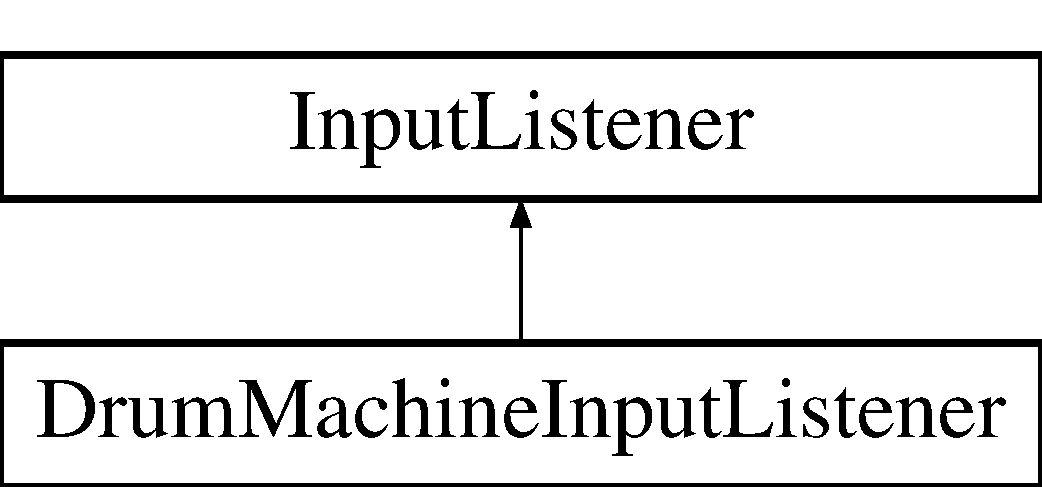
\includegraphics[height=2.000000cm]{class_drum_machine_input_listener}
\end{center}
\end{figure}
\subsection*{Öffentliche Methoden}
\begin{DoxyCompactItemize}
\item 
\hyperlink{class_drum_machine_input_listener_a7552c36ebae9e6ae49f8929ae9853354}{Drum\+Machine\+Input\+Listener} (\hyperlink{class_drum_machine}{Drum\+Machine} \&\hyperlink{class_drum_machine_input_listener_ae3f80aad0a5c4b2e4ad2712423102feb}{drum\+Machine})
\item 
void \hyperlink{class_drum_machine_input_listener_a44a620b09b35885a26befe84fa6e1ab0}{input\+Event} (unsigned short event) override
\end{DoxyCompactItemize}
\subsection*{Private Attribute}
\begin{DoxyCompactItemize}
\item 
const float \hyperlink{class_drum_machine_input_listener_a983e85ff0ebfbb3de0a917134488570c}{V\+O\+L\+U\+M\+E\+\_\+\+S\+T\+E\+P\+\_\+\+S\+I\+ZE} = 0.\+05f
\item 
const unsigned short \hyperlink{class_drum_machine_input_listener_ad4f83d21be6ff1ba703a27d8c9a04c9a}{B\+P\+M\+\_\+\+S\+T\+E\+P\+\_\+\+S\+I\+ZE} = 1
\item 
\hyperlink{class_drum_machine}{Drum\+Machine} \& \hyperlink{class_drum_machine_input_listener_ae3f80aad0a5c4b2e4ad2712423102feb}{drum\+Machine}
\end{DoxyCompactItemize}


\subsection{Ausführliche Beschreibung}


Definiert in Zeile 8 der Datei Drum\+Machine\+Input\+Listener.\+h.



\subsection{Beschreibung der Konstruktoren und Destruktoren}
\mbox{\Hypertarget{class_drum_machine_input_listener_a7552c36ebae9e6ae49f8929ae9853354}\label{class_drum_machine_input_listener_a7552c36ebae9e6ae49f8929ae9853354}} 
\index{Drum\+Machine\+Input\+Listener@{Drum\+Machine\+Input\+Listener}!Drum\+Machine\+Input\+Listener@{Drum\+Machine\+Input\+Listener}}
\index{Drum\+Machine\+Input\+Listener@{Drum\+Machine\+Input\+Listener}!Drum\+Machine\+Input\+Listener@{Drum\+Machine\+Input\+Listener}}
\subsubsection{\texorpdfstring{Drum\+Machine\+Input\+Listener()}{DrumMachineInputListener()}}
{\footnotesize\ttfamily Drum\+Machine\+Input\+Listener\+::\+Drum\+Machine\+Input\+Listener (\begin{DoxyParamCaption}\item[{\hyperlink{class_drum_machine}{Drum\+Machine} \&}]{drum\+Machine }\end{DoxyParamCaption})\hspace{0.3cm}{\ttfamily [explicit]}}



Definiert in Zeile 8 der Datei Drum\+Machine\+Input\+Listener.\+cpp.



\subsection{Dokumentation der Elementfunktionen}
\mbox{\Hypertarget{class_drum_machine_input_listener_a44a620b09b35885a26befe84fa6e1ab0}\label{class_drum_machine_input_listener_a44a620b09b35885a26befe84fa6e1ab0}} 
\index{Drum\+Machine\+Input\+Listener@{Drum\+Machine\+Input\+Listener}!input\+Event@{input\+Event}}
\index{input\+Event@{input\+Event}!Drum\+Machine\+Input\+Listener@{Drum\+Machine\+Input\+Listener}}
\subsubsection{\texorpdfstring{input\+Event()}{inputEvent()}}
{\footnotesize\ttfamily void Drum\+Machine\+Input\+Listener\+::input\+Event (\begin{DoxyParamCaption}\item[{unsigned short}]{event }\end{DoxyParamCaption})\hspace{0.3cm}{\ttfamily [override]}, {\ttfamily [virtual]}}



Implementiert \hyperlink{class_input_listener_a1a3d74f2ffc108c773511ea4be250f7d}{Input\+Listener}.



Definiert in Zeile 10 der Datei Drum\+Machine\+Input\+Listener.\+cpp.



Benutzt beat\+::\+B\+E\+A\+T1, beat\+::\+B\+E\+A\+T10, inputs\+::\+B\+E\+A\+T10\+\_\+\+B\+U\+T\+T\+ON, beat\+::\+B\+E\+A\+T11, inputs\+::\+B\+E\+A\+T11\+\_\+\+B\+U\+T\+T\+ON, beat\+::\+B\+E\+A\+T12, inputs\+::\+B\+E\+A\+T12\+\_\+\+B\+U\+T\+T\+ON, beat\+::\+B\+E\+A\+T13, inputs\+::\+B\+E\+A\+T13\+\_\+\+B\+U\+T\+T\+ON, beat\+::\+B\+E\+A\+T14, inputs\+::\+B\+E\+A\+T14\+\_\+\+B\+U\+T\+T\+ON, beat\+::\+B\+E\+A\+T15, inputs\+::\+B\+E\+A\+T15\+\_\+\+B\+U\+T\+T\+ON, beat\+::\+B\+E\+A\+T16, inputs\+::\+B\+E\+A\+T16\+\_\+\+B\+U\+T\+T\+ON, inputs\+::\+B\+E\+A\+T1\+\_\+\+B\+U\+T\+T\+ON, beat\+::\+B\+E\+A\+T2, inputs\+::\+B\+E\+A\+T2\+\_\+\+B\+U\+T\+T\+ON, beat\+::\+B\+E\+A\+T3, inputs\+::\+B\+E\+A\+T3\+\_\+\+B\+U\+T\+T\+ON, beat\+::\+B\+E\+A\+T4, inputs\+::\+B\+E\+A\+T4\+\_\+\+B\+U\+T\+T\+ON, beat\+::\+B\+E\+A\+T5, inputs\+::\+B\+E\+A\+T5\+\_\+\+B\+U\+T\+T\+ON, beat\+::\+B\+E\+A\+T6, inputs\+::\+B\+E\+A\+T6\+\_\+\+B\+U\+T\+T\+ON, beat\+::\+B\+E\+A\+T7, inputs\+::\+B\+E\+A\+T7\+\_\+\+B\+U\+T\+T\+ON, beat\+::\+B\+E\+A\+T8, inputs\+::\+B\+E\+A\+T8\+\_\+\+B\+U\+T\+T\+ON, beat\+::\+B\+E\+A\+T9, inputs\+::\+B\+E\+A\+T9\+\_\+\+B\+U\+T\+T\+ON, B\+P\+M\+\_\+\+S\+T\+E\+P\+\_\+\+S\+I\+ZE, drum\+Machine, Drum\+Machine\+::get\+Active\+Sample(), Drum\+Machine\+::get\+B\+P\+M(), Drum\+Machine\+::get\+Master\+Volume(), Drum\+Machine\+::increase\+Active\+Sample\+Volume(), Drum\+Machine\+::increase\+Bpm(), Drum\+Machine\+::is\+Loop\+Running(), sample\+::\+N\+O\+\_\+\+S\+A\+M\+P\+LE, sample\+::\+S\+A\+M\+P\+L\+E1, inputs\+::\+S\+A\+M\+P\+L\+E1\+\_\+\+B\+U\+T\+T\+ON, sample\+::\+S\+A\+M\+P\+L\+E2, inputs\+::\+S\+A\+M\+P\+L\+E2\+\_\+\+B\+U\+T\+T\+ON, sample\+::\+S\+A\+M\+P\+L\+E3, inputs\+::\+S\+A\+M\+P\+L\+E3\+\_\+\+B\+U\+T\+T\+ON, sample\+::\+S\+A\+M\+P\+L\+E4, inputs\+::\+S\+A\+M\+P\+L\+E4\+\_\+\+B\+U\+T\+T\+ON, sample\+::\+S\+A\+M\+P\+L\+E5, inputs\+::\+S\+A\+M\+P\+L\+E5\+\_\+\+B\+U\+T\+T\+ON, sample\+::\+S\+A\+M\+P\+L\+E6, inputs\+::\+S\+A\+M\+P\+L\+E6\+\_\+\+B\+U\+T\+T\+ON, sample\+::\+S\+A\+M\+P\+L\+E7, inputs\+::\+S\+A\+M\+P\+L\+E7\+\_\+\+B\+U\+T\+T\+ON, sample\+::\+S\+A\+M\+P\+L\+E8, inputs\+::\+S\+A\+M\+P\+L\+E8\+\_\+\+B\+U\+T\+T\+ON, Drum\+Machine\+::set\+Active\+Sample(), inputs\+::\+S\+T\+A\+R\+T\+\_\+\+S\+T\+O\+P\+\_\+\+B\+U\+T\+T\+ON, Drum\+Machine\+::start\+Loop(), Drum\+Machine\+::stop\+Loop(), Drum\+Machine\+::toggle\+Sample\+At\+Beat(), inputs\+::\+V\+O\+L\+U\+M\+E\+\_\+\+B\+P\+M\+\_\+\+D\+O\+W\+N\+\_\+\+B\+U\+T\+T\+ON, inputs\+::\+V\+O\+L\+U\+M\+E\+\_\+\+B\+P\+M\+\_\+\+U\+P\+\_\+\+B\+U\+T\+T\+ON und V\+O\+L\+U\+M\+E\+\_\+\+S\+T\+E\+P\+\_\+\+S\+I\+ZE.



\subsection{Dokumentation der Datenelemente}
\mbox{\Hypertarget{class_drum_machine_input_listener_ad4f83d21be6ff1ba703a27d8c9a04c9a}\label{class_drum_machine_input_listener_ad4f83d21be6ff1ba703a27d8c9a04c9a}} 
\index{Drum\+Machine\+Input\+Listener@{Drum\+Machine\+Input\+Listener}!B\+P\+M\+\_\+\+S\+T\+E\+P\+\_\+\+S\+I\+ZE@{B\+P\+M\+\_\+\+S\+T\+E\+P\+\_\+\+S\+I\+ZE}}
\index{B\+P\+M\+\_\+\+S\+T\+E\+P\+\_\+\+S\+I\+ZE@{B\+P\+M\+\_\+\+S\+T\+E\+P\+\_\+\+S\+I\+ZE}!Drum\+Machine\+Input\+Listener@{Drum\+Machine\+Input\+Listener}}
\subsubsection{\texorpdfstring{B\+P\+M\+\_\+\+S\+T\+E\+P\+\_\+\+S\+I\+ZE}{BPM\_STEP\_SIZE}}
{\footnotesize\ttfamily const unsigned short Drum\+Machine\+Input\+Listener\+::\+B\+P\+M\+\_\+\+S\+T\+E\+P\+\_\+\+S\+I\+ZE = 1\hspace{0.3cm}{\ttfamily [private]}}



Definiert in Zeile 11 der Datei Drum\+Machine\+Input\+Listener.\+h.



Wird benutzt von input\+Event().

\mbox{\Hypertarget{class_drum_machine_input_listener_ae3f80aad0a5c4b2e4ad2712423102feb}\label{class_drum_machine_input_listener_ae3f80aad0a5c4b2e4ad2712423102feb}} 
\index{Drum\+Machine\+Input\+Listener@{Drum\+Machine\+Input\+Listener}!drum\+Machine@{drum\+Machine}}
\index{drum\+Machine@{drum\+Machine}!Drum\+Machine\+Input\+Listener@{Drum\+Machine\+Input\+Listener}}
\subsubsection{\texorpdfstring{drum\+Machine}{drumMachine}}
{\footnotesize\ttfamily \hyperlink{class_drum_machine}{Drum\+Machine}\& Drum\+Machine\+Input\+Listener\+::drum\+Machine\hspace{0.3cm}{\ttfamily [private]}}



Definiert in Zeile 13 der Datei Drum\+Machine\+Input\+Listener.\+h.



Wird benutzt von input\+Event().

\mbox{\Hypertarget{class_drum_machine_input_listener_a983e85ff0ebfbb3de0a917134488570c}\label{class_drum_machine_input_listener_a983e85ff0ebfbb3de0a917134488570c}} 
\index{Drum\+Machine\+Input\+Listener@{Drum\+Machine\+Input\+Listener}!V\+O\+L\+U\+M\+E\+\_\+\+S\+T\+E\+P\+\_\+\+S\+I\+ZE@{V\+O\+L\+U\+M\+E\+\_\+\+S\+T\+E\+P\+\_\+\+S\+I\+ZE}}
\index{V\+O\+L\+U\+M\+E\+\_\+\+S\+T\+E\+P\+\_\+\+S\+I\+ZE@{V\+O\+L\+U\+M\+E\+\_\+\+S\+T\+E\+P\+\_\+\+S\+I\+ZE}!Drum\+Machine\+Input\+Listener@{Drum\+Machine\+Input\+Listener}}
\subsubsection{\texorpdfstring{V\+O\+L\+U\+M\+E\+\_\+\+S\+T\+E\+P\+\_\+\+S\+I\+ZE}{VOLUME\_STEP\_SIZE}}
{\footnotesize\ttfamily const float Drum\+Machine\+Input\+Listener\+::\+V\+O\+L\+U\+M\+E\+\_\+\+S\+T\+E\+P\+\_\+\+S\+I\+ZE = 0.\+05f\hspace{0.3cm}{\ttfamily [private]}}



Definiert in Zeile 10 der Datei Drum\+Machine\+Input\+Listener.\+h.



Wird benutzt von input\+Event().



Die Dokumentation für diese Klasse wurde erzeugt aufgrund der Dateien\+:\begin{DoxyCompactItemize}
\item 
\hyperlink{_drum_machine_input_listener_8h}{Drum\+Machine\+Input\+Listener.\+h}\item 
\hyperlink{_drum_machine_input_listener_8cpp}{Drum\+Machine\+Input\+Listener.\+cpp}\end{DoxyCompactItemize}

\hypertarget{class_input_listener}{}\section{Input\+Listener Klassenreferenz}
\label{class_input_listener}\index{Input\+Listener@{Input\+Listener}}


Interface for input listeners to register in the \hyperlink{class_rasp_input_controller}{Rasp\+Input\+Controller}.  




{\ttfamily \#include $<$Input\+Listener.\+h$>$}

Klassendiagramm für Input\+Listener\+:\begin{figure}[H]
\begin{center}
\leavevmode
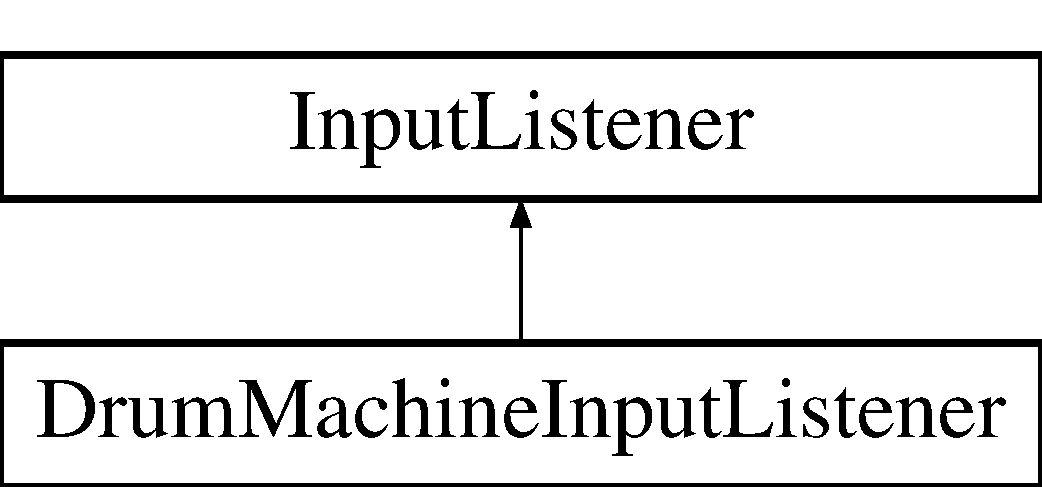
\includegraphics[height=2.000000cm]{class_input_listener}
\end{center}
\end{figure}
\subsection*{Öffentliche Methoden}
\begin{DoxyCompactItemize}
\item 
virtual void \hyperlink{class_input_listener_a1a3d74f2ffc108c773511ea4be250f7d}{input\+Event} (unsigned short input)=0
\end{DoxyCompactItemize}


\subsection{Ausführliche Beschreibung}
Interface for input listeners to register in the \hyperlink{class_rasp_input_controller}{Rasp\+Input\+Controller}. 

Definiert in Zeile 11 der Datei Input\+Listener.\+h.



\subsection{Dokumentation der Elementfunktionen}
\mbox{\Hypertarget{class_input_listener_a1a3d74f2ffc108c773511ea4be250f7d}\label{class_input_listener_a1a3d74f2ffc108c773511ea4be250f7d}} 
\index{Input\+Listener@{Input\+Listener}!input\+Event@{input\+Event}}
\index{input\+Event@{input\+Event}!Input\+Listener@{Input\+Listener}}
\subsubsection{\texorpdfstring{input\+Event()}{inputEvent()}}
{\footnotesize\ttfamily virtual void Input\+Listener\+::input\+Event (\begin{DoxyParamCaption}\item[{unsigned short}]{input }\end{DoxyParamCaption})\hspace{0.3cm}{\ttfamily [pure virtual]}}

Called when new input events are detected 
\begin{DoxyParams}{Parameter}
{\em input} & the input that was detected. \\
\hline
\end{DoxyParams}


Implementiert in \hyperlink{class_drum_machine_input_listener_a44a620b09b35885a26befe84fa6e1ab0}{Drum\+Machine\+Input\+Listener}.



Die Dokumentation für diese Klasse wurde erzeugt aufgrund der Datei\+:\begin{DoxyCompactItemize}
\item 
\hyperlink{_input_listener_8h}{Input\+Listener.\+h}\end{DoxyCompactItemize}

\hypertarget{class_rasp_input_controller}{}\section{Rasp\+Input\+Controller Klassenreferenz}
\label{class_rasp_input_controller}\index{Rasp\+Input\+Controller@{Rasp\+Input\+Controller}}


{\ttfamily \#include $<$Rasp\+Input\+Controller.\+h$>$}

\subsection*{Öffentliche Methoden}
\begin{DoxyCompactItemize}
\item 
\hyperlink{class_rasp_input_controller_a63a9e2ab7d0eb5aed2da6068454caa65}{Rasp\+Input\+Controller} ()
\item 
void \hyperlink{class_rasp_input_controller_a31d6f6befaea44931f0010175bfe1a17}{add\+Input\+Listener} (\hyperlink{class_input_listener}{Input\+Listener} \&listener)
\item 
void \hyperlink{class_rasp_input_controller_a7d9523be1a83acde964cb5d2b1d281ed}{stop} ()
\item 
void \hyperlink{class_rasp_input_controller_a8cb185caa124285987d6b98122cfbea4}{start} ()
\end{DoxyCompactItemize}
\subsection*{Private Methoden}
\begin{DoxyCompactItemize}
\item 
void \hyperlink{class_rasp_input_controller_a7e15590d321b382fcb5f4d70959a5cbe}{start\+Polling} ()
\item 
vector$<$ unsigned short $>$ \hyperlink{class_rasp_input_controller_a95a42703b4c0bca34ba966745bad5dff}{get\+Input\+Events} ()
\item 
void \hyperlink{class_rasp_input_controller_a5ffc6f68b0c74f31a9b595ff8acc49f1}{initialize\+Pins} ()
\end{DoxyCompactItemize}
\subsection*{Private Attribute}
\begin{DoxyCompactItemize}
\item 
map$<$ unsigned short, unsigned short $>$ \hyperlink{class_rasp_input_controller_a7b59eba5cc562eccc91347ddbd777e50}{output\+Map}
\item 
map$<$ unsigned short, bool $>$ \hyperlink{class_rasp_input_controller_ae02dcbb81abe6b6e6e3eaaeef4f3bf4a}{button\+State\+Map}
\item 
vector$<$ \hyperlink{class_input_listener}{Input\+Listener} $\ast$ $>$ \hyperlink{class_rasp_input_controller_a5a5a8d99d69c35e206ddf7467e36cfae}{input\+Listener\+List}
\item 
\hyperlink{class_timer}{Timer} \hyperlink{class_rasp_input_controller_a388779c1ddf9f5910a92cd350cc59e5c}{polling\+Timer}
\item 
\hyperlink{class_timer}{Timer} \hyperlink{class_rasp_input_controller_a55b065ae154806341fd900a8b61110a5}{rotary\+Polling\+Timer}
\end{DoxyCompactItemize}


\subsection{Ausführliche Beschreibung}


Definiert in Zeile 22 der Datei Rasp\+Input\+Controller.\+h.



\subsection{Beschreibung der Konstruktoren und Destruktoren}
\mbox{\Hypertarget{class_rasp_input_controller_a63a9e2ab7d0eb5aed2da6068454caa65}\label{class_rasp_input_controller_a63a9e2ab7d0eb5aed2da6068454caa65}} 
\index{Rasp\+Input\+Controller@{Rasp\+Input\+Controller}!Rasp\+Input\+Controller@{Rasp\+Input\+Controller}}
\index{Rasp\+Input\+Controller@{Rasp\+Input\+Controller}!Rasp\+Input\+Controller@{Rasp\+Input\+Controller}}
\subsubsection{\texorpdfstring{Rasp\+Input\+Controller()}{RaspInputController()}}
{\footnotesize\ttfamily Rasp\+Input\+Controller\+::\+Rasp\+Input\+Controller (\begin{DoxyParamCaption}{ }\end{DoxyParamCaption})}



Definiert in Zeile 4 der Datei Rasp\+Input\+Controller.\+cpp.



Benutzt initialize\+Pins().



\subsection{Dokumentation der Elementfunktionen}
\mbox{\Hypertarget{class_rasp_input_controller_a31d6f6befaea44931f0010175bfe1a17}\label{class_rasp_input_controller_a31d6f6befaea44931f0010175bfe1a17}} 
\index{Rasp\+Input\+Controller@{Rasp\+Input\+Controller}!add\+Input\+Listener@{add\+Input\+Listener}}
\index{add\+Input\+Listener@{add\+Input\+Listener}!Rasp\+Input\+Controller@{Rasp\+Input\+Controller}}
\subsubsection{\texorpdfstring{add\+Input\+Listener()}{addInputListener()}}
{\footnotesize\ttfamily void Rasp\+Input\+Controller\+::add\+Input\+Listener (\begin{DoxyParamCaption}\item[{\hyperlink{class_input_listener}{Input\+Listener} \&}]{listener }\end{DoxyParamCaption})}



Definiert in Zeile 98 der Datei Rasp\+Input\+Controller.\+cpp.



Benutzt input\+Listener\+List.



Wird benutzt von main().

\mbox{\Hypertarget{class_rasp_input_controller_a95a42703b4c0bca34ba966745bad5dff}\label{class_rasp_input_controller_a95a42703b4c0bca34ba966745bad5dff}} 
\index{Rasp\+Input\+Controller@{Rasp\+Input\+Controller}!get\+Input\+Events@{get\+Input\+Events}}
\index{get\+Input\+Events@{get\+Input\+Events}!Rasp\+Input\+Controller@{Rasp\+Input\+Controller}}
\subsubsection{\texorpdfstring{get\+Input\+Events()}{getInputEvents()}}
{\footnotesize\ttfamily vector$<$ unsigned short $>$ Rasp\+Input\+Controller\+::get\+Input\+Events (\begin{DoxyParamCaption}{ }\end{DoxyParamCaption})\hspace{0.3cm}{\ttfamily [private]}}



Definiert in Zeile 77 der Datei Rasp\+Input\+Controller.\+cpp.



Benutzt button\+State\+Map, output\+Map, inputs\+::\+V\+O\+L\+U\+M\+E\+\_\+\+B\+P\+M\+\_\+\+D\+O\+W\+N\+\_\+\+B\+U\+T\+T\+ON und inputs\+::\+V\+O\+L\+U\+M\+E\+\_\+\+B\+P\+M\+\_\+\+U\+P\+\_\+\+B\+U\+T\+T\+ON.



Wird benutzt von start\+Polling().

\mbox{\Hypertarget{class_rasp_input_controller_a5ffc6f68b0c74f31a9b595ff8acc49f1}\label{class_rasp_input_controller_a5ffc6f68b0c74f31a9b595ff8acc49f1}} 
\index{Rasp\+Input\+Controller@{Rasp\+Input\+Controller}!initialize\+Pins@{initialize\+Pins}}
\index{initialize\+Pins@{initialize\+Pins}!Rasp\+Input\+Controller@{Rasp\+Input\+Controller}}
\subsubsection{\texorpdfstring{initialize\+Pins()}{initializePins()}}
{\footnotesize\ttfamily void Rasp\+Input\+Controller\+::initialize\+Pins (\begin{DoxyParamCaption}{ }\end{DoxyParamCaption})\hspace{0.3cm}{\ttfamily [private]}}



Definiert in Zeile 8 der Datei Rasp\+Input\+Controller.\+cpp.



Benutzt output\+Map.



Wird benutzt von Rasp\+Input\+Controller().

\mbox{\Hypertarget{class_rasp_input_controller_a8cb185caa124285987d6b98122cfbea4}\label{class_rasp_input_controller_a8cb185caa124285987d6b98122cfbea4}} 
\index{Rasp\+Input\+Controller@{Rasp\+Input\+Controller}!start@{start}}
\index{start@{start}!Rasp\+Input\+Controller@{Rasp\+Input\+Controller}}
\subsubsection{\texorpdfstring{start()}{start()}}
{\footnotesize\ttfamily void Rasp\+Input\+Controller\+::start (\begin{DoxyParamCaption}{ }\end{DoxyParamCaption})}



Definiert in Zeile 107 der Datei Rasp\+Input\+Controller.\+cpp.



Benutzt start\+Polling().



Wird benutzt von main().

\mbox{\Hypertarget{class_rasp_input_controller_a7e15590d321b382fcb5f4d70959a5cbe}\label{class_rasp_input_controller_a7e15590d321b382fcb5f4d70959a5cbe}} 
\index{Rasp\+Input\+Controller@{Rasp\+Input\+Controller}!start\+Polling@{start\+Polling}}
\index{start\+Polling@{start\+Polling}!Rasp\+Input\+Controller@{Rasp\+Input\+Controller}}
\subsubsection{\texorpdfstring{start\+Polling()}{startPolling()}}
{\footnotesize\ttfamily void Rasp\+Input\+Controller\+::start\+Polling (\begin{DoxyParamCaption}{ }\end{DoxyParamCaption})\hspace{0.3cm}{\ttfamily [private]}}



Definiert in Zeile 20 der Datei Rasp\+Input\+Controller.\+cpp.



Benutzt button\+State\+Map, get\+Input\+Events(), input\+Listener\+List, output\+Map, polling\+Timer, rotary\+Polling\+Timer, Timer\+::start(), inputs\+::\+V\+O\+L\+U\+M\+E\+\_\+\+B\+P\+M\+\_\+\+D\+O\+W\+N\+\_\+\+B\+U\+T\+T\+ON und inputs\+::\+V\+O\+L\+U\+M\+E\+\_\+\+B\+P\+M\+\_\+\+U\+P\+\_\+\+B\+U\+T\+T\+ON.



Wird benutzt von start().

\mbox{\Hypertarget{class_rasp_input_controller_a7d9523be1a83acde964cb5d2b1d281ed}\label{class_rasp_input_controller_a7d9523be1a83acde964cb5d2b1d281ed}} 
\index{Rasp\+Input\+Controller@{Rasp\+Input\+Controller}!stop@{stop}}
\index{stop@{stop}!Rasp\+Input\+Controller@{Rasp\+Input\+Controller}}
\subsubsection{\texorpdfstring{stop()}{stop()}}
{\footnotesize\ttfamily void Rasp\+Input\+Controller\+::stop (\begin{DoxyParamCaption}{ }\end{DoxyParamCaption})}



Definiert in Zeile 102 der Datei Rasp\+Input\+Controller.\+cpp.



Benutzt polling\+Timer, rotary\+Polling\+Timer und Timer\+::stop().



\subsection{Dokumentation der Datenelemente}
\mbox{\Hypertarget{class_rasp_input_controller_ae02dcbb81abe6b6e6e3eaaeef4f3bf4a}\label{class_rasp_input_controller_ae02dcbb81abe6b6e6e3eaaeef4f3bf4a}} 
\index{Rasp\+Input\+Controller@{Rasp\+Input\+Controller}!button\+State\+Map@{button\+State\+Map}}
\index{button\+State\+Map@{button\+State\+Map}!Rasp\+Input\+Controller@{Rasp\+Input\+Controller}}
\subsubsection{\texorpdfstring{button\+State\+Map}{buttonStateMap}}
{\footnotesize\ttfamily map$<$unsigned short, bool$>$ Rasp\+Input\+Controller\+::button\+State\+Map\hspace{0.3cm}{\ttfamily [private]}}

{\bfseries Initialisierung\+:}
\begin{DoxyCode}
= \{
            \{\hyperlink{namespaceinputs_ab1d58fe937ccabff6ec4011a74028bfb}{VOLUME\_BPM\_UP\_BUTTON},   \textcolor{keyword}{false}\},
            \{\hyperlink{namespaceinputs_af3cad6ab00b2670e1710698945d28c17}{VOLUME\_BPM\_DOWN\_BUTTON}, \textcolor{keyword}{false}\},
            \{\hyperlink{namespaceinputs_af0075a72395787966efcec2403306b43}{MUTE\_BUTTON},            \textcolor{keyword}{false}\},
            \{\hyperlink{namespaceinputs_a39dbaf6935309e198c1a0bc6e3468c45}{SAMPLE1\_BUTTON},         \textcolor{keyword}{false}\},
            \{\hyperlink{namespaceinputs_afcf2086c7f58f801e5654d8e573d928c}{SAMPLE2\_BUTTON},         \textcolor{keyword}{false}\},
            \{\hyperlink{namespaceinputs_a17158d35ca30fb91c6f9f757ce0d7ccc}{SAMPLE3\_BUTTON},         \textcolor{keyword}{false}\},
            \{\hyperlink{namespaceinputs_ac9ccac580f0955e454a367ddc6421d78}{SAMPLE4\_BUTTON},         \textcolor{keyword}{false}\},
            \{\hyperlink{namespaceinputs_ad22ade847b4a38fd418dccda07814551}{SAMPLE5\_BUTTON},         \textcolor{keyword}{false}\},
            \{\hyperlink{namespaceinputs_a88edcfa8b89df1abcca33bcec05974c4}{SAMPLE6\_BUTTON},         \textcolor{keyword}{false}\},
            \{\hyperlink{namespaceinputs_a50972dcf524a7b7c420ca75b0ba72a29}{SAMPLE7\_BUTTON},         \textcolor{keyword}{false}\},
            \{\hyperlink{namespaceinputs_a85f389284c616cd584390d04ad192ced}{SAMPLE8\_BUTTON},         \textcolor{keyword}{false}\},
            \{\hyperlink{namespaceinputs_af62021422f469c370f42c78a72504a66}{BEAT1\_BUTTON},           \textcolor{keyword}{false}\},
            \{\hyperlink{namespaceinputs_a8cdd33c9e53b617a2cf8bd32a5b74484}{BEAT2\_BUTTON},           \textcolor{keyword}{false}\},
            \{\hyperlink{namespaceinputs_ab60a6fc2188a034f76d3fbe554efe314}{BEAT3\_BUTTON},           \textcolor{keyword}{false}\},
            \{\hyperlink{namespaceinputs_af65f26f63a9572003a2bc49e7955e319}{BEAT4\_BUTTON},           \textcolor{keyword}{false}\},
            \{\hyperlink{namespaceinputs_a8a027829529daa53a24ece7b8334164b}{BEAT5\_BUTTON},           \textcolor{keyword}{false}\},
            \{\hyperlink{namespaceinputs_a6afdc23bce21454342081cf937e47ab9}{BEAT6\_BUTTON},           \textcolor{keyword}{false}\},
            \{\hyperlink{namespaceinputs_ac74e302394a578b31f0cf44df8cbb1a9}{BEAT7\_BUTTON},           \textcolor{keyword}{false}\},
            \{\hyperlink{namespaceinputs_abfcd4d28221c436391131a27402ea620}{BEAT8\_BUTTON},           \textcolor{keyword}{false}\},
            \{\hyperlink{namespaceinputs_af628ea84bf7114a62249d4bb425ed06a}{BEAT9\_BUTTON},           \textcolor{keyword}{false}\},
            \{\hyperlink{namespaceinputs_a9778bcf3a44a9d16ae156bac6d745a24}{BEAT10\_BUTTON},          \textcolor{keyword}{false}\},
            \{\hyperlink{namespaceinputs_ad09e4010a8b08721988599b198645372}{BEAT11\_BUTTON},          \textcolor{keyword}{false}\},
            \{\hyperlink{namespaceinputs_a7b6bb44b9241cac31ff9909c3fc88271}{BEAT12\_BUTTON},          \textcolor{keyword}{false}\},
            \{\hyperlink{namespaceinputs_a8f9d547eaa8c52cebfa64221341f266a}{BEAT13\_BUTTON},          \textcolor{keyword}{false}\},
            \{\hyperlink{namespaceinputs_a4dfd34a5656f72c71f1b2dd8efc963dc}{BEAT14\_BUTTON},          \textcolor{keyword}{false}\},
            \{\hyperlink{namespaceinputs_a1952aa2d27b65c8d8899a1ae1cfb7bb9}{BEAT15\_BUTTON},          \textcolor{keyword}{false}\},
            \{\hyperlink{namespaceinputs_af0f3099a06352ba4eb0808091b908178}{BEAT16\_BUTTON},          \textcolor{keyword}{false}\},
            \{\hyperlink{namespaceinputs_ab1d04ae8b7a7f4d11849c110f20fae10}{START\_STOP\_BUTTON},      \textcolor{keyword}{false}\}
    \}
\end{DoxyCode}


Definiert in Zeile 55 der Datei Rasp\+Input\+Controller.\+h.



Wird benutzt von get\+Input\+Events() und start\+Polling().

\mbox{\Hypertarget{class_rasp_input_controller_a5a5a8d99d69c35e206ddf7467e36cfae}\label{class_rasp_input_controller_a5a5a8d99d69c35e206ddf7467e36cfae}} 
\index{Rasp\+Input\+Controller@{Rasp\+Input\+Controller}!input\+Listener\+List@{input\+Listener\+List}}
\index{input\+Listener\+List@{input\+Listener\+List}!Rasp\+Input\+Controller@{Rasp\+Input\+Controller}}
\subsubsection{\texorpdfstring{input\+Listener\+List}{inputListenerList}}
{\footnotesize\ttfamily vector$<$\hyperlink{class_input_listener}{Input\+Listener} $\ast$$>$ Rasp\+Input\+Controller\+::input\+Listener\+List\hspace{0.3cm}{\ttfamily [private]}}



Definiert in Zeile 86 der Datei Rasp\+Input\+Controller.\+h.



Wird benutzt von add\+Input\+Listener() und start\+Polling().

\mbox{\Hypertarget{class_rasp_input_controller_a7b59eba5cc562eccc91347ddbd777e50}\label{class_rasp_input_controller_a7b59eba5cc562eccc91347ddbd777e50}} 
\index{Rasp\+Input\+Controller@{Rasp\+Input\+Controller}!output\+Map@{output\+Map}}
\index{output\+Map@{output\+Map}!Rasp\+Input\+Controller@{Rasp\+Input\+Controller}}
\subsubsection{\texorpdfstring{output\+Map}{outputMap}}
{\footnotesize\ttfamily map$<$unsigned short, unsigned short$>$ Rasp\+Input\+Controller\+::output\+Map\hspace{0.3cm}{\ttfamily [private]}}

{\bfseries Initialisierung\+:}
\begin{DoxyCode}
= \{
            \{\hyperlink{namespaceinputs_ab1d58fe937ccabff6ec4011a74028bfb}{VOLUME\_BPM\_UP\_BUTTON},   2\},
            \{\hyperlink{namespaceinputs_af3cad6ab00b2670e1710698945d28c17}{VOLUME\_BPM\_DOWN\_BUTTON}, 1\},
            \{\hyperlink{namespaceinputs_af0075a72395787966efcec2403306b43}{MUTE\_BUTTON},            3\},
            \{\hyperlink{namespaceinputs_a39dbaf6935309e198c1a0bc6e3468c45}{SAMPLE1\_BUTTON},         501\},
            \{\hyperlink{namespaceinputs_afcf2086c7f58f801e5654d8e573d928c}{SAMPLE2\_BUTTON},         503\},
            \{\hyperlink{namespaceinputs_a17158d35ca30fb91c6f9f757ce0d7ccc}{SAMPLE3\_BUTTON},         514\},
            \{\hyperlink{namespaceinputs_ac9ccac580f0955e454a367ddc6421d78}{SAMPLE4\_BUTTON},         512\},
            \{\hyperlink{namespaceinputs_ad22ade847b4a38fd418dccda07814551}{SAMPLE5\_BUTTON},         510\},
            \{\hyperlink{namespaceinputs_a88edcfa8b89df1abcca33bcec05974c4}{SAMPLE6\_BUTTON},         508\},
            \{\hyperlink{namespaceinputs_a50972dcf524a7b7c420ca75b0ba72a29}{SAMPLE7\_BUTTON},         505\},
            \{\hyperlink{namespaceinputs_a85f389284c616cd584390d04ad192ced}{SAMPLE8\_BUTTON},         507\},
            \{\hyperlink{namespaceinputs_af62021422f469c370f42c78a72504a66}{BEAT1\_BUTTON},           113\},
            \{\hyperlink{namespaceinputs_a8cdd33c9e53b617a2cf8bd32a5b74484}{BEAT2\_BUTTON},           109\},
            \{\hyperlink{namespaceinputs_ab60a6fc2188a034f76d3fbe554efe314}{BEAT3\_BUTTON},           213\},
            \{\hyperlink{namespaceinputs_af65f26f63a9572003a2bc49e7955e319}{BEAT4\_BUTTON},           209\},
            \{\hyperlink{namespaceinputs_a8a027829529daa53a24ece7b8334164b}{BEAT5\_BUTTON},           102\},
            \{\hyperlink{namespaceinputs_a6afdc23bce21454342081cf937e47ab9}{BEAT6\_BUTTON},           106\},
            \{\hyperlink{namespaceinputs_ac74e302394a578b31f0cf44df8cbb1a9}{BEAT7\_BUTTON},           202\},
            \{\hyperlink{namespaceinputs_abfcd4d28221c436391131a27402ea620}{BEAT8\_BUTTON},           206\},
            \{\hyperlink{namespaceinputs_a8f9d547eaa8c52cebfa64221341f266a}{BEAT13\_BUTTON},          313\},
            \{\hyperlink{namespaceinputs_a4dfd34a5656f72c71f1b2dd8efc963dc}{BEAT14\_BUTTON},          309\},
            \{\hyperlink{namespaceinputs_a1952aa2d27b65c8d8899a1ae1cfb7bb9}{BEAT15\_BUTTON},          413\},
            \{\hyperlink{namespaceinputs_af0f3099a06352ba4eb0808091b908178}{BEAT16\_BUTTON},          409\},
            \{\hyperlink{namespaceinputs_af628ea84bf7114a62249d4bb425ed06a}{BEAT9\_BUTTON},           302\},
            \{\hyperlink{namespaceinputs_a9778bcf3a44a9d16ae156bac6d745a24}{BEAT10\_BUTTON},          306\},
            \{\hyperlink{namespaceinputs_ad09e4010a8b08721988599b198645372}{BEAT11\_BUTTON},          402\},
            \{\hyperlink{namespaceinputs_a7b6bb44b9241cac31ff9909c3fc88271}{BEAT12\_BUTTON},          406\},
            \{\hyperlink{namespaceinputs_ab1d04ae8b7a7f4d11849c110f20fae10}{START\_STOP\_BUTTON},      0\}
    \}
\end{DoxyCode}


Definiert in Zeile 24 der Datei Rasp\+Input\+Controller.\+h.



Wird benutzt von get\+Input\+Events(), initialize\+Pins() und start\+Polling().

\mbox{\Hypertarget{class_rasp_input_controller_a388779c1ddf9f5910a92cd350cc59e5c}\label{class_rasp_input_controller_a388779c1ddf9f5910a92cd350cc59e5c}} 
\index{Rasp\+Input\+Controller@{Rasp\+Input\+Controller}!polling\+Timer@{polling\+Timer}}
\index{polling\+Timer@{polling\+Timer}!Rasp\+Input\+Controller@{Rasp\+Input\+Controller}}
\subsubsection{\texorpdfstring{polling\+Timer}{pollingTimer}}
{\footnotesize\ttfamily \hyperlink{class_timer}{Timer} Rasp\+Input\+Controller\+::polling\+Timer\hspace{0.3cm}{\ttfamily [private]}}



Definiert in Zeile 87 der Datei Rasp\+Input\+Controller.\+h.



Wird benutzt von start\+Polling() und stop().

\mbox{\Hypertarget{class_rasp_input_controller_a55b065ae154806341fd900a8b61110a5}\label{class_rasp_input_controller_a55b065ae154806341fd900a8b61110a5}} 
\index{Rasp\+Input\+Controller@{Rasp\+Input\+Controller}!rotary\+Polling\+Timer@{rotary\+Polling\+Timer}}
\index{rotary\+Polling\+Timer@{rotary\+Polling\+Timer}!Rasp\+Input\+Controller@{Rasp\+Input\+Controller}}
\subsubsection{\texorpdfstring{rotary\+Polling\+Timer}{rotaryPollingTimer}}
{\footnotesize\ttfamily \hyperlink{class_timer}{Timer} Rasp\+Input\+Controller\+::rotary\+Polling\+Timer\hspace{0.3cm}{\ttfamily [private]}}



Definiert in Zeile 88 der Datei Rasp\+Input\+Controller.\+h.



Wird benutzt von start\+Polling() und stop().



Die Dokumentation für diese Klasse wurde erzeugt aufgrund der Dateien\+:\begin{DoxyCompactItemize}
\item 
\hyperlink{_rasp_input_controller_8h}{Rasp\+Input\+Controller.\+h}\item 
\hyperlink{_rasp_input_controller_8cpp}{Rasp\+Input\+Controller.\+cpp}\end{DoxyCompactItemize}

\hypertarget{class_rasp_output_controller}{}\section{Rasp\+Output\+Controller Klassenreferenz}
\label{class_rasp_output_controller}\index{Rasp\+Output\+Controller@{Rasp\+Output\+Controller}}


{\ttfamily \#include $<$Rasp\+Output\+Controller.\+h$>$}

Klassendiagramm für Rasp\+Output\+Controller\+:\begin{figure}[H]
\begin{center}
\leavevmode
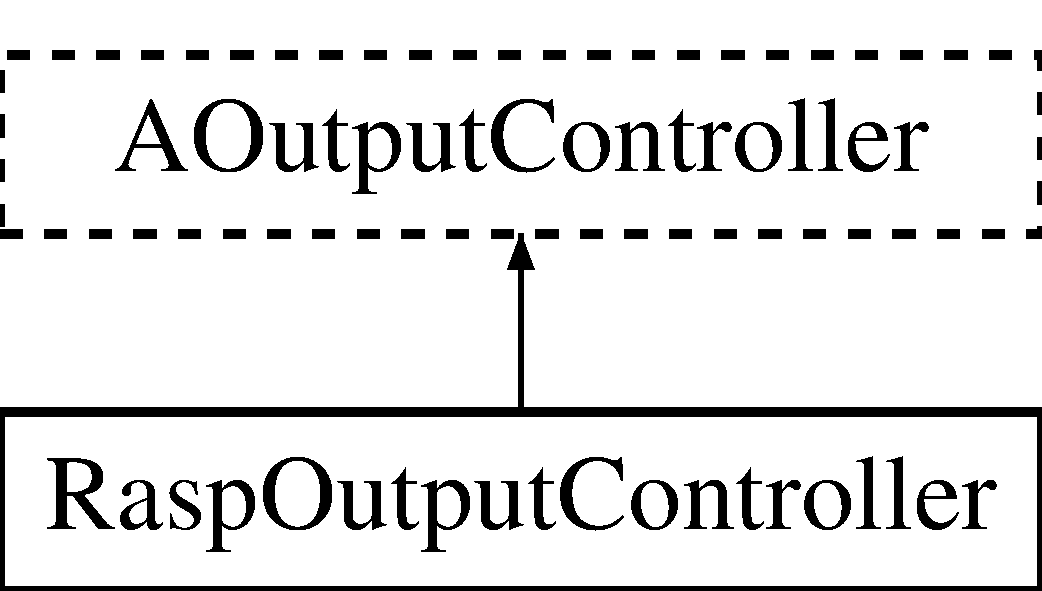
\includegraphics[height=2.000000cm]{class_rasp_output_controller}
\end{center}
\end{figure}
\subsection*{Öffentliche Methoden}
\begin{DoxyCompactItemize}
\item 
\hyperlink{class_rasp_output_controller_afd7487de7ff81c6b092f4072d4fa80a5}{Rasp\+Output\+Controller} ()
\item 
void \hyperlink{class_rasp_output_controller_afce87d510c0564567e4250b22639d5e0}{position\+Change} (unsigned short new\+Position) override
\item 
void \hyperlink{class_rasp_output_controller_a92954cf26d4dd5f7d8835d1d508302c0}{active\+Sample\+Change} (unsigned short new\+Active\+Sample, unsigned short old\+Active\+Sample) override
\item 
void \hyperlink{class_rasp_output_controller_aa084e570bcf25c75b9389ca63c875f0c}{play\+Position\+Change} (vector$<$ unsigned short $>$ \&) override
\item 
void \hyperlink{class_rasp_output_controller_a0778395ee8ec044d04fbfcb2f3b2eb04}{play\+Position\+Change} (unsigned short position, unsigned short play\+State) override
\item 
void \hyperlink{class_rasp_output_controller_a27fcbf9e1a1f9c3cefefefd537acc401}{blink} (int)
\item 
void \hyperlink{class_rasp_output_controller_a5fd551f1aba056356befd71e5bff23f1}{set\+Beat\+Duration} (unsigned int beat\+Duration) override
\item 
void \hyperlink{class_rasp_output_controller_ad195a3d664b7c7e5680cd8949203c1fc}{show\+Main\+Screen} (unsigned int bpm) override
\item 
void \hyperlink{class_rasp_output_controller_a613d3a1d1ceb31875be95e4a4b733fba}{show\+Sample\+Screen} (unsigned int bpm, float volume) override
\end{DoxyCompactItemize}
\subsection*{Private Methoden}
\begin{DoxyCompactItemize}
\item 
void \hyperlink{class_rasp_output_controller_afdd3bcfa82341a9d2539233abe7cb617}{switch\+Off\+All\+Led} ()
\item 
void \hyperlink{class_rasp_output_controller_a9a5025e13e27544721a80e6725ed23e4}{switch\+Off\+All\+Red\+Beat\+Leds} ()
\item 
void \hyperlink{class_rasp_output_controller_a1172c2966777bbcee89cbe4e6de027d5}{initialize\+Pins} ()
\item 
void \hyperlink{class_rasp_output_controller_a0cacbc3cbca8f1b78318234c6b74e576}{switch\+On\+First\+Beat\+Led} ()
\end{DoxyCompactItemize}
\subsection*{Private Attribute}
\begin{DoxyCompactItemize}
\item 
const map$<$ unsigned short, unsigned short $>$ \hyperlink{class_rasp_output_controller_afd8a9fff94ee9bcf63bcbe6fa810aa32}{output\+Pin\+Map}
\item 
const vector$<$ unsigned short $>$ \hyperlink{class_rasp_output_controller_a8ee2d3ff908d1094cc9d1320133d0bdf}{red\+Led\+List}
\item 
const vector$<$ unsigned short $>$ \hyperlink{class_rasp_output_controller_a8b888abfd8719eb95568abaf53d68d5c}{green\+Led\+List}
\item 
const vector$<$ unsigned short $>$ \hyperlink{class_rasp_output_controller_a9b5e5c4ee94d43d62e41961e6c8bea3b}{blue\+Led\+List}
\item 
const vector$<$ unsigned short $>$ \hyperlink{class_rasp_output_controller_ad0ad19b081450eb1d9cd6548c14a23ea}{sample\+Led\+List}
\item 
\hyperlink{class_display}{Display} \hyperlink{class_rasp_output_controller_a0bb52cfee18c44cd2ed64dea27d5ccc4}{display}
\item 
unsigned int \hyperlink{class_rasp_output_controller_a4deb199f7d611c2be39dc2d59ea45bba}{beat\+Blink\+Delay}
\end{DoxyCompactItemize}


\subsection{Ausführliche Beschreibung}


Definiert in Zeile 38 der Datei Rasp\+Output\+Controller.\+h.



\subsection{Beschreibung der Konstruktoren und Destruktoren}
\mbox{\Hypertarget{class_rasp_output_controller_afd7487de7ff81c6b092f4072d4fa80a5}\label{class_rasp_output_controller_afd7487de7ff81c6b092f4072d4fa80a5}} 
\index{Rasp\+Output\+Controller@{Rasp\+Output\+Controller}!Rasp\+Output\+Controller@{Rasp\+Output\+Controller}}
\index{Rasp\+Output\+Controller@{Rasp\+Output\+Controller}!Rasp\+Output\+Controller@{Rasp\+Output\+Controller}}
\subsubsection{\texorpdfstring{Rasp\+Output\+Controller()}{RaspOutputController()}}
{\footnotesize\ttfamily Rasp\+Output\+Controller\+::\+Rasp\+Output\+Controller (\begin{DoxyParamCaption}{ }\end{DoxyParamCaption})}



Definiert in Zeile 10 der Datei Rasp\+Output\+Controller.\+cpp.



Benutzt initialize\+Pins(), switch\+Off\+All\+Led() und switch\+On\+First\+Beat\+Led().



\subsection{Dokumentation der Elementfunktionen}
\mbox{\Hypertarget{class_rasp_output_controller_a92954cf26d4dd5f7d8835d1d508302c0}\label{class_rasp_output_controller_a92954cf26d4dd5f7d8835d1d508302c0}} 
\index{Rasp\+Output\+Controller@{Rasp\+Output\+Controller}!active\+Sample\+Change@{active\+Sample\+Change}}
\index{active\+Sample\+Change@{active\+Sample\+Change}!Rasp\+Output\+Controller@{Rasp\+Output\+Controller}}
\subsubsection{\texorpdfstring{active\+Sample\+Change()}{activeSampleChange()}}
{\footnotesize\ttfamily void Rasp\+Output\+Controller\+::active\+Sample\+Change (\begin{DoxyParamCaption}\item[{unsigned short}]{new\+Active\+Sample,  }\item[{unsigned short}]{old\+Active\+Sample }\end{DoxyParamCaption})\hspace{0.3cm}{\ttfamily [override]}, {\ttfamily [virtual]}}



Implementiert \hyperlink{class_a_output_controller_ac2b87aa6291c38cc65185bf6a37ae300}{A\+Output\+Controller}.



Definiert in Zeile 57 der Datei Rasp\+Output\+Controller.\+cpp.



Benutzt sample\+::\+N\+O\+\_\+\+S\+A\+M\+P\+LE, output\+Pin\+Map, switch\+Off\+All\+Red\+Beat\+Leds() und switch\+On\+First\+Beat\+Led().

\mbox{\Hypertarget{class_rasp_output_controller_a27fcbf9e1a1f9c3cefefefd537acc401}\label{class_rasp_output_controller_a27fcbf9e1a1f9c3cefefefd537acc401}} 
\index{Rasp\+Output\+Controller@{Rasp\+Output\+Controller}!blink@{blink}}
\index{blink@{blink}!Rasp\+Output\+Controller@{Rasp\+Output\+Controller}}
\subsubsection{\texorpdfstring{blink()}{blink()}}
{\footnotesize\ttfamily void Rasp\+Output\+Controller\+::blink (\begin{DoxyParamCaption}\item[{int}]{led\+Pin }\end{DoxyParamCaption})}



Definiert in Zeile 51 der Datei Rasp\+Output\+Controller.\+cpp.



Benutzt beat\+Blink\+Delay.



Wird benutzt von position\+Change() und switch\+Off\+All\+Led().

\mbox{\Hypertarget{class_rasp_output_controller_a1172c2966777bbcee89cbe4e6de027d5}\label{class_rasp_output_controller_a1172c2966777bbcee89cbe4e6de027d5}} 
\index{Rasp\+Output\+Controller@{Rasp\+Output\+Controller}!initialize\+Pins@{initialize\+Pins}}
\index{initialize\+Pins@{initialize\+Pins}!Rasp\+Output\+Controller@{Rasp\+Output\+Controller}}
\subsubsection{\texorpdfstring{initialize\+Pins()}{initializePins()}}
{\footnotesize\ttfamily void Rasp\+Output\+Controller\+::initialize\+Pins (\begin{DoxyParamCaption}{ }\end{DoxyParamCaption})\hspace{0.3cm}{\ttfamily [private]}}



Definiert in Zeile 16 der Datei Rasp\+Output\+Controller.\+cpp.



Benutzt output\+Pin\+Map.



Wird benutzt von Rasp\+Output\+Controller().

\mbox{\Hypertarget{class_rasp_output_controller_aa084e570bcf25c75b9389ca63c875f0c}\label{class_rasp_output_controller_aa084e570bcf25c75b9389ca63c875f0c}} 
\index{Rasp\+Output\+Controller@{Rasp\+Output\+Controller}!play\+Position\+Change@{play\+Position\+Change}}
\index{play\+Position\+Change@{play\+Position\+Change}!Rasp\+Output\+Controller@{Rasp\+Output\+Controller}}
\subsubsection{\texorpdfstring{play\+Position\+Change()}{playPositionChange()}\hspace{0.1cm}{\footnotesize\ttfamily [1/2]}}
{\footnotesize\ttfamily void Rasp\+Output\+Controller\+::play\+Position\+Change (\begin{DoxyParamCaption}\item[{vector$<$ unsigned short $>$ \&}]{new\+Play\+Array }\end{DoxyParamCaption})\hspace{0.3cm}{\ttfamily [override]}, {\ttfamily [virtual]}}



Implementiert \hyperlink{class_a_output_controller_a7bad658dfc3eb1223ace0c0454130818}{A\+Output\+Controller}.



Definiert in Zeile 70 der Datei Rasp\+Output\+Controller.\+cpp.

\mbox{\Hypertarget{class_rasp_output_controller_a0778395ee8ec044d04fbfcb2f3b2eb04}\label{class_rasp_output_controller_a0778395ee8ec044d04fbfcb2f3b2eb04}} 
\index{Rasp\+Output\+Controller@{Rasp\+Output\+Controller}!play\+Position\+Change@{play\+Position\+Change}}
\index{play\+Position\+Change@{play\+Position\+Change}!Rasp\+Output\+Controller@{Rasp\+Output\+Controller}}
\subsubsection{\texorpdfstring{play\+Position\+Change()}{playPositionChange()}\hspace{0.1cm}{\footnotesize\ttfamily [2/2]}}
{\footnotesize\ttfamily void Rasp\+Output\+Controller\+::play\+Position\+Change (\begin{DoxyParamCaption}\item[{unsigned short}]{position,  }\item[{unsigned short}]{play\+State }\end{DoxyParamCaption})\hspace{0.3cm}{\ttfamily [override]}, {\ttfamily [virtual]}}



Implementiert \hyperlink{class_a_output_controller_a15c1300df5606bf7d4838b41a45c31e3}{A\+Output\+Controller}.



Definiert in Zeile 77 der Datei Rasp\+Output\+Controller.\+cpp.



Benutzt state\+::\+M\+U\+TE, output\+Pin\+Map und state\+::\+P\+L\+AY.

\mbox{\Hypertarget{class_rasp_output_controller_afce87d510c0564567e4250b22639d5e0}\label{class_rasp_output_controller_afce87d510c0564567e4250b22639d5e0}} 
\index{Rasp\+Output\+Controller@{Rasp\+Output\+Controller}!position\+Change@{position\+Change}}
\index{position\+Change@{position\+Change}!Rasp\+Output\+Controller@{Rasp\+Output\+Controller}}
\subsubsection{\texorpdfstring{position\+Change()}{positionChange()}}
{\footnotesize\ttfamily void Rasp\+Output\+Controller\+::position\+Change (\begin{DoxyParamCaption}\item[{unsigned short}]{new\+Position }\end{DoxyParamCaption})\hspace{0.3cm}{\ttfamily [override]}, {\ttfamily [virtual]}}



Implementiert \hyperlink{class_a_output_controller_a5a818a40e2911411d378032b8b2fb6c8}{A\+Output\+Controller}.



Definiert in Zeile 23 der Datei Rasp\+Output\+Controller.\+cpp.



Benutzt blink() und output\+Pin\+Map.

\mbox{\Hypertarget{class_rasp_output_controller_a5fd551f1aba056356befd71e5bff23f1}\label{class_rasp_output_controller_a5fd551f1aba056356befd71e5bff23f1}} 
\index{Rasp\+Output\+Controller@{Rasp\+Output\+Controller}!set\+Beat\+Duration@{set\+Beat\+Duration}}
\index{set\+Beat\+Duration@{set\+Beat\+Duration}!Rasp\+Output\+Controller@{Rasp\+Output\+Controller}}
\subsubsection{\texorpdfstring{set\+Beat\+Duration()}{setBeatDuration()}}
{\footnotesize\ttfamily void Rasp\+Output\+Controller\+::set\+Beat\+Duration (\begin{DoxyParamCaption}\item[{unsigned int}]{beat\+Duration }\end{DoxyParamCaption})\hspace{0.3cm}{\ttfamily [override]}, {\ttfamily [virtual]}}



Implementiert \hyperlink{class_a_output_controller_ac685432fc57d2441ecb548386554d2c9}{A\+Output\+Controller}.



Definiert in Zeile 88 der Datei Rasp\+Output\+Controller.\+cpp.



Benutzt beat\+Blink\+Delay.

\mbox{\Hypertarget{class_rasp_output_controller_ad195a3d664b7c7e5680cd8949203c1fc}\label{class_rasp_output_controller_ad195a3d664b7c7e5680cd8949203c1fc}} 
\index{Rasp\+Output\+Controller@{Rasp\+Output\+Controller}!show\+Main\+Screen@{show\+Main\+Screen}}
\index{show\+Main\+Screen@{show\+Main\+Screen}!Rasp\+Output\+Controller@{Rasp\+Output\+Controller}}
\subsubsection{\texorpdfstring{show\+Main\+Screen()}{showMainScreen()}}
{\footnotesize\ttfamily void Rasp\+Output\+Controller\+::show\+Main\+Screen (\begin{DoxyParamCaption}\item[{unsigned int}]{bpm }\end{DoxyParamCaption})\hspace{0.3cm}{\ttfamily [override]}, {\ttfamily [virtual]}}



Implementiert \hyperlink{class_a_output_controller_ace7df9de71110b3615156b9bd06a9349}{A\+Output\+Controller}.



Definiert in Zeile 92 der Datei Rasp\+Output\+Controller.\+cpp.



Benutzt display und Display\+::show\+Main\+Screen().

\mbox{\Hypertarget{class_rasp_output_controller_a613d3a1d1ceb31875be95e4a4b733fba}\label{class_rasp_output_controller_a613d3a1d1ceb31875be95e4a4b733fba}} 
\index{Rasp\+Output\+Controller@{Rasp\+Output\+Controller}!show\+Sample\+Screen@{show\+Sample\+Screen}}
\index{show\+Sample\+Screen@{show\+Sample\+Screen}!Rasp\+Output\+Controller@{Rasp\+Output\+Controller}}
\subsubsection{\texorpdfstring{show\+Sample\+Screen()}{showSampleScreen()}}
{\footnotesize\ttfamily void Rasp\+Output\+Controller\+::show\+Sample\+Screen (\begin{DoxyParamCaption}\item[{unsigned int}]{bpm,  }\item[{float}]{volume }\end{DoxyParamCaption})\hspace{0.3cm}{\ttfamily [override]}, {\ttfamily [virtual]}}



Implementiert \hyperlink{class_a_output_controller_aab53d12a6aa6f38d0e4ead69e85ed4fe}{A\+Output\+Controller}.



Definiert in Zeile 96 der Datei Rasp\+Output\+Controller.\+cpp.



Benutzt display und Display\+::show\+Sample\+Screen().

\mbox{\Hypertarget{class_rasp_output_controller_afdd3bcfa82341a9d2539233abe7cb617}\label{class_rasp_output_controller_afdd3bcfa82341a9d2539233abe7cb617}} 
\index{Rasp\+Output\+Controller@{Rasp\+Output\+Controller}!switch\+Off\+All\+Led@{switch\+Off\+All\+Led}}
\index{switch\+Off\+All\+Led@{switch\+Off\+All\+Led}!Rasp\+Output\+Controller@{Rasp\+Output\+Controller}}
\subsubsection{\texorpdfstring{switch\+Off\+All\+Led()}{switchOffAllLed()}}
{\footnotesize\ttfamily void Rasp\+Output\+Controller\+::switch\+Off\+All\+Led (\begin{DoxyParamCaption}{ }\end{DoxyParamCaption})\hspace{0.3cm}{\ttfamily [private]}}



Definiert in Zeile 43 der Datei Rasp\+Output\+Controller.\+cpp.



Benutzt blink() und output\+Pin\+Map.



Wird benutzt von Rasp\+Output\+Controller().

\mbox{\Hypertarget{class_rasp_output_controller_a9a5025e13e27544721a80e6725ed23e4}\label{class_rasp_output_controller_a9a5025e13e27544721a80e6725ed23e4}} 
\index{Rasp\+Output\+Controller@{Rasp\+Output\+Controller}!switch\+Off\+All\+Red\+Beat\+Leds@{switch\+Off\+All\+Red\+Beat\+Leds}}
\index{switch\+Off\+All\+Red\+Beat\+Leds@{switch\+Off\+All\+Red\+Beat\+Leds}!Rasp\+Output\+Controller@{Rasp\+Output\+Controller}}
\subsubsection{\texorpdfstring{switch\+Off\+All\+Red\+Beat\+Leds()}{switchOffAllRedBeatLeds()}}
{\footnotesize\ttfamily void Rasp\+Output\+Controller\+::switch\+Off\+All\+Red\+Beat\+Leds (\begin{DoxyParamCaption}{ }\end{DoxyParamCaption})\hspace{0.3cm}{\ttfamily [private]}}



Definiert in Zeile 37 der Datei Rasp\+Output\+Controller.\+cpp.



Benutzt output\+Pin\+Map und red\+Led\+List.



Wird benutzt von active\+Sample\+Change().

\mbox{\Hypertarget{class_rasp_output_controller_a0cacbc3cbca8f1b78318234c6b74e576}\label{class_rasp_output_controller_a0cacbc3cbca8f1b78318234c6b74e576}} 
\index{Rasp\+Output\+Controller@{Rasp\+Output\+Controller}!switch\+On\+First\+Beat\+Led@{switch\+On\+First\+Beat\+Led}}
\index{switch\+On\+First\+Beat\+Led@{switch\+On\+First\+Beat\+Led}!Rasp\+Output\+Controller@{Rasp\+Output\+Controller}}
\subsubsection{\texorpdfstring{switch\+On\+First\+Beat\+Led()}{switchOnFirstBeatLed()}}
{\footnotesize\ttfamily void Rasp\+Output\+Controller\+::switch\+On\+First\+Beat\+Led (\begin{DoxyParamCaption}{ }\end{DoxyParamCaption})\hspace{0.3cm}{\ttfamily [private]}}



Definiert in Zeile 30 der Datei Rasp\+Output\+Controller.\+cpp.



Benutzt outputs\+::\+B\+E\+A\+T13\+\_\+\+B\+L\+UE, outputs\+::\+B\+E\+A\+T1\+\_\+\+B\+L\+UE, outputs\+::\+B\+E\+A\+T5\+\_\+\+B\+L\+UE, outputs\+::\+B\+E\+A\+T9\+\_\+\+B\+L\+UE und output\+Pin\+Map.



Wird benutzt von active\+Sample\+Change() und Rasp\+Output\+Controller().



\subsection{Dokumentation der Datenelemente}
\mbox{\Hypertarget{class_rasp_output_controller_a4deb199f7d611c2be39dc2d59ea45bba}\label{class_rasp_output_controller_a4deb199f7d611c2be39dc2d59ea45bba}} 
\index{Rasp\+Output\+Controller@{Rasp\+Output\+Controller}!beat\+Blink\+Delay@{beat\+Blink\+Delay}}
\index{beat\+Blink\+Delay@{beat\+Blink\+Delay}!Rasp\+Output\+Controller@{Rasp\+Output\+Controller}}
\subsubsection{\texorpdfstring{beat\+Blink\+Delay}{beatBlinkDelay}}
{\footnotesize\ttfamily unsigned int Rasp\+Output\+Controller\+::beat\+Blink\+Delay\hspace{0.3cm}{\ttfamily [private]}}



Definiert in Zeile 144 der Datei Rasp\+Output\+Controller.\+h.



Wird benutzt von blink() und set\+Beat\+Duration().

\mbox{\Hypertarget{class_rasp_output_controller_a9b5e5c4ee94d43d62e41961e6c8bea3b}\label{class_rasp_output_controller_a9b5e5c4ee94d43d62e41961e6c8bea3b}} 
\index{Rasp\+Output\+Controller@{Rasp\+Output\+Controller}!blue\+Led\+List@{blue\+Led\+List}}
\index{blue\+Led\+List@{blue\+Led\+List}!Rasp\+Output\+Controller@{Rasp\+Output\+Controller}}
\subsubsection{\texorpdfstring{blue\+Led\+List}{blueLedList}}
{\footnotesize\ttfamily const vector$<$unsigned short$>$ Rasp\+Output\+Controller\+::blue\+Led\+List\hspace{0.3cm}{\ttfamily [private]}}

{\bfseries Initialisierung\+:}
\begin{DoxyCode}
= \{
            \hyperlink{namespaceoutputs_a7c39d2e5116c2502c2b90bf1e8be5520}{BEAT1\_BLUE}, \hyperlink{namespaceoutputs_ac6bffee9716f79b218c8fb366351032e}{BEAT2\_BLUE}, \hyperlink{namespaceoutputs_ae87166c20e497c5b092a92bc98da94c2}{BEAT3\_BLUE}, 
      \hyperlink{namespaceoutputs_aa66f074e1960dc7dbf507acdf6cc5ae3}{BEAT4\_BLUE}, \hyperlink{namespaceoutputs_a0fab71f89a857d67f1329fbd097046ae}{BEAT5\_BLUE}, \hyperlink{namespaceoutputs_a1981eea86b118b5ff49c09ee50a75221}{BEAT6\_BLUE}, \hyperlink{namespaceoutputs_a7051f5db20e6f0c0dc7dad8775d21b1f}{BEAT7\_BLUE}, 
      \hyperlink{namespaceoutputs_a29cf0b90cc4df367e62aaaa86e7ed24e}{BEAT8\_BLUE}, \hyperlink{namespaceoutputs_a1f88716cbf83123bc10bd31b07f86b4c}{BEAT9\_BLUE},
            \hyperlink{namespaceoutputs_a188668f7db5d9610361658c817b08574}{BEAT10\_BLUE}, \hyperlink{namespaceoutputs_a31d60b8c00551d3dbeca8645eba200eb}{BEAT11\_BLUE}, \hyperlink{namespaceoutputs_ae7b144325945c1712151bf0d6a363c5f}{BEAT12\_BLUE}, 
      \hyperlink{namespaceoutputs_a38a0eba17cc5ed8eed42c37dca1feb3f}{BEAT13\_BLUE}, \hyperlink{namespaceoutputs_ab384095ae250cb117a95683710620188}{BEAT14\_BLUE}, \hyperlink{namespaceoutputs_a6d12c95904da18827ed262896b9ebaa1}{BEAT15\_BLUE}, 
      \hyperlink{namespaceoutputs_aaa4685feacdb3e8d2bb1c0435952e030}{BEAT16\_BLUE}
    \}
\end{DoxyCode}


Definiert in Zeile 129 der Datei Rasp\+Output\+Controller.\+h.

\mbox{\Hypertarget{class_rasp_output_controller_a0bb52cfee18c44cd2ed64dea27d5ccc4}\label{class_rasp_output_controller_a0bb52cfee18c44cd2ed64dea27d5ccc4}} 
\index{Rasp\+Output\+Controller@{Rasp\+Output\+Controller}!display@{display}}
\index{display@{display}!Rasp\+Output\+Controller@{Rasp\+Output\+Controller}}
\subsubsection{\texorpdfstring{display}{display}}
{\footnotesize\ttfamily \hyperlink{class_display}{Display} Rasp\+Output\+Controller\+::display\hspace{0.3cm}{\ttfamily [private]}}



Definiert in Zeile 138 der Datei Rasp\+Output\+Controller.\+h.



Wird benutzt von show\+Main\+Screen() und show\+Sample\+Screen().

\mbox{\Hypertarget{class_rasp_output_controller_a8b888abfd8719eb95568abaf53d68d5c}\label{class_rasp_output_controller_a8b888abfd8719eb95568abaf53d68d5c}} 
\index{Rasp\+Output\+Controller@{Rasp\+Output\+Controller}!green\+Led\+List@{green\+Led\+List}}
\index{green\+Led\+List@{green\+Led\+List}!Rasp\+Output\+Controller@{Rasp\+Output\+Controller}}
\subsubsection{\texorpdfstring{green\+Led\+List}{greenLedList}}
{\footnotesize\ttfamily const vector$<$unsigned short$>$ Rasp\+Output\+Controller\+::green\+Led\+List\hspace{0.3cm}{\ttfamily [private]}}

{\bfseries Initialisierung\+:}
\begin{DoxyCode}
= \{
            \hyperlink{namespaceoutputs_ad934b2db0cff1421ca84b300dc257508}{BEAT1\_GREEN}, \hyperlink{namespaceoutputs_ad2dc5e7bf8fd1c9ffa64cf8efdb0035a}{BEAT2\_GREEN}, \hyperlink{namespaceoutputs_a95e392d21973d605abcc9efc19dce314}{BEAT3\_GREEN}, 
      \hyperlink{namespaceoutputs_afd9270436632213bade739dbc4f6c8f6}{BEAT4\_GREEN}, \hyperlink{namespaceoutputs_a4b1e0d3ad2b80752a68cdec9a73f5ac6}{BEAT5\_GREEN}, \hyperlink{namespaceoutputs_a55c3bd8cf6cdffbd199abc9ae5a0e1ac}{BEAT6\_GREEN}, 
      \hyperlink{namespaceoutputs_a971ea0c6742c83be5634cbf533cfb050}{BEAT7\_GREEN}, \hyperlink{namespaceoutputs_a6fe56e04e6ce7835262e2a60df0506d6}{BEAT8\_GREEN},
            \hyperlink{namespaceoutputs_a0600b91e575643cfee3eb9e9e5b14839}{BEAT9\_GREEN}, \hyperlink{namespaceoutputs_ab0b662f329ea65f6f5fc1acba70fbd07}{BEAT10\_GREEN}, \hyperlink{namespaceoutputs_a38945c3c9766ee86e3c97a79e2be45c1}{BEAT11\_GREEN}, 
      \hyperlink{namespaceoutputs_a863de14249bb5dd32b6fb2dd665f804e}{BEAT12\_GREEN}, \hyperlink{namespaceoutputs_a3410f51b9ac465ad73e71e8bd54b3ab4}{BEAT13\_GREEN}, \hyperlink{namespaceoutputs_a181a1c13a2964de30df1c57bae8f8428}{BEAT14\_GREEN}, 
      \hyperlink{namespaceoutputs_afacd3fd74ab006d3ce548b672c3ab2f7}{BEAT15\_GREEN},
            \hyperlink{namespaceoutputs_abb8efcc194a9934c26026a359edc8929}{BEAT16\_GREEN}
    \}
\end{DoxyCode}


Definiert in Zeile 123 der Datei Rasp\+Output\+Controller.\+h.

\mbox{\Hypertarget{class_rasp_output_controller_afd8a9fff94ee9bcf63bcbe6fa810aa32}\label{class_rasp_output_controller_afd8a9fff94ee9bcf63bcbe6fa810aa32}} 
\index{Rasp\+Output\+Controller@{Rasp\+Output\+Controller}!output\+Pin\+Map@{output\+Pin\+Map}}
\index{output\+Pin\+Map@{output\+Pin\+Map}!Rasp\+Output\+Controller@{Rasp\+Output\+Controller}}
\subsubsection{\texorpdfstring{output\+Pin\+Map}{outputPinMap}}
{\footnotesize\ttfamily const map$<$unsigned short, unsigned short$>$ Rasp\+Output\+Controller\+::output\+Pin\+Map\hspace{0.3cm}{\ttfamily [private]}}



Definiert in Zeile 59 der Datei Rasp\+Output\+Controller.\+h.



Wird benutzt von active\+Sample\+Change(), initialize\+Pins(), play\+Position\+Change(), position\+Change(), switch\+Off\+All\+Led(), switch\+Off\+All\+Red\+Beat\+Leds() und switch\+On\+First\+Beat\+Led().

\mbox{\Hypertarget{class_rasp_output_controller_a8ee2d3ff908d1094cc9d1320133d0bdf}\label{class_rasp_output_controller_a8ee2d3ff908d1094cc9d1320133d0bdf}} 
\index{Rasp\+Output\+Controller@{Rasp\+Output\+Controller}!red\+Led\+List@{red\+Led\+List}}
\index{red\+Led\+List@{red\+Led\+List}!Rasp\+Output\+Controller@{Rasp\+Output\+Controller}}
\subsubsection{\texorpdfstring{red\+Led\+List}{redLedList}}
{\footnotesize\ttfamily const vector$<$unsigned short$>$ Rasp\+Output\+Controller\+::red\+Led\+List\hspace{0.3cm}{\ttfamily [private]}}

{\bfseries Initialisierung\+:}
\begin{DoxyCode}
= \{
            \hyperlink{namespaceoutputs_ae1c055268c6bbfadcc272bc6028b1a59}{BEAT1\_RED}, \hyperlink{namespaceoutputs_a7b5646e7b81bc49443f10f2b852384bb}{BEAT2\_RED}, \hyperlink{namespaceoutputs_a0c48c063f394a0735f24036e932bff2b}{BEAT3\_RED}, 
      \hyperlink{namespaceoutputs_a73a38f1135a723ebb294500daa641aec}{BEAT4\_RED}, \hyperlink{namespaceoutputs_a992a202d7fce79a524fe71498efb3709}{BEAT5\_RED}, \hyperlink{namespaceoutputs_a44e21deb20acdd11aa47bd5c2358dd6c}{BEAT6\_RED}, \hyperlink{namespaceoutputs_a88730a5804ff8785e2fb07a1957a243c}{BEAT7\_RED}, 
      \hyperlink{namespaceoutputs_aeb7e7b9874ac290d2ff579a8b144fe13}{BEAT8\_RED}, \hyperlink{namespaceoutputs_a57a4d2c831b8b263bc763032afddaa03}{BEAT9\_RED},
            \hyperlink{namespaceoutputs_a3108e2ed7adaa0c15822673c1cf5341d}{BEAT10\_RED}, \hyperlink{namespaceoutputs_a3b55bd1a681764d7655dfee327930872}{BEAT11\_RED}, \hyperlink{namespaceoutputs_a3138968cd14e309f1e88228bd1259f3f}{BEAT12\_RED}, 
      \hyperlink{namespaceoutputs_a34ead0f387c2557f9d74d57186f1578f}{BEAT13\_RED}, \hyperlink{namespaceoutputs_ae72dd425b992846bc954f41227bdda1a}{BEAT14\_RED}, \hyperlink{namespaceoutputs_a6cdbcf8d70f85316af1ea2b96d9b72bd}{BEAT15\_RED}, \hyperlink{namespaceoutputs_a3dbc6b2fd920d581b752b72f86be3733}{BEAT16\_RED}
    \}
\end{DoxyCode}


Definiert in Zeile 118 der Datei Rasp\+Output\+Controller.\+h.



Wird benutzt von switch\+Off\+All\+Red\+Beat\+Leds().

\mbox{\Hypertarget{class_rasp_output_controller_ad0ad19b081450eb1d9cd6548c14a23ea}\label{class_rasp_output_controller_ad0ad19b081450eb1d9cd6548c14a23ea}} 
\index{Rasp\+Output\+Controller@{Rasp\+Output\+Controller}!sample\+Led\+List@{sample\+Led\+List}}
\index{sample\+Led\+List@{sample\+Led\+List}!Rasp\+Output\+Controller@{Rasp\+Output\+Controller}}
\subsubsection{\texorpdfstring{sample\+Led\+List}{sampleLedList}}
{\footnotesize\ttfamily const vector$<$unsigned short$>$ Rasp\+Output\+Controller\+::sample\+Led\+List\hspace{0.3cm}{\ttfamily [private]}}

{\bfseries Initialisierung\+:}
\begin{DoxyCode}
= \{
            \hyperlink{namespaceoutputs_a151156390f60151968f4092740d9d6b8}{SAMPLE1\_LED}, \hyperlink{namespaceoutputs_ae0776935fda36be3a645994d16591980}{SAMPLE2\_LED}, \hyperlink{namespaceoutputs_a8a0be2be0ae271cb8b57234a189b6689}{SAMPLE3\_LED}, 
      \hyperlink{namespaceoutputs_a6fbee7a72f91577a7e1f072d00ad8d9f}{SAMPLE4\_LED}, \hyperlink{namespaceoutputs_a87e2d51fbeb2ac9fd23fc5d937b1c7c2}{SAMPLE5\_LED}, \hyperlink{namespaceoutputs_a7bdee2eb9fc676ac7edb9582334be15a}{SAMPLE6\_LED}, 
      \hyperlink{namespaceoutputs_a3d438bc8ce91fb825bf2da7834ac639e}{SAMPLE7\_LED}, \hyperlink{namespaceoutputs_ac6e07c06d1d512716e6309db54648440}{SAMPLE8\_LED}
    \}
\end{DoxyCode}


Definiert in Zeile 134 der Datei Rasp\+Output\+Controller.\+h.



Die Dokumentation für diese Klasse wurde erzeugt aufgrund der Dateien\+:\begin{DoxyCompactItemize}
\item 
\hyperlink{_rasp_output_controller_8h}{Rasp\+Output\+Controller.\+h}\item 
\hyperlink{_rasp_output_controller_8cpp}{Rasp\+Output\+Controller.\+cpp}\end{DoxyCompactItemize}

\hypertarget{class_sample}{}\section{Sample Klassenreferenz}
\label{class_sample}\index{Sample@{Sample}}


A class that holds and maintains information about a sample audio file, which can be played by the Drum Machine.  




{\ttfamily \#include $<$Sample.\+h$>$}

\subsection*{Öffentliche Methoden}
\begin{DoxyCompactItemize}
\item 
\hyperlink{class_sample_a7aea6b090998a430341aa6d1d6222c63}{Sample} (const char $\ast$sample\+Path)
\item 
void \hyperlink{class_sample_a5c016261d1f93a28c323a53af3ee545a}{play\+Sample} (int current\+Beat)
\item 
void \hyperlink{class_sample_a2ccc1c5571e54ba6725714cd795698f3}{play} ()
\begin{DoxyCompactList}\small\item\em Plays sample, when called. \end{DoxyCompactList}\item 
void \hyperlink{class_sample_a287eada639aedccb8908d1ae6bf67874}{play\+At\+Beat} (unsigned int beat\+Position)
\item 
void \hyperlink{class_sample_a4bf009853c35f7a29955fa2554d8e799}{toggle\+Play\+At\+Beat} (unsigned short beat\+Position)
\item 
void \hyperlink{class_sample_ae298bfb5c8c1c3c867fa962e799a2fa5}{set\+Volume} (float \hyperlink{class_sample_a74a4b4799b2bdec9fdde363992b9cec8}{volume})
\begin{DoxyCompactList}\small\item\em Setter of member volume. \end{DoxyCompactList}\item 
float \hyperlink{class_sample_a9f3c251183832a53ec1967331d022575}{get\+Volume} ()
\begin{DoxyCompactList}\small\item\em Getter of member volume. \end{DoxyCompactList}\item 
void \hyperlink{class_sample_af8ad49b65a536c535393e3968516b871}{set\+Master\+Volume} (float \hyperlink{class_sample_a74a4b4799b2bdec9fdde363992b9cec8}{volume})
\begin{DoxyCompactList}\small\item\em Setter of member master\+Volume. \end{DoxyCompactList}\item 
vector$<$ unsigned short $>$ \& \hyperlink{class_sample_a5728b28ce6f6ee19a1b84eddded4fa97}{get\+Play\+Array} ()
\end{DoxyCompactItemize}
\subsection*{Private Methoden}
\begin{DoxyCompactItemize}
\item 
void \hyperlink{class_sample_a6d13988721d2190947f65969d4737a48}{set\+Mix\+Volume} ()
\item 
float \hyperlink{class_sample_afceddb412ab50a67cb98ca6b72456f24}{get\+Master\+Volume} ()
\end{DoxyCompactItemize}
\subsection*{Private Attribute}
\begin{DoxyCompactItemize}
\item 
Mix\+\_\+\+Chunk $\ast$ \hyperlink{class_sample_ae158342c8d18a05de1c85802f7cfbd2a}{sample\+File}
\begin{DoxyCompactList}\small\item\em Pointer to. \end{DoxyCompactList}\item 
vector$<$ unsigned short $>$ \hyperlink{class_sample_a824014df7294cb94445e7ee89cc15987}{play\+Array}
\begin{DoxyCompactList}\small\item\em Vector that holds 16 zeroes or ones. One stands for an active state an zero for inactive. \end{DoxyCompactList}\item 
float \hyperlink{class_sample_a74a4b4799b2bdec9fdde363992b9cec8}{volume}
\item 
float \hyperlink{class_sample_a2d48ff8caf8425c37cf74130afb0c87a}{master\+Volume}
\end{DoxyCompactItemize}


\subsection{Ausführliche Beschreibung}
A class that holds and maintains information about a sample audio file, which can be played by the Drum Machine. 

Definiert in Zeile 32 der Datei Sample.\+h.



\subsection{Beschreibung der Konstruktoren und Destruktoren}
\mbox{\Hypertarget{class_sample_a7aea6b090998a430341aa6d1d6222c63}\label{class_sample_a7aea6b090998a430341aa6d1d6222c63}} 
\index{Sample@{Sample}!Sample@{Sample}}
\index{Sample@{Sample}!Sample@{Sample}}
\subsubsection{\texorpdfstring{Sample()}{Sample()}}
{\footnotesize\ttfamily Sample\+::\+Sample (\begin{DoxyParamCaption}\item[{const char $\ast$}]{sample\+Path }\end{DoxyParamCaption})\hspace{0.3cm}{\ttfamily [explicit]}}

Constructor 
\begin{DoxyParams}{Parameter}
{\em sample\+Path} & char\mbox{[}\mbox{]} defines where to find the audio sample file \\
\hline
\end{DoxyParams}


Definiert in Zeile 5 der Datei Sample.\+cpp.



Benutzt sample\+File.



\subsection{Dokumentation der Elementfunktionen}
\mbox{\Hypertarget{class_sample_afceddb412ab50a67cb98ca6b72456f24}\label{class_sample_afceddb412ab50a67cb98ca6b72456f24}} 
\index{Sample@{Sample}!get\+Master\+Volume@{get\+Master\+Volume}}
\index{get\+Master\+Volume@{get\+Master\+Volume}!Sample@{Sample}}
\subsubsection{\texorpdfstring{get\+Master\+Volume()}{getMasterVolume()}}
{\footnotesize\ttfamily float Sample\+::get\+Master\+Volume (\begin{DoxyParamCaption}{ }\end{DoxyParamCaption})\hspace{0.3cm}{\ttfamily [private]}}

\begin{DoxyReturn}{Rückgabe}

\end{DoxyReturn}


Definiert in Zeile 61 der Datei Sample.\+cpp.



Benutzt master\+Volume.

\mbox{\Hypertarget{class_sample_a5728b28ce6f6ee19a1b84eddded4fa97}\label{class_sample_a5728b28ce6f6ee19a1b84eddded4fa97}} 
\index{Sample@{Sample}!get\+Play\+Array@{get\+Play\+Array}}
\index{get\+Play\+Array@{get\+Play\+Array}!Sample@{Sample}}
\subsubsection{\texorpdfstring{get\+Play\+Array()}{getPlayArray()}}
{\footnotesize\ttfamily vector$<$ unsigned short, allocator$<$ unsigned short $>$ $>$ \& Sample\+::get\+Play\+Array (\begin{DoxyParamCaption}{ }\end{DoxyParamCaption})}



Definiert in Zeile 65 der Datei Sample.\+cpp.



Benutzt play\+Array.

\mbox{\Hypertarget{class_sample_a9f3c251183832a53ec1967331d022575}\label{class_sample_a9f3c251183832a53ec1967331d022575}} 
\index{Sample@{Sample}!get\+Volume@{get\+Volume}}
\index{get\+Volume@{get\+Volume}!Sample@{Sample}}
\subsubsection{\texorpdfstring{get\+Volume()}{getVolume()}}
{\footnotesize\ttfamily float Sample\+::get\+Volume (\begin{DoxyParamCaption}{ }\end{DoxyParamCaption})}



Getter of member volume. 



Definiert in Zeile 46 der Datei Sample.\+cpp.



Benutzt volume.

\mbox{\Hypertarget{class_sample_a2ccc1c5571e54ba6725714cd795698f3}\label{class_sample_a2ccc1c5571e54ba6725714cd795698f3}} 
\index{Sample@{Sample}!play@{play}}
\index{play@{play}!Sample@{Sample}}
\subsubsection{\texorpdfstring{play()}{play()}}
{\footnotesize\ttfamily void Sample\+::play (\begin{DoxyParamCaption}{ }\end{DoxyParamCaption})}



Plays sample, when called. 



Definiert in Zeile 21 der Datei Sample.\+cpp.



Benutzt sample\+File.



Wird benutzt von play\+Sample().

\mbox{\Hypertarget{class_sample_a287eada639aedccb8908d1ae6bf67874}\label{class_sample_a287eada639aedccb8908d1ae6bf67874}} 
\index{Sample@{Sample}!play\+At\+Beat@{play\+At\+Beat}}
\index{play\+At\+Beat@{play\+At\+Beat}!Sample@{Sample}}
\subsubsection{\texorpdfstring{play\+At\+Beat()}{playAtBeat()}}
{\footnotesize\ttfamily void Sample\+::play\+At\+Beat (\begin{DoxyParamCaption}\item[{unsigned int}]{beat\+Position }\end{DoxyParamCaption})}

Activates sample at the passed beat\+Position 
\begin{DoxyParams}{Parameter}
{\em beat\+Position} & the beat position, where to activate the sample \\
\hline
\end{DoxyParams}


Definiert in Zeile 31 der Datei Sample.\+cpp.



Benutzt play\+Array.



Wird benutzt von setup().

\mbox{\Hypertarget{class_sample_a5c016261d1f93a28c323a53af3ee545a}\label{class_sample_a5c016261d1f93a28c323a53af3ee545a}} 
\index{Sample@{Sample}!play\+Sample@{play\+Sample}}
\index{play\+Sample@{play\+Sample}!Sample@{Sample}}
\subsubsection{\texorpdfstring{play\+Sample()}{playSample()}}
{\footnotesize\ttfamily void Sample\+::play\+Sample (\begin{DoxyParamCaption}\item[{int}]{current\+Beat }\end{DoxyParamCaption})}

Checks if the sample is active for the passed beat position and if so, plays it 
\begin{DoxyParams}{Parameter}
{\em current\+Beat} & the current beat position of the running loop \\
\hline
\end{DoxyParams}


Definiert in Zeile 12 der Datei Sample.\+cpp.



Benutzt play() und play\+Array.

\mbox{\Hypertarget{class_sample_af8ad49b65a536c535393e3968516b871}\label{class_sample_af8ad49b65a536c535393e3968516b871}} 
\index{Sample@{Sample}!set\+Master\+Volume@{set\+Master\+Volume}}
\index{set\+Master\+Volume@{set\+Master\+Volume}!Sample@{Sample}}
\subsubsection{\texorpdfstring{set\+Master\+Volume()}{setMasterVolume()}}
{\footnotesize\ttfamily void Sample\+::set\+Master\+Volume (\begin{DoxyParamCaption}\item[{float}]{volume }\end{DoxyParamCaption})}



Setter of member master\+Volume. 



Definiert in Zeile 50 der Datei Sample.\+cpp.



Benutzt master\+Volume, set\+Mix\+Volume() und volume.



Wird benutzt von Drum\+Machine\+::add\+Sample().

\mbox{\Hypertarget{class_sample_a6d13988721d2190947f65969d4737a48}\label{class_sample_a6d13988721d2190947f65969d4737a48}} 
\index{Sample@{Sample}!set\+Mix\+Volume@{set\+Mix\+Volume}}
\index{set\+Mix\+Volume@{set\+Mix\+Volume}!Sample@{Sample}}
\subsubsection{\texorpdfstring{set\+Mix\+Volume()}{setMixVolume()}}
{\footnotesize\ttfamily void Sample\+::set\+Mix\+Volume (\begin{DoxyParamCaption}{ }\end{DoxyParamCaption})\hspace{0.3cm}{\ttfamily [private]}}



Definiert in Zeile 25 der Datei Sample.\+cpp.



Benutzt master\+Volume, sample\+File und volume.



Wird benutzt von set\+Master\+Volume() und set\+Volume().

\mbox{\Hypertarget{class_sample_ae298bfb5c8c1c3c867fa962e799a2fa5}\label{class_sample_ae298bfb5c8c1c3c867fa962e799a2fa5}} 
\index{Sample@{Sample}!set\+Volume@{set\+Volume}}
\index{set\+Volume@{set\+Volume}!Sample@{Sample}}
\subsubsection{\texorpdfstring{set\+Volume()}{setVolume()}}
{\footnotesize\ttfamily void Sample\+::set\+Volume (\begin{DoxyParamCaption}\item[{float}]{volume }\end{DoxyParamCaption})}



Setter of member volume. 



Definiert in Zeile 35 der Datei Sample.\+cpp.



Benutzt set\+Mix\+Volume() und volume.

\mbox{\Hypertarget{class_sample_a4bf009853c35f7a29955fa2554d8e799}\label{class_sample_a4bf009853c35f7a29955fa2554d8e799}} 
\index{Sample@{Sample}!toggle\+Play\+At\+Beat@{toggle\+Play\+At\+Beat}}
\index{toggle\+Play\+At\+Beat@{toggle\+Play\+At\+Beat}!Sample@{Sample}}
\subsubsection{\texorpdfstring{toggle\+Play\+At\+Beat()}{togglePlayAtBeat()}}
{\footnotesize\ttfamily void Sample\+::toggle\+Play\+At\+Beat (\begin{DoxyParamCaption}\item[{unsigned short}]{beat\+Position }\end{DoxyParamCaption})}

Toggles sample state at the passed beat\+Position from active to inactive or vice versa 
\begin{DoxyParams}{Parameter}
{\em beat\+Position} & the beat position where to toggle the sample state \\
\hline
\end{DoxyParams}


Definiert in Zeile 69 der Datei Sample.\+cpp.



Benutzt state\+::\+M\+U\+TE, state\+::\+P\+L\+AY und play\+Array.



\subsection{Dokumentation der Datenelemente}
\mbox{\Hypertarget{class_sample_a2d48ff8caf8425c37cf74130afb0c87a}\label{class_sample_a2d48ff8caf8425c37cf74130afb0c87a}} 
\index{Sample@{Sample}!master\+Volume@{master\+Volume}}
\index{master\+Volume@{master\+Volume}!Sample@{Sample}}
\subsubsection{\texorpdfstring{master\+Volume}{masterVolume}}
{\footnotesize\ttfamily float Sample\+::master\+Volume\hspace{0.3cm}{\ttfamily [private]}}



Definiert in Zeile 80 der Datei Sample.\+h.



Wird benutzt von get\+Master\+Volume(), set\+Master\+Volume() und set\+Mix\+Volume().

\mbox{\Hypertarget{class_sample_a824014df7294cb94445e7ee89cc15987}\label{class_sample_a824014df7294cb94445e7ee89cc15987}} 
\index{Sample@{Sample}!play\+Array@{play\+Array}}
\index{play\+Array@{play\+Array}!Sample@{Sample}}
\subsubsection{\texorpdfstring{play\+Array}{playArray}}
{\footnotesize\ttfamily vector$<$unsigned short$>$ Sample\+::play\+Array\hspace{0.3cm}{\ttfamily [private]}}



Vector that holds 16 zeroes or ones. One stands for an active state an zero for inactive. 



Definiert in Zeile 78 der Datei Sample.\+h.



Wird benutzt von get\+Play\+Array(), play\+At\+Beat(), play\+Sample() und toggle\+Play\+At\+Beat().

\mbox{\Hypertarget{class_sample_ae158342c8d18a05de1c85802f7cfbd2a}\label{class_sample_ae158342c8d18a05de1c85802f7cfbd2a}} 
\index{Sample@{Sample}!sample\+File@{sample\+File}}
\index{sample\+File@{sample\+File}!Sample@{Sample}}
\subsubsection{\texorpdfstring{sample\+File}{sampleFile}}
{\footnotesize\ttfamily Mix\+\_\+\+Chunk$\ast$ Sample\+::sample\+File\hspace{0.3cm}{\ttfamily [private]}}



Pointer to. 



Definiert in Zeile 77 der Datei Sample.\+h.



Wird benutzt von play(), Sample() und set\+Mix\+Volume().

\mbox{\Hypertarget{class_sample_a74a4b4799b2bdec9fdde363992b9cec8}\label{class_sample_a74a4b4799b2bdec9fdde363992b9cec8}} 
\index{Sample@{Sample}!volume@{volume}}
\index{volume@{volume}!Sample@{Sample}}
\subsubsection{\texorpdfstring{volume}{volume}}
{\footnotesize\ttfamily float Sample\+::volume\hspace{0.3cm}{\ttfamily [private]}}



Definiert in Zeile 79 der Datei Sample.\+h.



Wird benutzt von get\+Volume(), set\+Master\+Volume(), set\+Mix\+Volume() und set\+Volume().



Die Dokumentation für diese Klasse wurde erzeugt aufgrund der Dateien\+:\begin{DoxyCompactItemize}
\item 
\hyperlink{_sample_8h}{Sample.\+h}\item 
\hyperlink{_sample_8cpp}{Sample.\+cpp}\end{DoxyCompactItemize}

\hypertarget{class_timer}{}\section{Timer Class Reference}
\label{class_timer}\index{Timer@{Timer}}


Call a callback function in a given interval, determining the time with a given precision. Higher precision means higher demand in resources.  




{\ttfamily \#include $<$Timer.\+h$>$}

\subsection*{Public Member Functions}
\begin{DoxyCompactItemize}
\item 
\hyperlink{class_timer_a5b659c4fb572c549dad183a7b32b08df}{Timer} (unsigned int \hyperlink{class_timer_aaf9bce1286b714658a0f4484d8fee960}{interval}, unsigned int \hyperlink{class_timer_a3d1026dd88596a97cb6b768f475ed57f}{precision})
\item 
{\footnotesize template$<$typename Function , typename... Args$>$ }\\void \hyperlink{class_timer_adcf70b5065e31461e27309c96065437a}{start} (Function \&\&callback, Args \&\&... args)
\item 
void \hyperlink{class_timer_a63f0eb44b27402196590a03781515dba}{stop} ()
\item 
unsigned int \hyperlink{class_timer_a6cbb88b5073d95fd871a012966005618}{get\+Interval} () const
\item 
void \hyperlink{class_timer_a0b24293bfc154f7432b1c52ac857d853}{set\+Interval} (unsigned int \hyperlink{class_timer_aaf9bce1286b714658a0f4484d8fee960}{interval})
\end{DoxyCompactItemize}
\subsection*{Private Member Functions}
\begin{DoxyCompactItemize}
\item 
long long \hyperlink{class_timer_a39a332f8ce3a45ed8d78c772755342c8}{get\+Current\+Time\+Millis} ()
\end{DoxyCompactItemize}
\subsection*{Private Attributes}
\begin{DoxyCompactItemize}
\item 
unsigned int \hyperlink{class_timer_a3d1026dd88596a97cb6b768f475ed57f}{precision}
\begin{DoxyCompactList}\small\item\em The precision in nanoseconds. \end{DoxyCompactList}\item 
unsigned int \hyperlink{class_timer_aaf9bce1286b714658a0f4484d8fee960}{interval}
\begin{DoxyCompactList}\small\item\em The interval in milliseconds. \end{DoxyCompactList}\item 
bool \hyperlink{class_timer_a3b8bb57a0a252c88f85c0592715ea425}{running}
\begin{DoxyCompactList}\small\item\em Is the timer currently running. \end{DoxyCompactList}\end{DoxyCompactItemize}


\subsection{Detailed Description}
Call a callback function in a given interval, determining the time with a given precision. Higher precision means higher demand in resources. 

Definition at line 17 of file Timer.\+h.



\subsection{Constructor \& Destructor Documentation}
\mbox{\Hypertarget{class_timer_a5b659c4fb572c549dad183a7b32b08df}\label{class_timer_a5b659c4fb572c549dad183a7b32b08df}} 
\index{Timer@{Timer}!Timer@{Timer}}
\index{Timer@{Timer}!Timer@{Timer}}
\subsubsection{\texorpdfstring{Timer()}{Timer()}}
{\footnotesize\ttfamily Timer\+::\+Timer (\begin{DoxyParamCaption}\item[{unsigned int}]{interval,  }\item[{unsigned int}]{precision }\end{DoxyParamCaption})}

Constructor 
\begin{DoxyParams}{Parameters}
{\em interval} & the interval in milliseconds in which the callback function is called. \\
\hline
{\em precision} & the precision in nanoseconds with which to determine the current time. Higher precision means higher demand in resources. \\
\hline
\end{DoxyParams}


Definition at line 5 of file Timer.\+cpp.



\subsection{Member Function Documentation}
\mbox{\Hypertarget{class_timer_a39a332f8ce3a45ed8d78c772755342c8}\label{class_timer_a39a332f8ce3a45ed8d78c772755342c8}} 
\index{Timer@{Timer}!get\+Current\+Time\+Millis@{get\+Current\+Time\+Millis}}
\index{get\+Current\+Time\+Millis@{get\+Current\+Time\+Millis}!Timer@{Timer}}
\subsubsection{\texorpdfstring{get\+Current\+Time\+Millis()}{getCurrentTimeMillis()}}
{\footnotesize\ttfamily long long Timer\+::get\+Current\+Time\+Millis (\begin{DoxyParamCaption}{ }\end{DoxyParamCaption})\hspace{0.3cm}{\ttfamily [inline]}, {\ttfamily [private]}}

$<$ Helper function to get the current time in milliseconds 

Definition at line 23 of file Timer.\+h.

\mbox{\Hypertarget{class_timer_a6cbb88b5073d95fd871a012966005618}\label{class_timer_a6cbb88b5073d95fd871a012966005618}} 
\index{Timer@{Timer}!get\+Interval@{get\+Interval}}
\index{get\+Interval@{get\+Interval}!Timer@{Timer}}
\subsubsection{\texorpdfstring{get\+Interval()}{getInterval()}}
{\footnotesize\ttfamily unsigned int Timer\+::get\+Interval (\begin{DoxyParamCaption}{ }\end{DoxyParamCaption}) const}

\begin{DoxyReturn}{Returns}
the interval with which the timer calls the callback function. 
\end{DoxyReturn}


Definition at line 11 of file Timer.\+cpp.



References interval.

\mbox{\Hypertarget{class_timer_a0b24293bfc154f7432b1c52ac857d853}\label{class_timer_a0b24293bfc154f7432b1c52ac857d853}} 
\index{Timer@{Timer}!set\+Interval@{set\+Interval}}
\index{set\+Interval@{set\+Interval}!Timer@{Timer}}
\subsubsection{\texorpdfstring{set\+Interval()}{setInterval()}}
{\footnotesize\ttfamily void Timer\+::set\+Interval (\begin{DoxyParamCaption}\item[{unsigned int}]{interval }\end{DoxyParamCaption})}


\begin{DoxyParams}{Parameters}
{\em interval} & the interval with which the timer calls the callback function. \\
\hline
\end{DoxyParams}


Definition at line 15 of file Timer.\+cpp.



References interval.



Referenced by Drum\+Machine\+::set\+B\+P\+M(), and Drum\+Machine\+::start\+Loop().

\mbox{\Hypertarget{class_timer_adcf70b5065e31461e27309c96065437a}\label{class_timer_adcf70b5065e31461e27309c96065437a}} 
\index{Timer@{Timer}!start@{start}}
\index{start@{start}!Timer@{Timer}}
\subsubsection{\texorpdfstring{start()}{start()}}
{\footnotesize\ttfamily template$<$typename Function , typename... Args$>$ \\
void Timer\+::start (\begin{DoxyParamCaption}\item[{Function \&\&}]{callback,  }\item[{Args \&\&...}]{args }\end{DoxyParamCaption})\hspace{0.3cm}{\ttfamily [inline]}}

Starts the timer. 
\begin{DoxyParams}{Parameters}
{\em callback} & the callback function the timer calls in the determined interval. \\
\hline
{\em args} & arguments to pass to the callback function upon call. \\
\hline
\end{DoxyParams}


Definition at line 42 of file Timer.\+h.



Referenced by Drum\+Machine\+::start\+Loop(), and Rasp\+Input\+Controller\+::start\+Polling().

\mbox{\Hypertarget{class_timer_a63f0eb44b27402196590a03781515dba}\label{class_timer_a63f0eb44b27402196590a03781515dba}} 
\index{Timer@{Timer}!stop@{stop}}
\index{stop@{stop}!Timer@{Timer}}
\subsubsection{\texorpdfstring{stop()}{stop()}}
{\footnotesize\ttfamily void Timer\+::stop (\begin{DoxyParamCaption}{ }\end{DoxyParamCaption})}

Stops the timer 

Definition at line 7 of file Timer.\+cpp.



References running.



Referenced by Rasp\+Input\+Controller\+::stop(), and Drum\+Machine\+::stop\+Loop().



\subsection{Member Data Documentation}
\mbox{\Hypertarget{class_timer_aaf9bce1286b714658a0f4484d8fee960}\label{class_timer_aaf9bce1286b714658a0f4484d8fee960}} 
\index{Timer@{Timer}!interval@{interval}}
\index{interval@{interval}!Timer@{Timer}}
\subsubsection{\texorpdfstring{interval}{interval}}
{\footnotesize\ttfamily unsigned int Timer\+::interval\hspace{0.3cm}{\ttfamily [private]}}



The interval in milliseconds. 



Definition at line 20 of file Timer.\+h.



Referenced by get\+Interval(), and set\+Interval().

\mbox{\Hypertarget{class_timer_a3d1026dd88596a97cb6b768f475ed57f}\label{class_timer_a3d1026dd88596a97cb6b768f475ed57f}} 
\index{Timer@{Timer}!precision@{precision}}
\index{precision@{precision}!Timer@{Timer}}
\subsubsection{\texorpdfstring{precision}{precision}}
{\footnotesize\ttfamily unsigned int Timer\+::precision\hspace{0.3cm}{\ttfamily [private]}}



The precision in nanoseconds. 



Definition at line 19 of file Timer.\+h.

\mbox{\Hypertarget{class_timer_a3b8bb57a0a252c88f85c0592715ea425}\label{class_timer_a3b8bb57a0a252c88f85c0592715ea425}} 
\index{Timer@{Timer}!running@{running}}
\index{running@{running}!Timer@{Timer}}
\subsubsection{\texorpdfstring{running}{running}}
{\footnotesize\ttfamily bool Timer\+::running\hspace{0.3cm}{\ttfamily [private]}}



Is the timer currently running. 



Definition at line 21 of file Timer.\+h.



Referenced by stop().



The documentation for this class was generated from the following files\+:\begin{DoxyCompactItemize}
\item 
\hyperlink{_timer_8h}{Timer.\+h}\item 
\hyperlink{_timer_8cpp}{Timer.\+cpp}\end{DoxyCompactItemize}

\chapter{File Documentation}
\hypertarget{_a_output_controller_8h}{}\section{A\+Output\+Controller.\+h-\/\+Dateireferenz}
\label{_a_output_controller_8h}\index{A\+Output\+Controller.\+h@{A\+Output\+Controller.\+h}}
{\ttfamily \#include $<$vector$>$}\newline
\subsection*{Klassen}
\begin{DoxyCompactItemize}
\item 
class \hyperlink{class_a_output_controller}{A\+Output\+Controller}
\end{DoxyCompactItemize}

\hypertarget{_display_8cpp}{}\section{Display.\+cpp File Reference}
\label{_display_8cpp}\index{Display.\+cpp@{Display.\+cpp}}
{\ttfamily \#include \char`\"{}Display.\+h\char`\"{}}\newline

\hypertarget{_display_8h}{}\section{Display.\+h-\/\+Dateireferenz}
\label{_display_8h}\index{Display.\+h@{Display.\+h}}
{\ttfamily \#include $<$Ardui\+Pi\+\_\+\+S\+S\+D1306.\+h$>$}\newline
{\ttfamily \#include $<$Adafruit\+\_\+\+G\+F\+X.\+h$>$}\newline
{\ttfamily \#include $<$Adafruit\+\_\+\+S\+S\+D1306.\+h$>$}\newline
\subsection*{Klassen}
\begin{DoxyCompactItemize}
\item 
class \hyperlink{class_display}{Display}
\end{DoxyCompactItemize}

\hypertarget{_drum_machine_8cpp}{}\section{Drum\+Machine.\+cpp File Reference}
\label{_drum_machine_8cpp}\index{Drum\+Machine.\+cpp@{Drum\+Machine.\+cpp}}
{\ttfamily \#include $<$S\+D\+L2/\+S\+D\+L.\+h$>$}\newline
{\ttfamily \#include $<$chrono$>$}\newline
{\ttfamily \#include $<$iostream$>$}\newline
{\ttfamily \#include \char`\"{}Drum\+Machine.\+h\char`\"{}}\newline

\hypertarget{_drum_machine_8h}{}\section{Drum\+Machine.\+h-\/\+Dateireferenz}
\label{_drum_machine_8h}\index{Drum\+Machine.\+h@{Drum\+Machine.\+h}}
{\ttfamily \#include $<$vector$>$}\newline
{\ttfamily \#include \char`\"{}Sample.\+h\char`\"{}}\newline
{\ttfamily \#include \char`\"{}A\+Output\+Controller.\+h\char`\"{}}\newline
{\ttfamily \#include \char`\"{}Rasp\+Output\+Controller.\+h\char`\"{}}\newline
{\ttfamily \#include \char`\"{}Timer.\+h\char`\"{}}\newline
\subsection*{Klassen}
\begin{DoxyCompactItemize}
\item 
class \hyperlink{class_drum_machine}{Drum\+Machine}
\begin{DoxyCompactList}\small\item\em Handles the beat loop and samples including correct timing for the give B\+PM, playing them at the correct beat steps and increasing and decreasing the volume. \end{DoxyCompactList}\end{DoxyCompactItemize}
\subsection*{Namensbereiche}
\begin{DoxyCompactItemize}
\item 
 \hyperlink{namespacesample}{sample}
\item 
 \hyperlink{namespacebeat}{beat}
\end{DoxyCompactItemize}
\subsection*{Variablen}
\begin{DoxyCompactItemize}
\item 
const unsigned short \hyperlink{namespacesample_a59478bc0929eb3127ff4ed573d5abab5}{sample\+::\+S\+A\+M\+P\+L\+E1} = 0
\item 
const unsigned short \hyperlink{namespacesample_a74decdde1db22f406d0a0cc1857534f4}{sample\+::\+S\+A\+M\+P\+L\+E2} = 1
\item 
const unsigned short \hyperlink{namespacesample_ac0aab16a33bfcdbd978ad2efd28cd85a}{sample\+::\+S\+A\+M\+P\+L\+E3} = 2
\item 
const unsigned short \hyperlink{namespacesample_ac15354120ebb7dccc9ba3f548e996148}{sample\+::\+S\+A\+M\+P\+L\+E4} = 3
\item 
const unsigned short \hyperlink{namespacesample_ae4dc2e0aefa868bda5be2fcdc695ef4e}{sample\+::\+S\+A\+M\+P\+L\+E5} = 4
\item 
const unsigned short \hyperlink{namespacesample_af6cf4e0873f330ffdf8d341aca16d6cc}{sample\+::\+S\+A\+M\+P\+L\+E6} = 5
\item 
const unsigned short \hyperlink{namespacesample_ad35669bc942fa6aa53d1d261f7257a3e}{sample\+::\+S\+A\+M\+P\+L\+E7} = 6
\item 
const unsigned short \hyperlink{namespacesample_a941e99fc5405e8c43f53d75c486d0819}{sample\+::\+S\+A\+M\+P\+L\+E8} = 7
\item 
const unsigned short \hyperlink{namespacesample_aa6106026bc40989292431c65c348a659}{sample\+::\+N\+O\+\_\+\+S\+A\+M\+P\+LE} = 8
\item 
const unsigned short \hyperlink{namespacebeat_ae859561033de8f2140542a8bea7d5f02}{beat\+::\+B\+E\+A\+T1} = 0
\item 
const unsigned short \hyperlink{namespacebeat_a219eb8f5f0218df3af3f4d4d9214327f}{beat\+::\+B\+E\+A\+T2} = 1
\item 
const unsigned short \hyperlink{namespacebeat_a0ccf0d5bdc6dfdae1fd7b1667655a18f}{beat\+::\+B\+E\+A\+T3} = 2
\item 
const unsigned short \hyperlink{namespacebeat_acb66407079f4f750c8edf7c1bd8519df}{beat\+::\+B\+E\+A\+T4} = 3
\item 
const unsigned short \hyperlink{namespacebeat_a1707525607992183af84b75b13bdcf1c}{beat\+::\+B\+E\+A\+T5} = 4
\item 
const unsigned short \hyperlink{namespacebeat_a38be39fd5d7424553131d77620a5fbfc}{beat\+::\+B\+E\+A\+T6} = 5
\item 
const unsigned short \hyperlink{namespacebeat_af4ce75f48a22e0f3aacded8385030cad}{beat\+::\+B\+E\+A\+T7} = 6
\item 
const unsigned short \hyperlink{namespacebeat_a564212b647573e2f3fce876049227d2c}{beat\+::\+B\+E\+A\+T8} = 7
\item 
const unsigned short \hyperlink{namespacebeat_a6558138490436cdf9a77d90ffd07e092}{beat\+::\+B\+E\+A\+T9} = 8
\item 
const unsigned short \hyperlink{namespacebeat_abd0eb0f3160a3579b574ffa8bf94282c}{beat\+::\+B\+E\+A\+T10} = 9
\item 
const unsigned short \hyperlink{namespacebeat_a4ba76b47d18db4674af1ca28136614e2}{beat\+::\+B\+E\+A\+T11} = 10
\item 
const unsigned short \hyperlink{namespacebeat_ae84780c2b37cac562b4f9e7676d7a715}{beat\+::\+B\+E\+A\+T12} = 11
\item 
const unsigned short \hyperlink{namespacebeat_a0056cac49aa9cd40c0532068b40322fe}{beat\+::\+B\+E\+A\+T13} = 12
\item 
const unsigned short \hyperlink{namespacebeat_aa25c9d3e796af023ea86fc1181ff4732}{beat\+::\+B\+E\+A\+T14} = 13
\item 
const unsigned short \hyperlink{namespacebeat_a241a13409659dff75e5368358447fc73}{beat\+::\+B\+E\+A\+T15} = 14
\item 
const unsigned short \hyperlink{namespacebeat_ad619f02c1a78c30570d7371411f1ef47}{beat\+::\+B\+E\+A\+T16} = 15
\end{DoxyCompactItemize}

\hypertarget{_drum_machine_input_listener_8cpp}{}\section{Drum\+Machine\+Input\+Listener.\+cpp-\/\+Dateireferenz}
\label{_drum_machine_input_listener_8cpp}\index{Drum\+Machine\+Input\+Listener.\+cpp@{Drum\+Machine\+Input\+Listener.\+cpp}}
{\ttfamily \#include \char`\"{}Drum\+Machine\+Input\+Listener.\+h\char`\"{}}\newline
{\ttfamily \#include \char`\"{}Rasp\+Input\+Controller.\+h\char`\"{}}\newline

\hypertarget{_drum_machine_input_listener_8h}{}\section{Drum\+Machine\+Input\+Listener.\+h-\/\+Dateireferenz}
\label{_drum_machine_input_listener_8h}\index{Drum\+Machine\+Input\+Listener.\+h@{Drum\+Machine\+Input\+Listener.\+h}}
{\ttfamily \#include \char`\"{}Drum\+Machine.\+h\char`\"{}}\newline
{\ttfamily \#include \char`\"{}Input\+Listener.\+h\char`\"{}}\newline
\subsection*{Klassen}
\begin{DoxyCompactItemize}
\item 
class \hyperlink{class_drum_machine_input_listener}{Drum\+Machine\+Input\+Listener}
\begin{DoxyCompactList}\small\item\em \hyperlink{class_input_listener}{Input\+Listener} implementation for the drum machine to handle input events. \end{DoxyCompactList}\end{DoxyCompactItemize}

\hypertarget{_input_listener_8h}{}\section{Input\+Listener.\+h File Reference}
\label{_input_listener_8h}\index{Input\+Listener.\+h@{Input\+Listener.\+h}}
{\ttfamily \#include $<$vector$>$}\newline
\subsection*{Classes}
\begin{DoxyCompactItemize}
\item 
class \hyperlink{class_input_listener}{Input\+Listener}
\begin{DoxyCompactList}\small\item\em Interface for input listeners to register in the \hyperlink{class_rasp_input_controller}{Rasp\+Input\+Controller}. \end{DoxyCompactList}\end{DoxyCompactItemize}

\hypertarget{main_8cpp}{}\section{main.\+cpp File Reference}
\label{main_8cpp}\index{main.\+cpp@{main.\+cpp}}
{\ttfamily \#include $<$mcp23017.\+h$>$}\newline
{\ttfamily \#include $<$wiring\+Pi.\+h$>$}\newline
{\ttfamily \#include \char`\"{}Drum\+Machine.\+h\char`\"{}}\newline
{\ttfamily \#include \char`\"{}Input\+Listener.\+h\char`\"{}}\newline
{\ttfamily \#include \char`\"{}Rasp\+Input\+Controller.\+h\char`\"{}}\newline
{\ttfamily \#include \char`\"{}Drum\+Machine\+Input\+Listener.\+h\char`\"{}}\newline
\subsection*{Functions}
\begin{DoxyCompactItemize}
\item 
void \hyperlink{main_8cpp_a73e5135dcf1892c3d2ff55a7b486e7d2}{setup} (\hyperlink{class_drum_machine}{Drum\+Machine} \&drum\+Machine)
\item 
int \hyperlink{main_8cpp_ae66f6b31b5ad750f1fe042a706a4e3d4}{main} ()
\end{DoxyCompactItemize}


\subsection{Function Documentation}
\mbox{\Hypertarget{main_8cpp_ae66f6b31b5ad750f1fe042a706a4e3d4}\label{main_8cpp_ae66f6b31b5ad750f1fe042a706a4e3d4}} 
\index{main.\+cpp@{main.\+cpp}!main@{main}}
\index{main@{main}!main.\+cpp@{main.\+cpp}}
\subsubsection{\texorpdfstring{main()}{main()}}
{\footnotesize\ttfamily int main (\begin{DoxyParamCaption}{ }\end{DoxyParamCaption})}



Definition at line 43 of file main.\+cpp.



References Rasp\+Input\+Controller\+::add\+Input\+Listener(), setup(), and Rasp\+Input\+Controller\+::start().

\mbox{\Hypertarget{main_8cpp_a73e5135dcf1892c3d2ff55a7b486e7d2}\label{main_8cpp_a73e5135dcf1892c3d2ff55a7b486e7d2}} 
\index{main.\+cpp@{main.\+cpp}!setup@{setup}}
\index{setup@{setup}!main.\+cpp@{main.\+cpp}}
\subsubsection{\texorpdfstring{setup()}{setup()}}
{\footnotesize\ttfamily void setup (\begin{DoxyParamCaption}\item[{\hyperlink{class_drum_machine}{Drum\+Machine} \&}]{drum\+Machine }\end{DoxyParamCaption})}



Definition at line 11 of file main.\+cpp.



References Drum\+Machine\+::add\+Sample(), Sample\+::play\+At\+Beat(), and Drum\+Machine\+::set\+B\+P\+M().



Referenced by main().


\hypertarget{_rasp_input_controller_8cpp}{}\section{Rasp\+Input\+Controller.\+cpp File Reference}
\label{_rasp_input_controller_8cpp}\index{Rasp\+Input\+Controller.\+cpp@{Rasp\+Input\+Controller.\+cpp}}
{\ttfamily \#include $<$wiring\+Pi.\+h$>$}\newline
{\ttfamily \#include \char`\"{}Rasp\+Input\+Controller.\+h\char`\"{}}\newline

\hypertarget{_rasp_input_controller_8h}{}\section{Rasp\+Input\+Controller.\+h-\/\+Dateireferenz}
\label{_rasp_input_controller_8h}\index{Rasp\+Input\+Controller.\+h@{Rasp\+Input\+Controller.\+h}}
{\ttfamily \#include \char`\"{}Drum\+Machine.\+h\char`\"{}}\newline
{\ttfamily \#include \char`\"{}Input\+Listener.\+h\char`\"{}}\newline
{\ttfamily \#include $<$wiring\+Pi.\+h$>$}\newline
\subsection*{Klassen}
\begin{DoxyCompactItemize}
\item 
class \hyperlink{class_rasp_input_controller}{Rasp\+Input\+Controller}
\end{DoxyCompactItemize}
\subsection*{Namensbereiche}
\begin{DoxyCompactItemize}
\item 
 \hyperlink{namespaceinputs}{inputs}
\end{DoxyCompactItemize}
\subsection*{Variablen}
\begin{DoxyCompactItemize}
\item 
const unsigned short \hyperlink{namespaceinputs_ab1d58fe937ccabff6ec4011a74028bfb}{inputs\+::\+V\+O\+L\+U\+M\+E\+\_\+\+B\+P\+M\+\_\+\+U\+P\+\_\+\+B\+U\+T\+T\+ON} = 1
\item 
const unsigned short \hyperlink{namespaceinputs_af3cad6ab00b2670e1710698945d28c17}{inputs\+::\+V\+O\+L\+U\+M\+E\+\_\+\+B\+P\+M\+\_\+\+D\+O\+W\+N\+\_\+\+B\+U\+T\+T\+ON} = 2
\item 
const unsigned short \hyperlink{namespaceinputs_af0075a72395787966efcec2403306b43}{inputs\+::\+M\+U\+T\+E\+\_\+\+B\+U\+T\+T\+ON} = 5
\item 
const unsigned short \hyperlink{namespaceinputs_a39dbaf6935309e198c1a0bc6e3468c45}{inputs\+::\+S\+A\+M\+P\+L\+E1\+\_\+\+B\+U\+T\+T\+ON} = 6
\item 
const unsigned short \hyperlink{namespaceinputs_afcf2086c7f58f801e5654d8e573d928c}{inputs\+::\+S\+A\+M\+P\+L\+E2\+\_\+\+B\+U\+T\+T\+ON} = 7
\item 
const unsigned short \hyperlink{namespaceinputs_a17158d35ca30fb91c6f9f757ce0d7ccc}{inputs\+::\+S\+A\+M\+P\+L\+E3\+\_\+\+B\+U\+T\+T\+ON} = 8
\item 
const unsigned short \hyperlink{namespaceinputs_ac9ccac580f0955e454a367ddc6421d78}{inputs\+::\+S\+A\+M\+P\+L\+E4\+\_\+\+B\+U\+T\+T\+ON} = 9
\item 
const unsigned short \hyperlink{namespaceinputs_ad22ade847b4a38fd418dccda07814551}{inputs\+::\+S\+A\+M\+P\+L\+E5\+\_\+\+B\+U\+T\+T\+ON} = 10
\item 
const unsigned short \hyperlink{namespaceinputs_a88edcfa8b89df1abcca33bcec05974c4}{inputs\+::\+S\+A\+M\+P\+L\+E6\+\_\+\+B\+U\+T\+T\+ON} = 11
\item 
const unsigned short \hyperlink{namespaceinputs_a50972dcf524a7b7c420ca75b0ba72a29}{inputs\+::\+S\+A\+M\+P\+L\+E7\+\_\+\+B\+U\+T\+T\+ON} = 12
\item 
const unsigned short \hyperlink{namespaceinputs_a85f389284c616cd584390d04ad192ced}{inputs\+::\+S\+A\+M\+P\+L\+E8\+\_\+\+B\+U\+T\+T\+ON} = 13
\item 
const unsigned short \hyperlink{namespaceinputs_af62021422f469c370f42c78a72504a66}{inputs\+::\+B\+E\+A\+T1\+\_\+\+B\+U\+T\+T\+ON} = 14
\item 
const unsigned short \hyperlink{namespaceinputs_a8cdd33c9e53b617a2cf8bd32a5b74484}{inputs\+::\+B\+E\+A\+T2\+\_\+\+B\+U\+T\+T\+ON} = 15
\item 
const unsigned short \hyperlink{namespaceinputs_ab60a6fc2188a034f76d3fbe554efe314}{inputs\+::\+B\+E\+A\+T3\+\_\+\+B\+U\+T\+T\+ON} = 16
\item 
const unsigned short \hyperlink{namespaceinputs_af65f26f63a9572003a2bc49e7955e319}{inputs\+::\+B\+E\+A\+T4\+\_\+\+B\+U\+T\+T\+ON} = 17
\item 
const unsigned short \hyperlink{namespaceinputs_a8a027829529daa53a24ece7b8334164b}{inputs\+::\+B\+E\+A\+T5\+\_\+\+B\+U\+T\+T\+ON} = 18
\item 
const unsigned short \hyperlink{namespaceinputs_a6afdc23bce21454342081cf937e47ab9}{inputs\+::\+B\+E\+A\+T6\+\_\+\+B\+U\+T\+T\+ON} = 19
\item 
const unsigned short \hyperlink{namespaceinputs_ac74e302394a578b31f0cf44df8cbb1a9}{inputs\+::\+B\+E\+A\+T7\+\_\+\+B\+U\+T\+T\+ON} = 20
\item 
const unsigned short \hyperlink{namespaceinputs_abfcd4d28221c436391131a27402ea620}{inputs\+::\+B\+E\+A\+T8\+\_\+\+B\+U\+T\+T\+ON} = 21
\item 
const unsigned short \hyperlink{namespaceinputs_af628ea84bf7114a62249d4bb425ed06a}{inputs\+::\+B\+E\+A\+T9\+\_\+\+B\+U\+T\+T\+ON} = 22
\item 
const unsigned short \hyperlink{namespaceinputs_a9778bcf3a44a9d16ae156bac6d745a24}{inputs\+::\+B\+E\+A\+T10\+\_\+\+B\+U\+T\+T\+ON} = 23
\item 
const unsigned short \hyperlink{namespaceinputs_ad09e4010a8b08721988599b198645372}{inputs\+::\+B\+E\+A\+T11\+\_\+\+B\+U\+T\+T\+ON} = 24
\item 
const unsigned short \hyperlink{namespaceinputs_a7b6bb44b9241cac31ff9909c3fc88271}{inputs\+::\+B\+E\+A\+T12\+\_\+\+B\+U\+T\+T\+ON} = 25
\item 
const unsigned short \hyperlink{namespaceinputs_a8f9d547eaa8c52cebfa64221341f266a}{inputs\+::\+B\+E\+A\+T13\+\_\+\+B\+U\+T\+T\+ON} = 26
\item 
const unsigned short \hyperlink{namespaceinputs_a4dfd34a5656f72c71f1b2dd8efc963dc}{inputs\+::\+B\+E\+A\+T14\+\_\+\+B\+U\+T\+T\+ON} = 27
\item 
const unsigned short \hyperlink{namespaceinputs_a1952aa2d27b65c8d8899a1ae1cfb7bb9}{inputs\+::\+B\+E\+A\+T15\+\_\+\+B\+U\+T\+T\+ON} = 28
\item 
const unsigned short \hyperlink{namespaceinputs_af0f3099a06352ba4eb0808091b908178}{inputs\+::\+B\+E\+A\+T16\+\_\+\+B\+U\+T\+T\+ON} = 29
\item 
const unsigned short \hyperlink{namespaceinputs_ab1d04ae8b7a7f4d11849c110f20fae10}{inputs\+::\+S\+T\+A\+R\+T\+\_\+\+S\+T\+O\+P\+\_\+\+B\+U\+T\+T\+ON} = 30
\end{DoxyCompactItemize}

\hypertarget{_rasp_output_controller_8cpp}{}\section{Rasp\+Output\+Controller.\+cpp-\/\+Dateireferenz}
\label{_rasp_output_controller_8cpp}\index{Rasp\+Output\+Controller.\+cpp@{Rasp\+Output\+Controller.\+cpp}}
{\ttfamily \#include $<$wiring\+Pi.\+h$>$}\newline
{\ttfamily \#include $<$iostream$>$}\newline
{\ttfamily \#include \char`\"{}Rasp\+Output\+Controller.\+h\char`\"{}}\newline
{\ttfamily \#include \char`\"{}Sample.\+h\char`\"{}}\newline
{\ttfamily \#include \char`\"{}Drum\+Machine.\+h\char`\"{}}\newline

\hypertarget{_rasp_output_controller_8h}{}\section{Rasp\+Output\+Controller.\+h File Reference}
\label{_rasp_output_controller_8h}\index{Rasp\+Output\+Controller.\+h@{Rasp\+Output\+Controller.\+h}}
{\ttfamily \#include $<$thread$>$}\newline
{\ttfamily \#include $<$map$>$}\newline
{\ttfamily \#include $<$list$>$}\newline
{\ttfamily \#include $<$vector$>$}\newline
{\ttfamily \#include \char`\"{}A\+Output\+Controller.\+h\char`\"{}}\newline
{\ttfamily \#include \char`\"{}Display.\+h\char`\"{}}\newline
\subsection*{Classes}
\begin{DoxyCompactItemize}
\item 
class \hyperlink{class_rasp_output_controller}{Rasp\+Output\+Controller}
\end{DoxyCompactItemize}
\subsection*{Namespaces}
\begin{DoxyCompactItemize}
\item 
 \hyperlink{namespaceoutputs}{outputs}
\end{DoxyCompactItemize}
\subsection*{Variables}
\begin{DoxyCompactItemize}
\item 
const unsigned short \hyperlink{namespaceoutputs_ae1c055268c6bbfadcc272bc6028b1a59}{outputs\+::\+B\+E\+A\+T1\+\_\+\+R\+ED} = 1
\item 
const unsigned short \hyperlink{namespaceoutputs_ad934b2db0cff1421ca84b300dc257508}{outputs\+::\+B\+E\+A\+T1\+\_\+\+G\+R\+E\+EN} = 2
\item 
const unsigned short \hyperlink{namespaceoutputs_a7c39d2e5116c2502c2b90bf1e8be5520}{outputs\+::\+B\+E\+A\+T1\+\_\+\+B\+L\+UE} = 3
\item 
const unsigned short \hyperlink{namespaceoutputs_a7b5646e7b81bc49443f10f2b852384bb}{outputs\+::\+B\+E\+A\+T2\+\_\+\+R\+ED} = 4
\item 
const unsigned short \hyperlink{namespaceoutputs_ad2dc5e7bf8fd1c9ffa64cf8efdb0035a}{outputs\+::\+B\+E\+A\+T2\+\_\+\+G\+R\+E\+EN} = 5
\item 
const unsigned short \hyperlink{namespaceoutputs_ac6bffee9716f79b218c8fb366351032e}{outputs\+::\+B\+E\+A\+T2\+\_\+\+B\+L\+UE} = 6
\item 
const unsigned short \hyperlink{namespaceoutputs_a0c48c063f394a0735f24036e932bff2b}{outputs\+::\+B\+E\+A\+T3\+\_\+\+R\+ED} = 7
\item 
const unsigned short \hyperlink{namespaceoutputs_a95e392d21973d605abcc9efc19dce314}{outputs\+::\+B\+E\+A\+T3\+\_\+\+G\+R\+E\+EN} = 8
\item 
const unsigned short \hyperlink{namespaceoutputs_ae87166c20e497c5b092a92bc98da94c2}{outputs\+::\+B\+E\+A\+T3\+\_\+\+B\+L\+UE} = 9
\item 
const unsigned short \hyperlink{namespaceoutputs_a73a38f1135a723ebb294500daa641aec}{outputs\+::\+B\+E\+A\+T4\+\_\+\+R\+ED} = 10
\item 
const unsigned short \hyperlink{namespaceoutputs_afd9270436632213bade739dbc4f6c8f6}{outputs\+::\+B\+E\+A\+T4\+\_\+\+G\+R\+E\+EN} = 11
\item 
const unsigned short \hyperlink{namespaceoutputs_aa66f074e1960dc7dbf507acdf6cc5ae3}{outputs\+::\+B\+E\+A\+T4\+\_\+\+B\+L\+UE} = 12
\item 
const unsigned short \hyperlink{namespaceoutputs_a992a202d7fce79a524fe71498efb3709}{outputs\+::\+B\+E\+A\+T5\+\_\+\+R\+ED} = 13
\item 
const unsigned short \hyperlink{namespaceoutputs_a4b1e0d3ad2b80752a68cdec9a73f5ac6}{outputs\+::\+B\+E\+A\+T5\+\_\+\+G\+R\+E\+EN} = 14
\item 
const unsigned short \hyperlink{namespaceoutputs_a0fab71f89a857d67f1329fbd097046ae}{outputs\+::\+B\+E\+A\+T5\+\_\+\+B\+L\+UE} = 15
\item 
const unsigned short \hyperlink{namespaceoutputs_a44e21deb20acdd11aa47bd5c2358dd6c}{outputs\+::\+B\+E\+A\+T6\+\_\+\+R\+ED} = 16
\item 
const unsigned short \hyperlink{namespaceoutputs_a55c3bd8cf6cdffbd199abc9ae5a0e1ac}{outputs\+::\+B\+E\+A\+T6\+\_\+\+G\+R\+E\+EN} = 17
\item 
const unsigned short \hyperlink{namespaceoutputs_a1981eea86b118b5ff49c09ee50a75221}{outputs\+::\+B\+E\+A\+T6\+\_\+\+B\+L\+UE} = 18
\item 
const unsigned short \hyperlink{namespaceoutputs_a88730a5804ff8785e2fb07a1957a243c}{outputs\+::\+B\+E\+A\+T7\+\_\+\+R\+ED} = 19
\item 
const unsigned short \hyperlink{namespaceoutputs_a971ea0c6742c83be5634cbf533cfb050}{outputs\+::\+B\+E\+A\+T7\+\_\+\+G\+R\+E\+EN} = 20
\item 
const unsigned short \hyperlink{namespaceoutputs_a7051f5db20e6f0c0dc7dad8775d21b1f}{outputs\+::\+B\+E\+A\+T7\+\_\+\+B\+L\+UE} = 21
\item 
const unsigned short \hyperlink{namespaceoutputs_aeb7e7b9874ac290d2ff579a8b144fe13}{outputs\+::\+B\+E\+A\+T8\+\_\+\+R\+ED} = 22
\item 
const unsigned short \hyperlink{namespaceoutputs_a6fe56e04e6ce7835262e2a60df0506d6}{outputs\+::\+B\+E\+A\+T8\+\_\+\+G\+R\+E\+EN} = 23
\item 
const unsigned short \hyperlink{namespaceoutputs_a29cf0b90cc4df367e62aaaa86e7ed24e}{outputs\+::\+B\+E\+A\+T8\+\_\+\+B\+L\+UE} = 24
\item 
const unsigned short \hyperlink{namespaceoutputs_a57a4d2c831b8b263bc763032afddaa03}{outputs\+::\+B\+E\+A\+T9\+\_\+\+R\+ED} = 25
\item 
const unsigned short \hyperlink{namespaceoutputs_a0600b91e575643cfee3eb9e9e5b14839}{outputs\+::\+B\+E\+A\+T9\+\_\+\+G\+R\+E\+EN} = 26
\item 
const unsigned short \hyperlink{namespaceoutputs_a1f88716cbf83123bc10bd31b07f86b4c}{outputs\+::\+B\+E\+A\+T9\+\_\+\+B\+L\+UE} = 27
\item 
const unsigned short \hyperlink{namespaceoutputs_a3108e2ed7adaa0c15822673c1cf5341d}{outputs\+::\+B\+E\+A\+T10\+\_\+\+R\+ED} = 28
\item 
const unsigned short \hyperlink{namespaceoutputs_ab0b662f329ea65f6f5fc1acba70fbd07}{outputs\+::\+B\+E\+A\+T10\+\_\+\+G\+R\+E\+EN} = 29
\item 
const unsigned short \hyperlink{namespaceoutputs_a188668f7db5d9610361658c817b08574}{outputs\+::\+B\+E\+A\+T10\+\_\+\+B\+L\+UE} = 30
\item 
const unsigned short \hyperlink{namespaceoutputs_a3b55bd1a681764d7655dfee327930872}{outputs\+::\+B\+E\+A\+T11\+\_\+\+R\+ED} = 31
\item 
const unsigned short \hyperlink{namespaceoutputs_a38945c3c9766ee86e3c97a79e2be45c1}{outputs\+::\+B\+E\+A\+T11\+\_\+\+G\+R\+E\+EN} = 32
\item 
const unsigned short \hyperlink{namespaceoutputs_a31d60b8c00551d3dbeca8645eba200eb}{outputs\+::\+B\+E\+A\+T11\+\_\+\+B\+L\+UE} = 33
\item 
const unsigned short \hyperlink{namespaceoutputs_a3138968cd14e309f1e88228bd1259f3f}{outputs\+::\+B\+E\+A\+T12\+\_\+\+R\+ED} = 34
\item 
const unsigned short \hyperlink{namespaceoutputs_a863de14249bb5dd32b6fb2dd665f804e}{outputs\+::\+B\+E\+A\+T12\+\_\+\+G\+R\+E\+EN} = 35
\item 
const unsigned short \hyperlink{namespaceoutputs_ae7b144325945c1712151bf0d6a363c5f}{outputs\+::\+B\+E\+A\+T12\+\_\+\+B\+L\+UE} = 36
\item 
const unsigned short \hyperlink{namespaceoutputs_a34ead0f387c2557f9d74d57186f1578f}{outputs\+::\+B\+E\+A\+T13\+\_\+\+R\+ED} = 37
\item 
const unsigned short \hyperlink{namespaceoutputs_a3410f51b9ac465ad73e71e8bd54b3ab4}{outputs\+::\+B\+E\+A\+T13\+\_\+\+G\+R\+E\+EN} = 38
\item 
const unsigned short \hyperlink{namespaceoutputs_a38a0eba17cc5ed8eed42c37dca1feb3f}{outputs\+::\+B\+E\+A\+T13\+\_\+\+B\+L\+UE} = 39
\item 
const unsigned short \hyperlink{namespaceoutputs_ae72dd425b992846bc954f41227bdda1a}{outputs\+::\+B\+E\+A\+T14\+\_\+\+R\+ED} = 40
\item 
const unsigned short \hyperlink{namespaceoutputs_a181a1c13a2964de30df1c57bae8f8428}{outputs\+::\+B\+E\+A\+T14\+\_\+\+G\+R\+E\+EN} = 41
\item 
const unsigned short \hyperlink{namespaceoutputs_ab384095ae250cb117a95683710620188}{outputs\+::\+B\+E\+A\+T14\+\_\+\+B\+L\+UE} = 42
\item 
const unsigned short \hyperlink{namespaceoutputs_a6cdbcf8d70f85316af1ea2b96d9b72bd}{outputs\+::\+B\+E\+A\+T15\+\_\+\+R\+ED} = 43
\item 
const unsigned short \hyperlink{namespaceoutputs_afacd3fd74ab006d3ce548b672c3ab2f7}{outputs\+::\+B\+E\+A\+T15\+\_\+\+G\+R\+E\+EN} = 44
\item 
const unsigned short \hyperlink{namespaceoutputs_a6d12c95904da18827ed262896b9ebaa1}{outputs\+::\+B\+E\+A\+T15\+\_\+\+B\+L\+UE} = 45
\item 
const unsigned short \hyperlink{namespaceoutputs_a3dbc6b2fd920d581b752b72f86be3733}{outputs\+::\+B\+E\+A\+T16\+\_\+\+R\+ED} = 46
\item 
const unsigned short \hyperlink{namespaceoutputs_abb8efcc194a9934c26026a359edc8929}{outputs\+::\+B\+E\+A\+T16\+\_\+\+G\+R\+E\+EN} = 47
\item 
const unsigned short \hyperlink{namespaceoutputs_aaa4685feacdb3e8d2bb1c0435952e030}{outputs\+::\+B\+E\+A\+T16\+\_\+\+B\+L\+UE} = 48
\item 
const unsigned short \hyperlink{namespaceoutputs_a151156390f60151968f4092740d9d6b8}{outputs\+::\+S\+A\+M\+P\+L\+E1\+\_\+\+L\+ED} = 49
\item 
const unsigned short \hyperlink{namespaceoutputs_ae0776935fda36be3a645994d16591980}{outputs\+::\+S\+A\+M\+P\+L\+E2\+\_\+\+L\+ED} = 50
\item 
const unsigned short \hyperlink{namespaceoutputs_a8a0be2be0ae271cb8b57234a189b6689}{outputs\+::\+S\+A\+M\+P\+L\+E3\+\_\+\+L\+ED} = 51
\item 
const unsigned short \hyperlink{namespaceoutputs_a6fbee7a72f91577a7e1f072d00ad8d9f}{outputs\+::\+S\+A\+M\+P\+L\+E4\+\_\+\+L\+ED} = 52
\item 
const unsigned short \hyperlink{namespaceoutputs_a87e2d51fbeb2ac9fd23fc5d937b1c7c2}{outputs\+::\+S\+A\+M\+P\+L\+E5\+\_\+\+L\+ED} = 53
\item 
const unsigned short \hyperlink{namespaceoutputs_a7bdee2eb9fc676ac7edb9582334be15a}{outputs\+::\+S\+A\+M\+P\+L\+E6\+\_\+\+L\+ED} = 54
\item 
const unsigned short \hyperlink{namespaceoutputs_a3d438bc8ce91fb825bf2da7834ac639e}{outputs\+::\+S\+A\+M\+P\+L\+E7\+\_\+\+L\+ED} = 55
\item 
const unsigned short \hyperlink{namespaceoutputs_ac6e07c06d1d512716e6309db54648440}{outputs\+::\+S\+A\+M\+P\+L\+E8\+\_\+\+L\+ED} = 56
\end{DoxyCompactItemize}

\hypertarget{_sample_8cpp}{}\section{Sample.\+cpp File Reference}
\label{_sample_8cpp}\index{Sample.\+cpp@{Sample.\+cpp}}
{\ttfamily \#include \char`\"{}Sample.\+h\char`\"{}}\newline

\hypertarget{_sample_8h}{}\section{Sample.\+h-\/\+Dateireferenz}
\label{_sample_8h}\index{Sample.\+h@{Sample.\+h}}
{\ttfamily \#include \char`\"{}S\+D\+L2/\+S\+D\+L\+\_\+mixer.\+h\char`\"{}}\newline
{\ttfamily \#include \char`\"{}S\+D\+L2/\+S\+D\+L.\+h\char`\"{}}\newline
{\ttfamily \#include $<$vector$>$}\newline
{\ttfamily \#include $<$string$>$}\newline
{\ttfamily \#include $<$thread$>$}\newline
{\ttfamily \#include $<$iostream$>$}\newline
\subsection*{Klassen}
\begin{DoxyCompactItemize}
\item 
class \hyperlink{class_sample}{Sample}
\begin{DoxyCompactList}\small\item\em A class that holds and maintains information about a sample audio file, which can be played by the Drum Machine. \end{DoxyCompactList}\end{DoxyCompactItemize}
\subsection*{Namensbereiche}
\begin{DoxyCompactItemize}
\item 
 \hyperlink{namespacestate}{state}
\end{DoxyCompactItemize}
\subsection*{Variablen}
\begin{DoxyCompactItemize}
\item 
const unsigned short \hyperlink{namespacestate_afea5348759175ad498402b0148f8b6b2}{state\+::\+P\+L\+AY} = 1
\item 
const unsigned short \hyperlink{namespacestate_a925633150a5fb17786e9c8d9aaa69c9d}{state\+::\+M\+U\+TE} = 0
\end{DoxyCompactItemize}

\hypertarget{_timer_8cpp}{}\section{Timer.\+cpp File Reference}
\label{_timer_8cpp}\index{Timer.\+cpp@{Timer.\+cpp}}
{\ttfamily \#include \char`\"{}Timer.\+h\char`\"{}}\newline

\hypertarget{_timer_8h}{}\section{Timer.\+h-\/\+Dateireferenz}
\label{_timer_8h}\index{Timer.\+h@{Timer.\+h}}
{\ttfamily \#include $<$iostream$>$}\newline
{\ttfamily \#include $<$chrono$>$}\newline
{\ttfamily \#include $<$ctime$>$}\newline
{\ttfamily \#include $<$thread$>$}\newline
{\ttfamily \#include $<$vector$>$}\newline
\subsection*{Klassen}
\begin{DoxyCompactItemize}
\item 
class \hyperlink{class_timer}{Timer}
\end{DoxyCompactItemize}

%--- End generated contents ---

% Index
\backmatter
\newpage
\phantomsection
\clearemptydoublepage
\addcontentsline{toc}{chapter}{Index}
\printindex

\end{document}
